% This is the Reed College LaTeX thesis template. Most of the work
% for the document class was done by Sam Noble (SN), as well as this
% template. Later comments etc. by Ben Salzberg (BTS). Additional
% restructuring and APA support by Jess Youngberg (JY).
% Your comments and suggestions are more than welcome; please email
% them to cus@reed.edu
%
% See https://www.reed.edu/cis/help/LaTeX/index.html for help. There are a
% great bunch of help pages there, with notes on
% getting started, bibtex, etc. Go there and read it if you're not
% already familiar with LaTeX.
%
% Any line that starts with a percent symbol is a comment.
% They won't show up in the document, and are useful for notes
% to yourself and explaining commands.
% Commenting also removes a line from the document;
% very handy for troubleshooting problems. -BTS

% As far as I know, this follows the requirements laid out in
% the 2002-2003 Senior Handbook. Ask a librarian to check the
% document before binding. -SN

%%
%% Preamble
%%
% \documentclass{<something>} must begin each LaTeX document
\documentclass[12pt,twoside]{reedthesis}
% Packages are extensions to the basic LaTeX functions. Whatever you
% want to typeset, there is probably a package out there for it.
% Chemistry (chemtex), screenplays, you name it.
% Check out CTAN to see: https://www.ctan.org/
%%
\usepackage{graphicx,latexsym}
\usepackage{amsmath}
\usepackage{amssymb,amsthm}
\usepackage{longtable,booktabs,setspace}
\usepackage{chemarr} %% Useful for one reaction arrow, useless if you're not a chem major
\usepackage[hyphens]{url}
% Added by CII
\usepackage{hyperref}
\usepackage{lmodern}
\usepackage{float}
\floatplacement{figure}{H}
% Thanks, @Xyv
\usepackage{calc}
% End of CII addition
\usepackage{rotating}

% Next line commented out by CII
%%% \usepackage{natbib}
% Comment out the natbib line above and uncomment the following two lines to use the new
% biblatex-chicago style, for Chicago A. Also make some changes at the end where the
% bibliography is included.
%\usepackage{biblatex-chicago}
%\bibliography{thesis}


% Added by CII (Thanks, Hadley!)
% Use ref for internal links
\renewcommand{\hyperref}[2][???]{\autoref{#1}}
\def\chapterautorefname{Chapter}
\def\sectionautorefname{Section}
\def\subsectionautorefname{Subsection}
% End of CII addition

% Added by CII
\usepackage{caption}
\captionsetup{width=5in}
% End of CII addition

% \usepackage{times} % other fonts are available like times, bookman, charter, palatino

% Syntax highlighting #22

% To pass between YAML and LaTeX the dollar signs are added by CII
\title{Short-Term Price Elasticities of Heating Demand: A Statistical Analysis of Energy Billing Data in Germany}
\author{Marc Blauert}
% The month and year that you submit your FINAL draft TO THE LIBRARY (May or December)
\date{2022-07-06}
\division{Albrecht Daniel Thaer-Institute}
\advisor{Prof.~Dr.~Karsten Neuhoff}
\institution{Humboldt University of Berlin}
\degree{Master of Science}
%If you have two advisors for some reason, you can use the following
% Uncommented out by CII
\altadvisor{Prof.~Dr.~Tobias Krüger}
% End of CII addition

%%% Remember to use the correct department!
\department{Integrated Natural Resource Management (INRM)}
% if you're writing a thesis in an interdisciplinary major,
% uncomment the line below and change the text as appropriate.
% check the Senior Handbook if unsure.
%\thedivisionof{The Established Interdisciplinary Committee for}
% if you want the approval page to say "Approved for the Committee",
% uncomment the next line
%\approvedforthe{Committee}

% Added by CII
%%% Copied from knitr
%% maxwidth is the original width if it's less than linewidth
%% otherwise use linewidth (to make sure the graphics do not exceed the margin)
\makeatletter
\def\maxwidth{ %
  \ifdim\Gin@nat@width>\linewidth
    \linewidth
  \else
    \Gin@nat@width
  \fi
}
\makeatother

% From {rticles}
\newlength{\csllabelwidth}
\setlength{\csllabelwidth}{3em}
\newlength{\cslhangindent}
\setlength{\cslhangindent}{1.5em}
% for Pandoc 2.8 to 2.10.1
\newenvironment{cslreferences}%
  {}%
  {\par}
% For Pandoc 2.11+
% As noted by @mirh [2] is needed instead of [3] for 2.12
\newenvironment{CSLReferences}[2] % #1 hanging-ident, #2 entry spacing
 {% don't indent paragraphs
  \setlength{\parindent}{0pt}
  % turn on hanging indent if param 1 is 1
  \ifodd #1 \everypar{\setlength{\hangindent}{\cslhangindent}}\ignorespaces\fi
  % set entry spacing
  \ifnum #2 > 0
  \setlength{\parskip}{#2\baselineskip}
  \fi
 }%
 {}
\usepackage{calc} % for calculating minipage widths
\newcommand{\CSLBlock}[1]{#1\hfill\break}
\newcommand{\CSLLeftMargin}[1]{\parbox[t]{\csllabelwidth}{#1}}
\newcommand{\CSLRightInline}[1]{\parbox[t]{\linewidth - \csllabelwidth}{#1}}
\newcommand{\CSLIndent}[1]{\hspace{\cslhangindent}#1}

\renewcommand{\contentsname}{Table of Contents}
% End of CII addition

\setlength{\parskip}{0pt}

% Added by CII

\providecommand{\tightlist}{%
  \setlength{\itemsep}{0pt}\setlength{\parskip}{0pt}}

\Acknowledgements{
I would like to express my sincere thanks to my two supervisors, Prof.~Dr.~Karsten Neuhoff and Prof.~Dr.~Tobias Krüger, for their supervision and support during the preparation of this thesis. In addition, I would especially like to thank Dr.~Franziska Schütze for the frequent in-depth discussions and the many valuable practical tips she gave me during the course of the work. The same applies to the fruitful discussions and the advice I received from all the other colleagues in the Climate Policy Department at DIW Berlin, either in person or as part of the joint Brownbag discussion. I would also like to thank the whole Climate Policy Department of DIW Berlin for being open to my thesis idea and for providing me with the data able to pursue it. This also includes the inspiration and support received by Dr.~Jan Stede in the phase of developing the idea.

\par
\bigskip

I would also like to thank my loved ones and especially xxx for always motivating me and providing me with moral support throughout the work.
}

\Dedication{

}

\Preface{

}

\Abstract{
The preface pretty much says it all.

\par

Second paragraph of abstract starts here.

\bigskip \bigskip \noindent
\begin{tabular}{m{14cm}} \hline \textbf{Code, GitHub Repository:}                                                            \\ \footnotesize \url{https://github.com/marcblauert/price_elasticities_heating_demand_thesis}    \\ \hline \end{tabular}
}

	\usepackage{setspace}\onehalfspacing
 \usepackage{float}
 \floatplacement{figure}{H}
	\usepackage{booktabs}
 \usepackage{longtable}
 \usepackage{array}
 \usepackage{multirow}
 \usepackage{wrapfig}
 \usepackage{float}
 \usepackage{colortbl}
 \usepackage{pdflscape}
 \usepackage{tabu}
 \usepackage{threeparttable}
 \usepackage{threeparttablex}
 \usepackage[normalem]{ulem}
 \usepackage{makecell}
 \usepackage{xcolor}
% End of CII addition
%%
%% End Preamble
%%
%

\DeclareUnicodeCharacter{2212}{-}
\begin{document}

% Everything below added by CII
  \maketitle

\frontmatter % this stuff will be roman-numbered
\pagestyle{empty} % this removes page numbers from the frontmatter
  \begin{acknowledgements}
    I would like to express my sincere thanks to my two supervisors, Prof.~Dr.~Karsten Neuhoff and Prof.~Dr.~Tobias Krüger, for their supervision and support during the preparation of this thesis. In addition, I would especially like to thank Dr.~Franziska Schütze for the frequent in-depth discussions and the many valuable practical tips she gave me during the course of the work. The same applies to the fruitful discussions and the advice I received from all the other colleagues in the Climate Policy Department at DIW Berlin, either in person or as part of the joint Brownbag discussion. I would also like to thank the whole Climate Policy Department of DIW Berlin for being open to my thesis idea and for providing me with the data able to pursue it. This also includes the inspiration and support received by Dr.~Jan Stede in the phase of developing the idea.

    \par
    \bigskip

    I would also like to thank my loved ones and especially xxx for always motivating me and providing me with moral support throughout the work.
  \end{acknowledgements}

  \hypersetup{linkcolor=black}
  \setcounter{secnumdepth}{2}
  \setcounter{tocdepth}{2}
  \tableofcontents

  \listoftables

  \listoffigures
  \begin{abstract}
    The preface pretty much says it all.

    \par

    Second paragraph of abstract starts here.

    \bigskip \bigskip \noindent
    \begin{tabular}{m{14cm}} \hline \textbf{Code, GitHub Repository:}                                                            \\ \footnotesize \url{https://github.com/marcblauert/price_elasticities_heating_demand_thesis}    \\ \hline \end{tabular}
  \end{abstract}

\mainmatter % here the regular arabic numbering starts
\pagestyle{fancyplain} % turns page numbering back on

\setlength{\parskip}{6pt} %mblauert, added to see if one can add a skip between paragraphs in the text

\hypertarget{introduction}{%
\chapter{Introduction}\label{introduction}}

\hypertarget{background}{%
\section{Background}\label{background}}

Residential energy demand of private households accounted for 20.2\% of the overall primary energy consumption in Germany in 2020 (\protect\hyperlink{ref-ageb21}{AGEB, 2021}). In turn, 68.1\% of this 20.2\% was used for the purpose of space heating (\protect\hyperlink{ref-rwi21}{RWI, 2021}). Thus, space heating accounts for the largest share of primary energy consumption by private households in their homes. Far exceeding other categories of energy consumption such as hot water generation (16.1\%), process heat (6.0\%), room cooling, information technology, or lighting (all below 5\%) (\protect\hyperlink{ref-rwi21}{RWI, 2021}). Furthermore, the two purposes of space heating and hot water supply continue to predominantly rely on energy from fossil sources. In 2020, 80.1\% of the energy used for space heating came from either natural gas (45.4\%), fuel oil (24.5\%), or district heating (10.1\%)\footnote{Which is at present also to almost 90\% generated from fossil fuels (natural gas or coal) or waste incineration (\protect\hyperlink{ref-destatis18}{DESTATIS, 2018}).} (\protect\hyperlink{ref-rwi21}{RWI, 2021}). These figures convey two messages. First, that the level of energy used for space heating strongly determines the total energy demand in the residential buildings sector. And secondly, that space heating is also the largest source of greenhouse gas (GHG) emissions in the residential buildings sector due to its generation from fossil fuels.

Since 1995, GHG emissions in the building sector in Germany have fallen by 34 \% (\protect\hyperlink{ref-erk20}{ERK, 2020}). This effect is mainly due to lower primary energy consumption through better insulation of the building stock and more efficient heating technologies. In addition, there is an overall lower emission intensity as a result of fuel switching (\protect\hyperlink{ref-erk20}{ERK, 2020}). At the population level, however, these efficiency gains at the household level are partly offset by countervailing effects such as the increase in the number of apartments (smaller average household size) as well as the increase in average living space (\protect\hyperlink{ref-bmwi21}{BMWi, 2021}). Furthermore, much of the efficiency gains on the unit-level were already realized in the 1990s and 2000s. For the last decade, on the other hand, several independent data sources indicate that primary energy consumption per square meter in buildings in Germany has largely stagnated when the effective consumption values are adjusted for spatial and temporal differences in climatic conditions (\protect\hyperlink{ref-bmwi21}{BMWi, 2021}; \protect\hyperlink{ref-stede_etal20}{Stede, Schütze, \& Wietschel, 2020}; \protect\hyperlink{ref-techem19}{Techem, 2019}).

The recent rates of energy consumption and associated GHG emissions in the residential buildings sector therefore not yet reflect the trajectory needed to achieve ambitious climate targets at national and European level, which -- in line with the Paris Agreement -- aim to limit global warming to 1.5 or well below 2 degrees Celsius by 2100. For Germany, the latest amendment of the national Federal Climate Change Act 2021 (Bundes-Klimaschutzgesetz, KSG)\footnote{Federal Climate Change Act of 12 December 2019 (Federal Law Gazette I, p.~2513), as last amended by Article 1 of the Act of 18 August 2021 (Federal Law Gazette I, p.~3905).} stipulates that GHG emissions must reach net-zero in 2045. In addition, the interim target for 2030 was set at a 65\% reduction in GHG emissions compared to the base year 1990 (previously 55\%). Congruently, at the level of the European Union (EU), the Green Deal defines 2050 as the target year to reach net-zero in the whole union (\protect\hyperlink{ref-europeancomission19}{European Comission, 2019}). For the residential buildings sector, achieving these targets requires a comprehensive transformation of energy use, with measures to improve the efficiency of the building stock, demand-side electrification of the remaining energy use, as well as supply-side decarbonisation of energy generation (\protect\hyperlink{ref-hennes_etal21}{Hennes et al., 2021}; \protect\hyperlink{ref-levesque_etal21}{Levesque, Pietzcker, Baumstark, \& Luderer, 2021}).

Basic economic theory relies on the rationale that energy prices represent one of the main drivers for the level of demand for space heat. Against this backdrop, this thesis aims to provide a statistical analysis of price elasticities of heating demand in Germany. Specifically, it is aimed at estimating short-term own-price elasticities of heating demand on the basis of an empirical sample of energy bills in multi-apartment residential buildings in Germany in the period from 2007 to 2019.

\hypertarget{relevance}{%
\section{Relevance of topic}\label{relevance}}

\hypertarget{evaluation-of-price-related-energy-policies}{%
\subsubsection*{Evaluation of price-related energy policies}\label{evaluation-of-price-related-energy-policies}}
\addcontentsline{toc}{subsubsection}{Evaluation of price-related energy policies}

Estimating price elasticities for demand response in the residential buildings sector is relevant for a number of reasons. First, empirical evidence on price elasticities is generally important for evaluating policies that affect the price of energy. Based on elasticity estimates, the economic, distributional and environmental impacts of policy measures can be better understood. In our time, this is especially applicable with regard to the attainment of ambitious climate targets.

One of the most important measures to induce GHG emission reductions in the building sector in Germany is the introduction of a carbon price for heating fuels, which was rolled out in 2021 on the basis of the Fuel Emissions Trading Act (BEHG).\footnote{Fuel Emissions Allowance Trading Act (BEHG) of 12 December 2019 (Federal Law Gazette I p.~2728) as amended by Article 1 of the Act of 3 November 2020 (Federal Law Gazette I p.~2291). Emissions from the building sector have not been subject to carbon pricing in Germany in the past, as they do not fall within the scope of the EU Emissions Trading Scheme (ETS). Besides emissions in the building sector, the BEHG also covers emissions from the transport sector. From 2026 onward the fixed pricing will be superseded by an emission trading system (ETS) with a price corridor.} In general, the introduction of a carbon pricing aims to correct the market failure of the previously unrecognized external effects of greenhouse gas emissions (\protect\hyperlink{ref-aldy_etal10}{Aldy, Krupnick, Newell, Parry, \& Pizer, 2010}; \protect\hyperlink{ref-stiglitz19}{Stiglitz, 2019}). It is expected that the consideration of external effects will have a steering effect on demand through an increased price level. The recently introduced Fuel Emissions Trading Act specifies a fixed price path for the period until 2025. The path rises from an initial price of 25 euros per ton of carbon dioxide (CO\textsubscript{2}) in 2021 to 55 euros per ton of CO\textsubscript{2} in 2025.

Figure \ref{fig:behg} exemplifies the effect of carbon prices for the buildings sector through the BEHG. For gas (Panel A) and oil (Panel B) used for residential space heating, the respective left bar (green) represents the average end consumer prices for the five-year period 2016-2020 from national statistics (\protect\hyperlink{ref-bmwi21}{BMWi, 2021}).\footnote{The 5-year time period (2016-2020) was chosen due to the relatively strong volatility of oil prices in the past years. An exclusive consideration of the price for 2020 would therefore have led to a distortion of the relative price effects. In addition, district heating is not considered here, as most district heating power plants were already subject to carbon pricing under the EU ETS. Only plants with a total combustion capacity of less than 20 megawatts were not previously subject to the EU ETS and will now also be subject to BEHG pricing.} The two middle bars (yellow) show the absolute price effects that occur based on the carbon intensity of the energy carrier in 2021 (25 euro per ton CO\textsubscript{2}) and in 2025 (55 euro per ton CO\textsubscript{2}). The yellow bars are larger for oil due to its higher emission intensity.\footnote{Emission factors for gas (0.201 kg CO\textsubscript{2}e per kWh) and oil (0.266 kg CO\textsubscript{2}e per kWh) were taken from (\protect\hyperlink{ref-uba16}{UBA, 2016}).} Assuming otherwise constant prices, the initial CO\textsubscript{2} price in 2021 would thus lead to a price increase of +0.50 cents (+7.4\%) per kWh gas and +0.66 cents (+13.4\%) per kWh oil. In 2025, the price effects rise to +1.10 cents (+16.3\%) per kWh gas and +1.46 cents (+29.6\%) per kWh oil.
\begin{figure}

{\centering 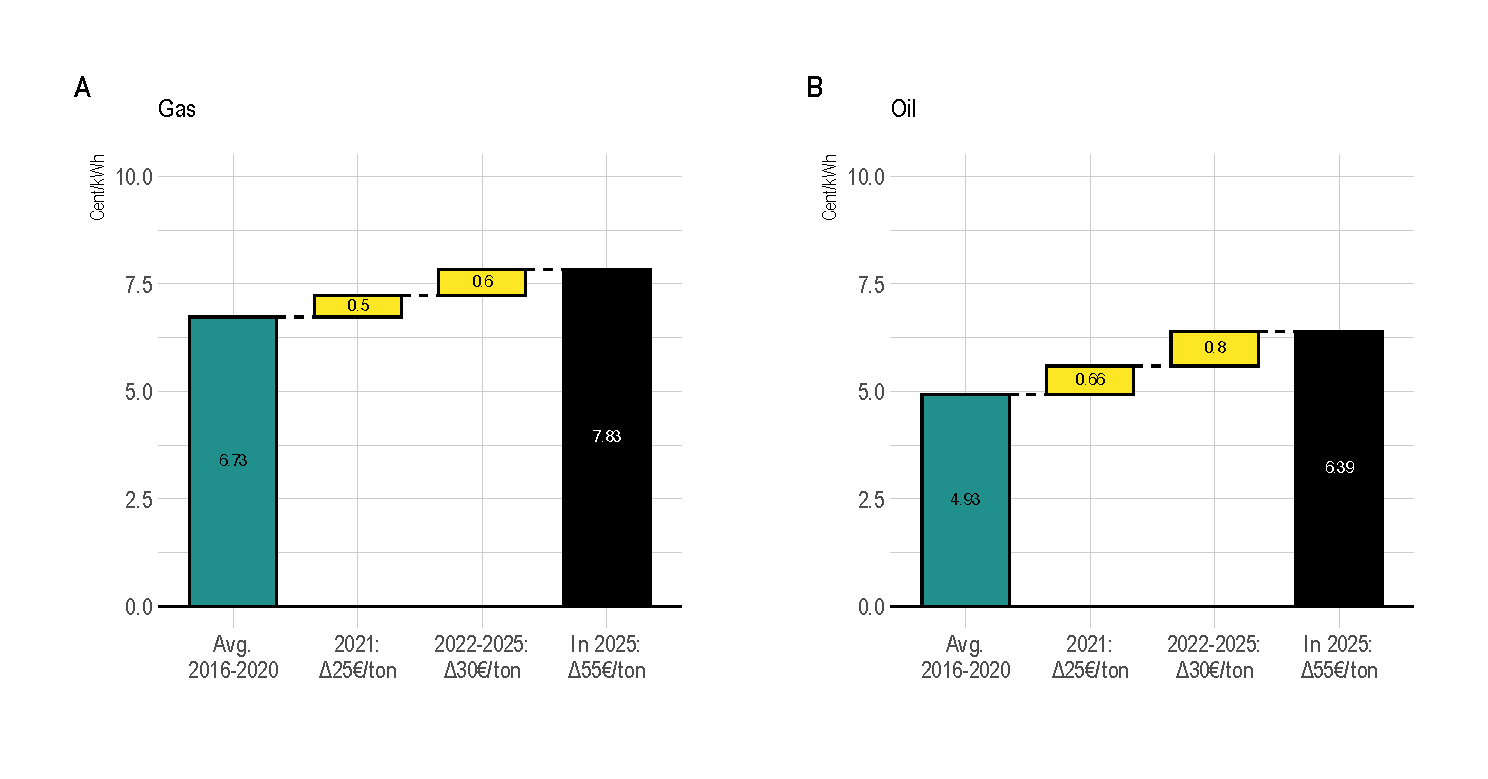
\includegraphics[width=1\linewidth]{figure/price_effect_behg} 

}

\caption[BEHG carbon price effects on gas and oil until 2025]{BEHG carbon price effects on gas and oil until 2025}\label{fig:behg}
\end{figure}
These price figures clearly indicate that relevant steering effects induced by the BEHG are likely to occur already in the next years. Higher price levels driven by the structural price component of carbon pricing can be expected to have two impact channels. The first impact channel are short-term price reactions. Consumers adjust their consumption levels for heating fuels due to higher or lower prices (\protect\hyperlink{ref-alberini_etal11}{Alberini, Gans, \& Velez-Lopez, 2011}). Short-term demand responses are therefore of direct relevance to forecasting building sector energy demand and emission levels in the coming years. The expected effect size of these short-term reactions are reflected by short-term price elasticities of heating demand which will be estimated based on empirical data in this thesis.

The second impact channel, on the other hand, is that higher prices for fossil fuels can be expected to induce long-term steering effects for investments in low-carbon heating technologies and energy efficiency. In the literature, long-term investment decisions driven by mitigation costs potentials are modeled using integrated assessment models (IAMs) for the buildings sector (e.g., \protect\hyperlink{ref-burger_etal19}{Bürger, Hesse, Köhler, Palzer, \& Engelmann, 2019}; \protect\hyperlink{ref-levesque_etal21}{Levesque et al., 2021}). Depending on the model structure, these IAM sector modules are often informed by assumptions on the price elasticities of heating demand as one of their input factor besides other parameters such as the cost of capital or substitution elasticities.\footnote{For a more detailed example of how own price elasticities of demand are taken into account in IAMs, see the model structure description of the ETSAP TIAM model in \protect\hyperlink{ref-loulou_labriet08}{Loulou \& Labriet} (\protect\hyperlink{ref-loulou_labriet08}{2008}). Since IAMs vary in their specific structure and relations other models may consider price elasticities differently.} Therefore, empirical estimates of price elasticities are also important for further analyses in the literature on the second long-term impact channel.

Additionally, the empirical assessment of the demand effect may be particularly important in the current phase of strong energy price increases following from the economic imbalances after the external shock of the COVID-19 pandemic and Russia's war of aggression on Ukraine. While the current price spikes can lead to stronger short-term demand responses, only a fraction of the response is due to the structural component of CO\textsubscript{2} pricing and -- if the effect does not last long enough to trigger significant long-term investments -- would disappear when oil and gas prices might return to lower levels. In order not to overestimate the effect of the structural pricing component of the CO\textsubscript{2} price, empirical estimates from past price reactions could be used to separate the effect into a CO\textsubscript{2} and a commodity price-related element.

\hypertarget{different-data-sources-to-estimate-price-elasticities}{%
\subsubsection*{Different data sources to estimate price elasticities}\label{different-data-sources-to-estimate-price-elasticities}}
\addcontentsline{toc}{subsubsection}{Different data sources to estimate price elasticities}

A second line of argument for the relevance of this study is that the existing empirical evidence on the price elasticity of heating demand is based on different types of data sources, but few studies have been conducted on actual billing data.

Studies on the price elasticities of heating demand rely on different types of data sources. For the case of Germany, ex-post statistical analyses for the residential buildings sector use data from social panel surveys (e.g., \protect\hyperlink{ref-rehdanz07}{Rehdanz, 2007}; \protect\hyperlink{ref-schmitz_madlener20}{Schmitz \& Madlener, 2020}; \protect\hyperlink{ref-schulte_heindl17}{Schulte \& Heindl, 2017}). In these studies, household expenditure on heating reported in the survey is usually examined as the relevant variable, but the actual level of energy consumption and energy prices are not observed. This means that, for instance, different energy contract conditions between households may obscure real consumption levels and thus affect the validity of the estimated results. The data available for this thesis is different since the energy bills do provides actual consumption and price data. Other studies using data from energy bills have previously been conducted in the United States (US) (e.g., \protect\hyperlink{ref-auffhammer_rubin18}{Auffhammer \& Rubin, 2018}).

In this context it should be noted that the data sample used in this thesis also has its weaknesses. The data does not observe demand responses at the level of individual households but at the level of multi-household buildings. Yet despite this aggregation of multiple households on the building level, I believe the informative value of estimates to be complementary to estimates from other types of data sources such as social surveys.

\hypertarget{objective}{%
\section{Research questions and objective}\label{objective}}

Against the background of the tightened emissions reduction targets, the recently introduced carbon pricing, and the sharp price increases for heating fuels, the question of the price elasticity of heating demand is once again moving to the center of public attention. The aim of this work is to investigate the price elasticity of heating demand in multi-family houses in Germany based on a large-scale sample of energy bills. The guiding research questions for the analysis are:
\begin{itemize}
\tightlist
\item
  How does a change in energy price affect the level of demand for space heating?
\item
  What other variables might affect demand for space heating and need to be taken into account so that their effects are not falsely attributed to energy prices?
\item
  And, are there potential factors for heterogeneity in the sample that may be obscured when only estimating an overall price elasticity of demand?
\end{itemize}
By using energy bills as a data source, the study aims to complement existing studies based on different sources. Furthermore, the period studied is more recent and can therefore complement older studies. Also, the analysis aims not only to estimate an overall elasticity, but also to investigate potential factors for heterogeneity. The statistical analysis aims to use several different modelling approaches, both Frequentist and Bayesian. As far as the author is aware, the Bayesian approach has not been used in previous research in this field. Furthermore, the elasticity estimates from this work may also be relevant for other countries and regions that have comparable conditions to Germany in terms of building stock and energy demand and also face the challenge of decarbonising the building sector in the coming decades. Here, my results would serve as an empirical guide to the short-term demand effects for any kind of price-related policy instrument.

The thesis is structured in six Chapters. While the first Chapter was used to provide an introduction, Chapter \ref{literature} gives an overview on the existing literature on price elasticities of space heating demand. In the following Chapter \ref{methods} the data and methods used for the analysis are laid out. Chapter \ref{results} provides the results of the analysis, which are then discussed in Chapter \ref{discussion}. Chapter \ref{conclusion} provides concluding remarks.

\hypertarget{literature}{%
\chapter{Theory and Literature}\label{literature}}

The objective of this chapter is to provide a short theoretical background on price elasticities as well as an overview of the previous research on price elasticities of heating demand. The text is organized as follows. The first part of the chapter focuses on the theoretical background and also provides a placement of the effects of varying elasticities in connection to heating demand. The second part of the chapter then moves to summarizing the empirical evidence from the literature.

\hypertarget{theory}{%
\section{Price elasticity of demand}\label{theory}}

Elasticities are one of the key concepts in mirco-economic theory. They are used to express the sensibility of one variable to a change in another. The own price elasticity of demand is one type of elasticity. It represents the magnitude of a change in consumption of a good following from a change in its own price (\protect\hyperlink{ref-pindyck_rubinfeld18}{Pindyck \& Rubinfeld, 2018}). Formally, the own price elasticity of demand \(\epsilon\) can be expressed as
\begin{equation}
\epsilon = \frac{\frac{\Delta Q}{Q}}{\frac{\Delta P}{P}} = \frac{P \Delta Q}{Q \Delta P}
\label{eq:ep}
\end{equation}
where \(\Delta P/P\) represents the percentage change in the price \(P\) of a good and \(\Delta Q/Q\) the corresponding percentage change in the quantity \(Q\) demanded of the same good. Due to budget constraints, consumers tend to consume less of a good when its price increases, which implies that under normal conditions the price elasticity of demand is negative. But the responsiveness of the demand reaction may vary across different goods. A common assumption in the econometric literature is that elasticities are constant (\protect\hyperlink{ref-varian10}{Varian, 2010}). Leading to a demand function that can be expressed by
\begin{equation}
Q = AP^{\varepsilon}
\label{eq:demand}
\end{equation}
where \(A\) represents an arbitrary constant and \(\epsilon\) again is the price elasticity of demand. Taking the logarithms of the demand function removes \(\epsilon\) from the exponent and yields
\begin{equation}
ln(Q) = ln(A) + \epsilon \; ln(P)
\label{eq:demand2}
\end{equation}
which can be referred to as the elasticity case and will reappear at a later point, when constructing the regression models to estimate price elasticities from the sample data.

To make the assumption of constant elasticity more intuitive, it seems useful to return to the subject of interest and show the behavior of demand curves for space heating under varying price elasticities of demand. Generally, the literature distinguishes between three different types of elasticities. If the demand response for a good is greater than the change in its price (\(\epsilon < -1\)), it is called price elastic. If the demand response is exactly equal to the change in price (\(\epsilon = -1\)), it is said to be unit-elastic. Finally, if the demand response is smaller than the price change (\(0 > \epsilon > -1\)) -- and therefore indicating a lower responsiveness -- it is called price inelastic (\protect\hyperlink{ref-pindyck_rubinfeld18}{Pindyck \& Rubinfeld, 2018}).\footnote{It should be noted that in the literature the minus of the demand elasticity \(\epsilon\) is sometimes omitted, as it is assumed that it is generally negative. However, I personally find it more intuitive not to do so -- especially when working empirically where positive estimates are a possibility -- and will therefore continue to use the negative values in this thesis.}

Figure \ref{fig:elasticities-conceptual} visually represents these different price elasticities for the demand of space heating.\footnote{Please note that in the graph, energy price as the independent variable is plotted on the horizontal axis and energy demand as the response variable on the vertical axis. I consider this convention -- which is common in most of science -- to be more intuitive than the traditional Marshallian cross diagram in Economics, where the price is plotted on the vertical axis.} To construct the demand curves, a common arbitrary intersection point is chosen for the curves. Specifically, this intersection has a demand value of 130 kilowatt hours (kWh) per square metre (sqm) and a price of 6 cents per kWh. These values can be considered realistic for an average building in Germany, as we will see later in this thesis when working with the sample data.
\begin{figure}

{\centering 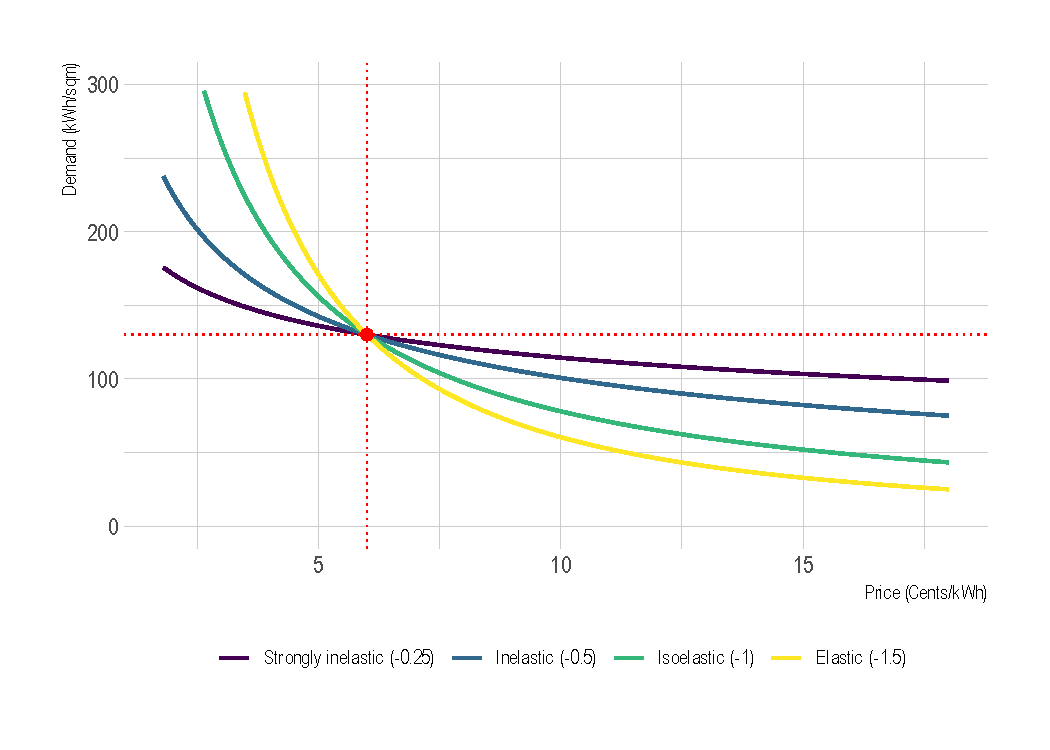
\includegraphics[width=1\linewidth]{figure/elasticities_plot} 

}

\caption{Demand curves with different price elasticities of demand}\label{fig:elasticities-conceptual}
\end{figure}
The graph shows a total of four demand curves. In addition to the unit-elastic curve (\(\epsilon = -1\)), there is also an elastic (\(\epsilon = -1.5\)) and two inelastic (\(\epsilon = -0.25, \epsilon = -0.5\)) demand curves. The special feature of the unit elastic demand curve is that it gives the same result for total expenditure on heating costs for all combinations of price times demand. This is not the case with the other elasticities. First, a look to the right of the intersection (higher prices). In the elastic case (yellow curve), total expenditures fall when the price is higher, which means that households can adjust their demand downwards more. In the opposite, inelastic cases (purple and blue curves), on the other hand, households would reduce their demand less and therefore also have higher total expenditure. Conversely, to the left of the intersection point (lower prices), more elastic demand (yellow curve) leads to a higher level of energy demand and thus also to higher total expenditure than in the inelastic cases (purple and blue curves), where demand changes only gradually.

If we now take a step back and consider what kind of good the demand for space heating represents and what price elasticity of demand one might expect, it seems reasonable to assume that the elasticity is rather inelastic. There are two indications leading to this assumption. First, heating energy is to be regarded as an essential good that is associated with a minimal level of demand -- especially in the winter months. Essential goods tend to follow a more inelastic demand pattern than other types of goods (\protect\hyperlink{ref-gwartney76}{Gwartney, 1976}). Households can only reduce their demand to a certain extent (right side of the intersection), but on the other hand, they do not have a strong rationality for a large increase in heating demand beyond a comfortable level of warmth (left side of the intersection). The second indication for a rather inelastic demand is that due to the dependency on the existing heating system -- especially for the tenant households investigated in this thesis -- there is not really a viable option to substitute space heating from one source with space heating from another.

Another important dimension for distinguishing different price elasticities of demand is time. More precisely, the time that elapses between a price signal and the measurement of the demand response. Here, the literature distinguishes between short-term and long-term price elasticities (also called short- and long-run elasticities) (\protect\hyperlink{ref-pindyck_rubinfeld18}{Pindyck \& Rubinfeld, 2018}). Short-term elasticities are those that are estimated in temporal proximity to the price change -- in this case, that would be the energy price change within a billing year and the associated change in demand in the same period (or in the year after the price change). Long-term elasticities, on the other hand, imply that more time has elapsed for consumers to fully adjust to a price change and also to make long-term investment decisions that would change the overall level of demand (\protect\hyperlink{ref-pindyck_rubinfeld18}{Pindyck \& Rubinfeld, 2018}). For the subject at hand, such decisions may include changes in the isolation of a building or an exchange of the heating system. Thus, long-term demand elasticities tend to be larger than their short-term counterparts (\protect\hyperlink{ref-schmitz_madlener20}{Schmitz \& Madlener, 2020}). Therefore, the two types can be seen as mirroring the two different channels through which a pricing policy can influence consumer behavior (see Section \ref{relevance}).

In the literature, long-term price elasticities are usually estimated using dynamic models, where the elasticity estimated between two periods represents a fraction of the long-term elasticity (e.g., \protect\hyperlink{ref-alberini_etal11}{Alberini et al., 2011}). However, I have chosen follow the example of \protect\hyperlink{ref-schmitz_madlener20}{Schmitz \& Madlener} (\protect\hyperlink{ref-schmitz_madlener20}{2020}) and only estimate short-term elasticities.This is because I believe that the long-term approaches do not apply well to the given context in which I am analyzing a subset of the total residential building segment consisting of rental buildings where households have relatively few opportunities to make long-term adjustments that would significantly affect the energy efficiency or carbon intensity of the energy of their apartments.

\hypertarget{review}{%
\section{Literature review}\label{review}}

The study of the price elasticity of energy demand is a broad field of academic research which also has a long history dating back to the mid-twentieth century (e.g. \protect\hyperlink{ref-cutler41}{Cutler, 1941}; \protect\hyperlink{ref-houthakker51}{Houthakker, 1951}). In the more recent past, as well a large nnumber of academic studies have been published. These studies differ considerably in terms of their focus and design. Several conceptual factors can systematically influence the elasticity estimates. The most important of these factors is the type of energy application analysed: The price responsiveness of household space heating demand has only limited informative value for the price responsiveness of electricity demand or transport fuel demand. The same is true for varying consumer groups: Households are likely to react differently to energy price changes than industrial consumers. Beyond, other conceptual factors which may as well affect estimates are the statistical methods used (time-series analysis, panel analysis, cross-sectional analysis), varying sources of data (national accounts, aggregate sector-level data, micro-data), varying spatial and temporal focus, measurement heterogeneity, and price trends (\protect\hyperlink{ref-csereklyei20}{Csereklyei, 2020}; \protect\hyperlink{ref-miller_alberini16}{Miller \& Alberini, 2016}). While many of the earlier studies either had only a national granularity or, when using micro data, focused predominantly on the US or European countries, a considerable number of studies have also been published recently that cover emerging countries (especially China) as well as other countries.

\textbf{Meta-estimates as first indication of elasticity magnitudes}

To organize this comprehensive body of literature with a wide range of energy applications, meta-studies do serve as a good starting point. The recently published meta-analysis by \protect\hyperlink{ref-labandeira_etal17}{Labandeira, Labeaga, \& López-Otero} (\protect\hyperlink{ref-labandeira_etal17}{2017}) is particularly suitable for this purpose, as it covers a broad spectrum of energy uses and thus goes beyond previous meta-analyses that primarily focus on the elasticity of petrol demand. I will therefore first delve into the aforementioned meta-analysis before turning to a subset of selected studies that take a closer look at the specific issue of price elasticities for space heating demand in the residential buildings sector.

In their analysis, \protect\hyperlink{ref-labandeira_etal17}{Labandeira et al.} (\protect\hyperlink{ref-labandeira_etal17}{2017}) include a total of 428 papers, all published between 1990 and 2016. For the demand of natural gas, they find an average short-term (long-term) price elasticity of -0.18 (-0.57) based on 230 individual estimates. And for heating oil they find a comparable average short-term (long-term) elasticity of -0.19 (-0.54), which, however, is based on only 44 individual estimates (\protect\hyperlink{ref-labandeira_etal17}{Labandeira et al., 2017}). An average elasticity for space heating -- which is generally less focused on in the literature due to its relatively low prevalence -- is not given.

The above average estimates of the price elasticity of demand for gas and oil, however, come with an important caveat. While they are broken down by energy carrier, they are drawn from a wide range of consumer groups. This means that the underlying studies include not only those that examine demand response patterns for residential consumption, but also others that examine these patterns for the commercial building stock and/or the industrial sector. \protect\hyperlink{ref-labandeira_etal17}{Labandeira et al.} (\protect\hyperlink{ref-labandeira_etal17}{2017}) also provide average price elasticities stratified by consumer groups, but these are on the other hand not clustered by energy source. When differentiated along the dimension of consumer groups, they report that the average estimates are slightly higher in the residential household sector (short-term: -0.22; long-term: -0.62) than in the industrial sector (short-term: -0.17; long-term: -0.51), which seems reasonable given that households likely have more ability to change their level of demand than the industrial sector with more fixed production patterns and the ability to forward costs. Overall, however, the average elasticity estimates are all in a similar size range and together convey the message that demand is strongly inelastic in the short-term, confirming the theoretical arguments that energy is an essential good in many applications and also has limited substitutability (see section \ref{theory}).

The meta-estimates are useful in providing a high-level overview. However, as already mentioned, they include estimates from a wide range of energy applications that not necessarily reflect the demand response for the specific application of space heating in residential buildings. Furthermore, they are average estimates which may have the effect of masking discrepancies and variations between studies. Therefore, the following section presents individual studies that explicitly focus on the space heating demand of the residential sector.

\textbf{Selected studies on space heating in the residential buildings sector}

The space heating demand of the residential sector represents a subset of the full literature stream. The selected studies were chosen based on the criteria that they correspond to the focus of this work and are of good quality (peer-reviewed journal articles). A summary of the studies is provided in Table \ref{tab:estimates-literature}.

There are three earlier studies that have a spatial focus on Germany. The first study was conducted by \protect\hyperlink{ref-rehdanz07}{Rehdanz} (\protect\hyperlink{ref-rehdanz07}{2007}), who estimates price elasticities for different energy carriers for residential heating demand. She uses social survey data on household-level heating expenditures from the Socio-Economic Panel (SOEP) in the years 1998 and 2003. Methodologically, a cross-sectional statistical analysis with dummy variables is conducted for the two years -- in other words, no panel structure is used. In contrast to the average meta-estimates presented in the previous section, the study finds that demand for heating oil has a high elasticity of -1.68 to -2.03, depending on the model specification. For gas, the results indicate a less elastic demand between -0.44 and -0.63, also depending on the model used. Therefore the study concludes that the type of fuels can have a strong influence on the price sensitivity of households (\protect\hyperlink{ref-rehdanz07}{Rehdanz, 2007}).
\begin{table}[]
\centering
\caption{Selected studies on the price elasticity of heating demand}
\label{tab:estimates-literature}
\resizebox{\textwidth}{!}{%
\begin{tabular}{@{}llll@{}}
\toprule
\textbf{Study} & \textbf{Type of data used} & \textbf{\begin{tabular}[c]{@{}l@{}}Energy \\ carrier\end{tabular}} & \textbf{\begin{tabular}[c]{@{}l@{}}Short-term\\ price elasticities\end{tabular}} \\ \midrule
 &  &  &  \\
{\ul \textit{Studies within Germany}} &  &  &  \\
\multirow{2}{*}{Rehdanz (2007)} & \multirow{2}{*}{\begin{tabular}[c]{@{}l@{}}Social survey, panel data (SOEP),\\ all types of buildings, 1998 and 2003\end{tabular}} & Gas & -0.44 to -0.63 \\
 &  & Oil & -1.68 to -2.03 \\
Schmitz and Madlener (2020) & \begin{tabular}[c]{@{}l@{}}Social survey, panel data (SOEP), \\ all types of buildings, 1996-2014\end{tabular} & (All) & -0.31 to -0.43 \\
Schulte and Heindl (2017) & \begin{tabular}[c]{@{}l@{}}Social survey, panel data (EVS),\\ all types of buildings, 1993-2008\end{tabular} & (All) & -0.50 \\
 &  &  &  \\
{\ul \textit{Studies outside of Germany}} &  &  &  \\
Alberini et al. (2011) & \begin{tabular}[c]{@{}l@{}}US, household-level social survey, \\ 50 metropolitan areas, panel data, 1995-2007,\\ only single-family homes and duplexes\end{tabular} & Gas & -0.57 to −0.69 \\
Auffhammer and Rubin (2018) & \begin{tabular}[c]{@{}l@{}}US, energy billing data, household-level, \\ only California, panel data, 2003-2014\end{tabular} & Gas & -0.17 to -0.23 \\
\begin{tabular}[c]{@{}l@{}}Leth-Petersen and \\ Togeby (2001)\end{tabular} & \begin{tabular}[c]{@{}l@{}}Denmark, apartment-block level (\textgreater{}1,500 sqm),\\ panel data, 1984-1995\end{tabular} & Oil & -0.08 \\
 &  & District heating & -0.02 \\
\multirow{2}{*}{Meier and Rehdanz (2010)} & \multirow{2}{*}{\begin{tabular}[c]{@{}l@{}}UK, household-level social survey,\\ panel data 1991-2005\end{tabular}} & Gas & -0.34 to -0.56 \\
 &  & Oil & -0.40 to -0.49 \\
Metcalf and Hassett (1999) & \begin{tabular}[c]{@{}l@{}}US, household-level, panel data, \\ 1984, 1987 and 1990\end{tabular} & Gas & -0.48 to -0.71 \\ \bottomrule
\end{tabular}%
}
\end{table}
In a more recent study, also based on the SOEP social survey data but covering a more comprehensive time period between 1996 and 2014, \protect\hyperlink{ref-schmitz_madlener20}{Schmitz \& Madlener} (\protect\hyperlink{ref-schmitz_madlener20}{2020}) find a price elasticity of heating and hot water demand of -0.31 to -0.43, depending on model specifications. They do not differentiate the elasticities by energy carrier. The price elasticities are derived from household expenditure elasticities, as demand is not directly observed. In contrast to \protect\hyperlink{ref-rehdanz07}{Rehdanz} (\protect\hyperlink{ref-rehdanz07}{2007}), the study uses a panel structure where observations are clustered by household and year using fixed effects. This produces much lower price elasticity estimates, which are more consistent with the meta-estimates presented in the previous section. Moreover, the study discovers that price elasticity is heterogeneous across different socio-economic groups. Given the household-level information at their disposal, they find that higher-income households are less sensitive to energy price changes than lower-income households. Likewise, homeowners show less sensitivity than renters (\protect\hyperlink{ref-schmitz_madlener20}{Schmitz \& Madlener, 2020}).

Also for Germany, \protect\hyperlink{ref-schulte_heindl17}{Schulte \& Heindl} (\protect\hyperlink{ref-schulte_heindl17}{2017}) investigate the price and expenditure elasticities of private energy demand in Germany between 1993 and 2008. For their analysis, they use survey data from the \emph{Einkommens- und Verbrauchsstichprobe (EVS)} and analyse them with a demand system approach (in particular, they estimate a quadratic expenditure system). For space heating, they find an own-price elasticity of -0.50 across all households. They further observe that the price elasticity changes with the level of total household expenditure, with households in higher expenditure strata reacting more strongly to price changes (\protect\hyperlink{ref-schulte_heindl17}{Schulte \& Heindl, 2017}). Put differently, this means that following an increase in price level low income households tend to lower energy demand to a lesser extent as compared to households with a higher income. Thus, in relation to the income dimension the results must be understood as contradictory to those of \protect\hyperlink{ref-schmitz_madlener20}{Schmitz \& Madlener} (\protect\hyperlink{ref-schmitz_madlener20}{2020}).

All three studies on Germany rely on data from household-level social surveys. Therefore, the studies take a strong perspective on the impact of household income on energy price sensitivity. As the data for this study is aggregated at the building-level and not at the household-level, however, the focus of this thesis is to some extent different. The focus is rather on the overall price response based on actual price and consumption values, which are not available in the social surveys, and on the response in interaction with other characteristics and changes at the building level.

Besides the studies focusing on Germany, Table \ref{tab:estimates-literature} also reports the evidence from five selected international studies focusing on the price elasticities of space heating demand. \protect\hyperlink{ref-alberini_etal11}{Alberini et al.} (\protect\hyperlink{ref-alberini_etal11}{2011}) examine household demand for gas (and electricity) in single-family homes and duplexes using household-level social survey data in 50 metropolitan areas in the United States (US) over the period 1995-2007. As a modelling approach, they use static and dynamic panel models. For the static models reflecting the approach taken in this thesis, they find an own price elasticity of private gas demand between -0.57 and -0.69, depending on the model specification. These estimates are in their magnitude comparable to the results of an earlier study by \protect\hyperlink{ref-metcalf_hassett99}{Metcalf \& Hassett} (\protect\hyperlink{ref-metcalf_hassett99}{1999}) who use the 1984, 1987 and 1990 waves of the US Residential Energy Consumption Survey (RECS) to examine homeowners' investments in energy efficiency measures and as part of their study find price elasticities of residential gas demand to range between −0.48 and −0.71. In contrast to these estimates, a recent study by \protect\hyperlink{ref-auffhammer_rubin18}{Auffhammer \& Rubin} (\protect\hyperlink{ref-auffhammer_rubin18}{2018}) finds that the short-term price elasticity of residential gas demand is even more inelastic, ranging from -0.17 to -0.23, not for the whole US but for California in particular. The study by \protect\hyperlink{ref-auffhammer_rubin18}{Auffhammer \& Rubin} (\protect\hyperlink{ref-auffhammer_rubin18}{2018}) is especially interesting for this thesis because it is the only one that also uses energy billing data. The data analysed covers the period 2003-2014 and consists of monthly energy bills at the household-level. So although the type of data source used to derive the estimates is the most similar to the approach taken in this thesis, there are still two relevant differences: firstly, gas tariffs in the US nay change monthly rather than annually, as is the case in the German dataset used for this analysis, and secondly, the data in \protect\hyperlink{ref-auffhammer_rubin18}{Auffhammer \& Rubin} (\protect\hyperlink{ref-auffhammer_rubin18}{2018}) relates to individual households rather than the aggregate building-level.

In addition to these three studies focusing on the US, Table \ref{tab:estimates-literature} also contains the results of a Danish study by \protect\hyperlink{ref-leth-petersen_togeby01}{Leth-Petersen \& Togeby} (\protect\hyperlink{ref-leth-petersen_togeby01}{2001}). They use a panel data approach and analyse data from the period 1984-1995. Interestingly, they also use the building-level as the level of analysis. More specifically, they study apartment buildings with a base area of more than 1,500 square meters (sqm) in Denmark. As an empirical strategy, they rely on fixed effects models. As a result, they find very inelastic demand responses for space heating. For oil, the short-term price elasticity is found to be -0.08 and for district heating as low as -0.02, meaning almost no demand response to a changing price at all. Another study by \protect\hyperlink{ref-meier_rehdanz10}{Meier \& Rehdanz} (\protect\hyperlink{ref-meier_rehdanz10}{2010}) looks at the United Kingdom (UK) and analyses a household-level social survey panel for the 15-year period 1991-2005. For their model they use a log-linear approach. They find that the short-term price elasticity of demand for gas ranges from -0.34 to -0.56, depending on the specification. For residential oil demand, the results are in the same order of magnitude, but narrower, between -0.40 and -0.49. In addition, they find that the type of occupant is a relevant dimension for a different price responsiveness. While renters adjusted their demand level more, homeowners showed a more inelastic response.

\textbf{Synthesis of estimates from the literature}

When summarizing the literature on the price elasticity of residential space heating demand presented previously, commonalities and differences emerge. The most important commonality is that the price elasticity of energy demand in general and household space heating demand in particular is inelastic in almost all empirical estimations. But at the level of individual studies, differences in the magnitude of the estimates persist. While the meta-results by \protect\hyperlink{ref-labandeira_etal17}{Labandeira et al.} (\protect\hyperlink{ref-labandeira_etal17}{2017}) as well as a number of individual studies indicate a strongly inelastic demand response (e.g. \protect\hyperlink{ref-auffhammer_rubin18}{Auffhammer \& Rubin, 2018}; \protect\hyperlink{ref-leth-petersen_togeby01}{Leth-Petersen \& Togeby, 2001}), other individual studies still indicate an inelastic but stronger demand response (e.g., \protect\hyperlink{ref-alberini_etal11}{Alberini et al., 2011}; \protect\hyperlink{ref-meier_rehdanz10}{Meier \& Rehdanz, 2010}; \protect\hyperlink{ref-metcalf_hassett99}{Metcalf \& Hassett, 1999}; \protect\hyperlink{ref-rehdanz07}{Rehdanz, 2007}; \protect\hyperlink{ref-schmitz_madlener20}{Schmitz \& Madlener, 2020}; \protect\hyperlink{ref-schulte_heindl17}{Schulte \& Heindl, 2017}). These differences in magnitude may be partly due to the different local and temporal conditions of the studies or due to differences in the data and methodology. Such aspects may also include behavioral aspects related to a specific population. Figure \ref{fig:literature-estimates-plot} graphically represents the short-term elasticity estimates from Table \ref{tab:estimates-literature}. As a synthesis, all studies that focused on Germany found somewhat more sensitive price elasticities ranging from -0.3 to -0.6.\footnote{Note that the extreme results of \protect\hyperlink{ref-rehdanz07}{Rehdanz} (\protect\hyperlink{ref-rehdanz07}{2007}) for the carrier oil, which come only from a cross-sectional regression analysis, are omitted here. Since only two isolated periods are considered, these results must be considered more prone to extreme results than is the case with a longer panel.} And also most estimates from other countries can be allocated to that range of price sensitivity.
\begin{figure}

{\centering 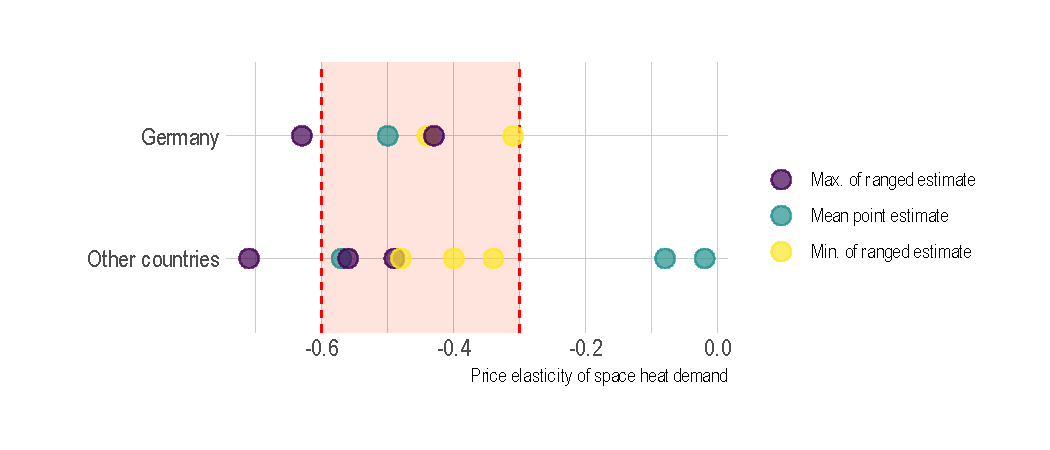
\includegraphics[width=1\linewidth]{figure/plot_literature_estimates} 

}

\caption{Price elasticity of space heat demand estimates from individual studies}\label{fig:literature-estimates-plot}
\end{figure}
Importantly, another common feature that links all the individual studies presented is that they do not focus on one-off extreme price shocks as an identification strategy, but on gradual price developments. They are mostly built around a panel data set covering a longer period of time. The period examined in this study also covers more than a decade with rather gradual price developments. This should therefore be considered an important condition that facilitates the comparability of the results of this study with the estimates presented in the literature.

\hypertarget{conceptual-model}{%
\section{Conceptual model development}\label{conceptual-model}}

In the previous two subsections, the theoretical background on price elasticities of demand (see section \ref{theory}) and previous evidence from the literature on household responsiveness to energy price changes (see section \ref{review}) have been presented. To synthesize this basis, this subsection uses both theory and approaches from previous studies to develop a conceptual model. The aim is to identify relevant determinants for the level of space heating demand of private households and to justify their relevance. The conceptual model will then be transferred into a statistical model and empirically examined in the further course of this work.

\textbf{Price elasticity}

The starting point is the relationship between energy price and space heating demand, the assumption from the theory of price and demand being that the demand for space heating is influenced by the changes in the energy price. If the energy price goes up, energy demand moves down along the demand curve and vice versa (see Figure \ref{fig:elasticities-conceptual}). Expressed in a statistical terminology, this implies that space heat demand is the response variable of a model and energy price the main explanatory variable.

To support the development of the conceptual model visually, Figure \ref{fig:dag} depicts it as a directed acyclic graph (DAG). At the center, space heat demand is shown, the variance of which is to be explained (yellow bubble). The effect of energy price (purple bubble) on space heating demand represents the \emph{price elasticity} and is therefore highlighted by the red arrow.
\begin{figure}

{\centering 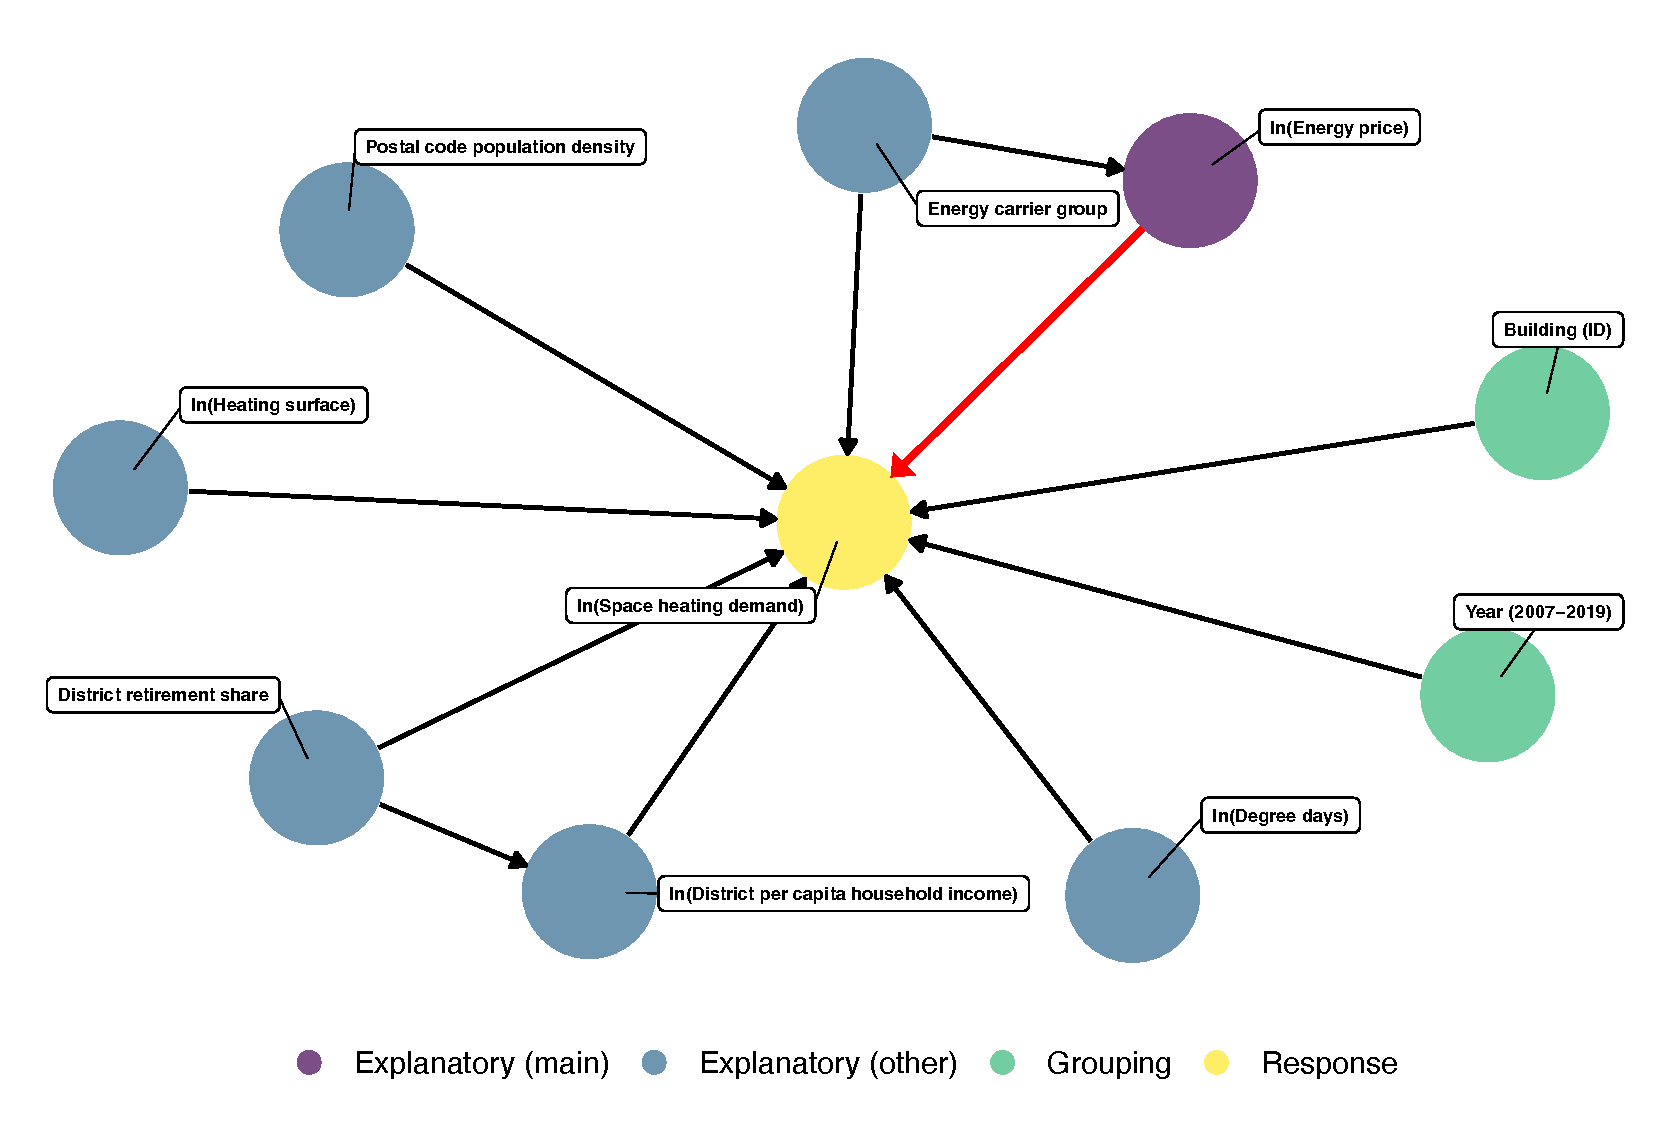
\includegraphics[width=1\linewidth]{figure/dag_red} 

}

\caption[Conceptual model as directed acyclic graph]{Conceptual model as directed acyclic graph}\label{fig:dag}
\end{figure}
In addition to energy price, there are an array of other variables that may influence the level of space heating demand. These are shown in the DAG as additional explanatory variables (blue bubbles) and as grouping variables (green bubbles). To determine the set of additional relevant variables, a structured approach was used. First, the recent work of \protect\hyperlink{ref-schmitz_madlener20}{Schmitz \& Madlener} (\protect\hyperlink{ref-schmitz_madlener20}{2020}) was considered as a suitable starting point to create a list of variables. Second, the other studies presented in Section \ref{review} were then used to cross-validate the initial list of variables as well as to screen for further ones. This structured approach led to the variables being justified in terms of their potential effect on space heating demand in the following.

\textbf{Climatic condition}

Firstly, the consideration of the local climatic condition in a billing period is of importance, as it can have a strong effects on the space heating demand (\protect\hyperlink{ref-hesse20}{Heße, 2020}). Due to their high relevance, all studies presented in Section \ref{review} consider and control for climatic conditions. Usually, climatic conditions are approximated by the outdoor temperature over a defined period of time and aggregated to periodical (heating) degree days. The basic intuition for the influence of varying climatic conditions is that with lower mean outdoor temperatures, transmission heat losses increase and thus the demand for space heating increases to compensate for indoor heat losses. In line with \protect\hyperlink{ref-vdi13}{VDI} (\protect\hyperlink{ref-vdi13}{2013}), degree days in this study are defined as the temperature difference between a mean room temperature of 20°C and the daily mean of the outdoor temperature, provided it is below the heating limit of 15°C.\footnote{It should be noted that the definition of degree days used here differs from the internationally frequently used definition of heating degree days (HDD), which is calculated by difference between the average outdoor temperature below a heating threshold over time -- regardless of an additionally defined room temperature. In this thesis, the VDI based definition of \emph{degree days} was chosen, as this is the common methodology in Germany. It is, for example, also used to create a comparable scoring for building energy performance certificates (see \protect\hyperlink{ref-halbig_namyslo14}{Halbig \& Namyslo} (\protect\hyperlink{ref-halbig_namyslo14}{2014})).} Lower mean outdoor temperatures are associated with a higher aggregated number of degree days in a period. Consequently, one would expect a higher space heating demand when the degree days in an annual heating cycle are higher and vice versa. Varying degree days may occur on a temporal (one year is warmer/cooler than another) but also on a spatial scale (places at higher altitudes or in the interior of the continent have structurally lower temperatures).

\textbf{Building-level characteristics}

In addition, two building-level characteristics are included in the model as additional explanatory variables. First, the size of a building can influence the heat demand, as in larger buildings the ratio between the external surface of the building and the heating surface decreases. Thus, the relative share of transmission heat losses per unit of heating surface is lower correspondingly. Following this rationale, it must be assumed that in buildings with a larger heating surface -- which approximates the size of a building -- the space heating demand per unit is lower if all other factors are to remain the same.\footnote{While this paper uses heating area as a continuous variable, other studies with a less detailed database often use building size categories, which can be seen as a similar approach.}

Second, the type of energy carrier used for the heating system is another building-level characteristic, which is considered in almost all previous studies (see Section \ref{review}). The intuition for the inclusion of the energy carrier as a categorical control variable (oil, gas, district heating) is that different carrier types are associated with different heating technologies, which can lead to structural differences in energy use and efficiency. This effect may be further amplified by the fact that certain energy carriers were more commonly introduced in certain periods in the past. This means that, for example, an average oil heating system may be older and thus less energy efficient than an average gas heating system due to technological progress.

\textbf{District socio-economic variables}

Besides building-related characteristics, socio-economic variables may also affect the level of heating demand. In the literature that draws its data from social surveys, household-level socio-economic information such as income, number of inhabitants, age, education level or employment status is usually part of the core survey data and therefore considered as control variables in the analysis. This study, in contrast, relies on energy billing data at the building level, which can provide a more accurate picture of actual energy demand and prices than social surveys, but in return does not provide socio-economic information, neither at the household nor at the aggregated building level. Nevertheless, previous studies make a strong case for the inclusion of socio-economic variables. Thus, to incorporate their perspective, three socio-economic variables at the district or postal code level are included in the conceptual model. The rationale being that they may capture overlaying socio-economic effects at an higher level of aggregation.

The first of the three variables is per capita household income at the district-level. In line with most of the literature, one would expect lower income to lead to lower heating demand as households have fewer funds at their disposal. However, it could also be that income at the district level is more of an approximation of the general affluence of a district and therefore effects such as lower economic resources available for investment in building efficiency outweigh a household budget effect of demand and possibly lead to the opposite outcome. Secondly, the district retirement share is considered as an additional variable. Here, the intuition is that with high retirement rates in a district more people spend more of their time at home which may lead to a rise in space heat demand. Lastly, the population density within a postal code area is considered to observe if there may be structural differences in heating demand between densely populated metropolitan areas on the one hand and sparsely populated rural areas on the other.

\hypertarget{methods}{%
\chapter{Methods}\label{methods}}

\hypertarget{data}{%
\section{Data description and pre-processing}\label{data}}

To translate the conceptual model set up in Section \ref{conceptual-model} into a statistical model that can be used to empirically investigate the price elasticity of space heating demand, data from multiple sources were combined.

\textbf{Energy billing dataset}

The key dataset is a large-scale building-level panel of energy bills made available though the Climate Policy Department at DIW Berlin. The data originates from the energy- and billing service provider ista Deutschland GmbH and was provided for scientific use.\footnote{Due to the sensitivity of the data, it is to be classified as confidential. Access was exclusively via DIW Berlin's internal servers. Due to data protection regulations, it is not possible to make the data available to external parties for the purpose of reproducing the results.} The sample contains information on an average of multi-unit residential buildings in Germany and ranges from 2007 to 2019.\footnote{On the basis of exemplary heating bills provided by ista, it was possible to determine that this was also the case for the data in the billing sample.} The smallest buildings observed have two living units; single-family houses with just one unit are not observed. The observations in the dataset represent annual heating bills at the building-level. The dataset contains the two main variables for the analysis: space heating demand and energy price. It also contains additional building-level information including the heating surface, the number of housing units, the type of energy carrier used for heating. The dataset also provides a building-level ID and the billing dates suitable to create a panel structure.

\textbf{Space heat demand (kWh/sqm/a):} The demand data in the billing dataset is provided as total energy consumed per building and per annual billing period in kilowatt hours (kWh). To isolate the share of energy consumed for the purpose of space heating, the share of energy used for hot water production is deduced for those buildings where hot water production is also done via the central heating system. In a second step, in order to obtain a comparable metric for the differently sized buildings in the sample, the total space heating demand at building level is divided by the building heating surface in square meters (sqm). This results in the annual space heat demand per square meter as the demand variable. For a summary of the variables and their data sources see Table \ref{tab:variables}.

\textbf{Energy prices (Cents/kWh):} The structure of the price data in the dataset is similar to that of the demand data. The energy price data is provided as total annual costs at the building-level in Euros. Again, relying on the supplementary information on the relative shares of energy use for space heating and hot water generation in buildings where hot water is provided via the central heating system, the cost share for space heating alone is identified. In a second step, the cost share for space heating is then translated into average per-unit costs by dividing total costs for space heating by the respective demand for space heating in kWh. To make the cost scale more intuitive, prices are furthermore converted from Euros to Cents. This yields a per-unit energy price variable (Cents/kWh). Additionally, since energy prices are provided as nominal prices, they are deflated using the German annual consumer price index (CPI) with 2015 as the index year (\protect\hyperlink{ref-destatis21}{DESTATIS, 2021b}). The use of the CPI to deflate energy prices represents the standard procedure in the literature, which is also used by \protect\hyperlink{ref-schmitz_madlener20}{Schmitz \& Madlener} (\protect\hyperlink{ref-schmitz_madlener20}{2020}), for example.

Energy contracts for private households in Germany usually consist of a fixed cost component (flat-rate basic charge) and a variable cost component (consumption-based price per kWh).\footnote{On the basis of exemplary heating bills provided by ista, it was possible to determine that this was also the case for the data in the billing sample.} The data does not contain a breakdown of fixed and variable costs, but only the total costs, which are then converted into average costs per-unit (the sum of fixed and variable costs divided by the quantity demanded) as described in the previous paragraph. There is much debate in the literature about whether the household demand response to changes in energy prices depends on the average price or instead on the marginal price. The use of marginal prices would be necessary if the variable price component were to change based on the quantity consumed (``block pricing'') and could also be dynamically adjusted by the utility, as is the case for many private household contracts in the USA, for example (see \protect\hyperlink{ref-auffhammer_rubin18}{Auffhammer \& Rubin, 2018}). Since those factors do not apply for the energy contracts underlying the billing data used in this thesis, I assume the use of the average per-unit energy price to be suitable, as it was also done in other studies (e.g., \protect\hyperlink{ref-metcalf_hassett99}{Metcalf \& Hassett, 1999}; \protect\hyperlink{ref-rehdanz07}{Rehdanz, 2007}; \protect\hyperlink{ref-schmitz_madlener20}{Schmitz \& Madlener, 2020})

Another problem is whether the demand decisions depend on the price in the same period or on the price of the previous period, so that the calculation of the previous period influences the current demand decisions. Following the approach of \protect\hyperlink{ref-schmitz_madlener20}{Schmitz \& Madlener} (\protect\hyperlink{ref-schmitz_madlener20}{2020}), I generally construct the model with the price in the same period. However, to check the robustness of the results, I also run models with the price of the previous period.

\textbf{(Billing) Year:} The billing data contains the exact dates of the billing period of an individual building. While most billing periods mirror the calendar year, some buildings have billing periods occurring during the year. Therefore, the start and end dates of the billing periods are used to make an allocation to billing years. For billing periods during the year, the allocation is based on which of the two calendar years contains the majority of days in the billing period.

\textbf{Energy carrier group:} There are three main types of energy carriers included in the dataset: Gas, oil, and district heating. To obtain these three categories, energy carrier descriptions from the dataset are grouped under these categories (e.g, \emph{Gas low} and \emph{Gas high} are grouped under \emph{Gas}). In addition, all other heating carriers which have only limited occurrence in the sample (e.g.~electricity for heat pumps, coal combustion) are grouped under the category \emph{Others} and later excluded from the analysis due to the relatively small number of observations and heterogeneity of carrier types within the group (see Section \ref{workflow}).

\textbf{Heating surface (sqm):} Information on the heating surface of a building is given in square meters at building-level. The heating surface does not correspond to the total floor area of a building, as it excludes the unheated surfaces within a buildings (e.g., building corridors or basements). Heating area was chosen over the number of housing units as an alternative approximation for the size of a building. The reasons for this are that it was assumed that the heating surface better reflects the ratio between the interior and exterior area of a building since it does not suffer from varying sizes of housing units.
\begin{table}[]
\centering
\caption{Variables and data sources}
\label{tab:variables}
\resizebox{\textwidth}{!}{%
\begin{tabular}{@{}lllll@{}}
\toprule
\textbf{Variable} & \textbf{} & \textbf{Type} & \textbf{Unit} & \textbf{Data source} \\ \midrule
 &  &  &  &  \\
\textit{\begin{tabular}[c]{@{}l@{}}Demand\\ \end{tabular}} & Space heat demand & Continuous & ln(kWh/sqm) & Ista (billing data) \\
\textit{} &  &  &  &  \\
\textit{\begin{tabular}[c]{@{}l@{}}Price\\ \end{tabular}} & Energy price & Continuous & ln(Cents/kWh) & Ista (billing data)\\
\textit{} &  &  &  &  \\
\multirow{4}{*}{\textit{\begin{tabular}[c]{@{}l@{}}Additional billing \\information\\ \end{tabular}}} & Heating surface & Continuous & ln(sqm) & Ista (billing data)\\
 & Energy carrier group & Categorical & Gas / Oil / District heating & Ista (billing data)\\
 & Building ID & Categorical & - & Ista (billing data)\\
 & Year & Categorical & - & Ista (billing data)\\
\textit{} &  &  &  &  \\
\textit{\begin{tabular}[c]{@{}l@{}}Climatic conditions\\ \end{tabular}} & Degree days & Continuous & ln(degree days) & IWU (2021) \\
\textit{} &  &  &  &  \\
\multirow{3}{*}{\textit{\begin{tabular}[c]{@{}l@{}}Socio-economic factors\\ \end{tabular}}} &  District household income & Continuous & ln(Euros/a) & Statistische Ämter (2021) \\
 & District retirement share & Continuous & \% & DESTATIS (2021a) \\
 & Postal code population density & Continuous & ln(inhabitants/sq. km) & OSM (2021), OSM (2021a) \\ \bottomrule
\end{tabular}%
}
\end{table}
\textbf{Supplementary data sources}

\textbf{Degree days:} Degree days were retrieved from an Excel tool compiled by the \emph{Institut für Wohnen und Umwelt (IWU)} at the postal code level (\protect\hyperlink{ref-iwu21}{IWU, 2021}). The degree days data from the IWU-tool builds on daily temperature data from the 800 weather stations of the German Meteorological Service (DWD) that are aggregated on a monthly basis. In the tool, the settings of a mean room temperature of 20°C and a heating limit of 15°C are chosen to reflect the VDI based definition of degree days (\protect\hyperlink{ref-vdi13}{VDI, 2013}). Furthermore, the option to assign the postal code area to the three nearest DWD weather stations with weighting according to geographical distance is chosen. This is because relying on reduce the risk of possible distortions due to differences in altitude between a single weather station and the centroid of a postal code area. The extracted monthly degree day figures per postal code area are then aggregated to annual periods on a rolling basis and matched with the annual building-level energy billing observations. The postal code level was chosen because it corresponds to the spatial information on the location of the buildings contained in the billing data and therefore represents the most accurate allocation possible.

\textbf{District per capita household income (Euros/a):} As a district-level income variable to approximate for varying incomes, the per capita disposable income of private households provided by the joint statistical portal of the federal and state governments is used (\protect\hyperlink{ref-statistischeamter21}{Statistische Ämter, 2021}). The figure includes the primary income of private households, minus transfers paid and plus transfers received. Disposable income is chosen because it can be considered the most suitable indicator for funds available for households. The district-level is chosen as it is the most granular household income statistics available.

\textbf{District retirement share (\%):} To construct the district retirement share variable, population data at the district-level with a segmentation by age groups is used (\protect\hyperlink{ref-destatis21c}{DESTATIS, 2021a}). As an approximation for the actual proportion of retirees, the percentage of persons within a district and year who are 65 years of age and older is calculated. This approach was chosen because no detailed statistics are available on the number of people in retirement at the district-level. The boundary value of 65 was chosen as the age group closest to the current retirement age in Germany and since the same threshold was also chosen in the literature (e.g., \protect\hyperlink{ref-alberini_etal11}{Alberini et al.} (\protect\hyperlink{ref-alberini_etal11}{2011}))

\textbf{(Postal code) Population density (inh./sq. km):} To generate the population density variable, data from Open Street Maps with pre-assigned population figures to postal code areas based on the 2011 Census were used (\protect\hyperlink{ref-osm21}{OSM, 2021b}, \protect\hyperlink{ref-osm21a}{2021a}). The postal code level and not the district level was chosen because, firstly, a higher granularity of data was available and, secondly, the use of districts as the level of analysis may obscure heterogeneity within districts. Especially when they are rural districts with a city. To determine the population density variable, the number of inhabitants per postal code was divided by the base area in square kilometers (sq. km), giving the population density as the average number of inhabitants per sq. km.

\hypertarget{empirical_model}{%
\section{Empirical approach}\label{empirical_model}}

\textbf{Causality with observational data}

The conceptual DAG presented in Section \ref{conceptual-model} and the derived rationales for the cause-and-effect relationships between space heat demand and energy price in an environment where the other explanatory variables also exert an effect on energy demand are all based on the assumption of causal inference. Causal inference can be described as indicating that an observed relationship between two variables is reflected by a causal link and not just mere correlation (\protect\hyperlink{ref-holland86}{Holland, 1986}). The analysis in this thesis is build on externally provided observational data. Using observational data to draw causal inference about a treatment effect -- in the given case, inference about the price sensitivity of private households for space heating demand in multi-family buildings in Germany -- is inherently difficult since the treatment is not controllable and therefore cannot be randomly assigned (\protect\hyperlink{ref-nichols07}{Nichols, 2007}). Since an experimental research design, which would arguably provide the most unbiased source of evidence, is not feasible for this research, it is all the more important to point out potential sources of bias in the estimation process relying on observational data and address those biases where possible.

\textbf{Potential sources of bias}

Reducing potential sources of bias was approached in several steps. First, the set of explanatory variables already described was used to reduce potential bias from omitted variables. This means that by taking into account, for example, degree days or the heating surface of a building, additional relevant effects on the level of heating demand are captured that might otherwise be wrongly attributed to the role of energy price alone.

On the other hand, there is also an additional gap in the data in relation to the omitted variables that cannot be fully remedied. Due to the aggregated nature of the data at the building-level, it is not possible to integrate detailed household-level socio-economic variables (e.g., household income, number of inhabitants, age, education level, or employment status) into the analysis. In other studies which build on household-level social surveys socio-economic variables have been found to be a relevant determinant of energy demand -- especially household income is a variable that has been found to exert a relevant effect (e.g., \protect\hyperlink{ref-meier_rehdanz10}{Meier \& Rehdanz, 2010}; \protect\hyperlink{ref-rehdanz07}{Rehdanz, 2007}; \protect\hyperlink{ref-schmitz_madlener20}{Schmitz \& Madlener, 2020}). To at least partially address the fact that socio-economic variables are not available at the household level, socio-economic controls at the district or postcode level are used to try to capture the underlying socio-economic effects at a higher level.

Another source of potential bias can result from data errors. In general, the use of observational data should not be considered a mechanistic process, but should be based on the application of domain-specific knowledge to critically evaluate and challenge the available data. In view of the potentially distorting effects of data errors, the use of domain-specific knowledge and expert judgement was important in cleaning and processing the energy billing dataset. The process is described in detail in the following section \ref{Workflow}. When evaluating the energy price variable, outliers are found that can be traced back to be placeholders that do not reflect the actual energy demand. If these observations had not been removed from the analysis, they would have distorted the result of the analysis.

In addition, it was checked if the measurement of the variables incorporated any systematic measurement error and concluded that a systematic error was not present. Generally, several variables used in the analysis might be subject to measurement error. For example, the degree days data are based on a spatial interpolation of the values from the three nearest DWD weather stations to the centroid of a postal code, which introduces a first layer of measurement error. It is then assumed that the degree days assigned to a postal code apply to every building within that postal code, even though there may be greater distances and differences in elevation between the centroid and the building's location representing a second layer . However, errors such as those described exemplarily for the degree days variable do not necessarily represent a problem, since a systematic deviation is required for the existence of a systematic error (bias). Rather, the described exemplary derivations from a true value for outdoor temperature indicate a random inaccuracy in the measurement of the variable, which is less serious in general and especially given the very large number of observations in the sample. The same logic applies, for example, to the construction of the energy demand variable. While aggregation at the building level introduces some inaccuracy compared to a hypothetical measurements at the household-level, it does not lead to a systematic error.

\textbf{Simultaneity problem}

Furthermore, when estimating price elasticities of demand, one additional relevant challenge for the identification of a causal effect is the potential simultaneous determination of price and demand leading to a market equilibrium
\begin{itemize}
\item
  Use of multiple estimation techniques (panel regression, Bayesian mutilevel models)
\item
  Issue of Simultaneity (See Aufhammer)
\item
  If demand is assumed to depend on the marginal block price, then price and consumption are simultaneously determined, and instrumental variable estimation techniques must be used (Burtless and Hausman, 1978; McFadden et al., 1978; Wilder and Willenborg, 1975; Hewitt and Hanemann, 1995; Reiss and White, 2005). For lack of exact information about the block rates faced by the consumers, however, we are forced to use average price.
\item
  Perhaps most importantly, research on the elasticity of demand for natural gas must also consider multiple potential sources of endogeneity. The first source of endogeneity is the classic simultaneity that stems from the fact that quantity and price result from the equilibrium in a system of equations. Unlike the electricity sector, for natural-gas customers' rates change on a monthly basis---updating as a function of gas wholesale prices paid by the retail utilities.
\item
  From Aufhammer wegen IV approach: We instrument the utilities' consumer-facing prices with the weekly average spot price of natural gas at a major natural gas distribution hub in Louisiana (the Henry Hub). This instrument is valid, as we know the formula of how utilities pass-through the price (providing a strong first stage), and the price is determined prior to within-bill consumption (strengthening the exclusion restriction).
\end{itemize}
\textbf{Frequentist estimation approach}

For the analysis, I use several statistical methods. For the full sample analysis, I rely on Frequentist estimation approaches given the large number of data points in the billing dataset. For the subsequent analysis of a stratified random subsample I rely on Bayesian methods. Generally, I follow a logic where I begin with constructing a simple model specification and then extend it to a more elaborate statistical model. The goal partly being to be able to compare model estimates by varying methods and predictors included.

To start with, I formulate the statistical model for the full sample analysis as a simple cross-sectional multiple linear regression (MLR) model based on ordinary least squares (OLS) (\protect\hyperlink{ref-bailey17}{Bailey, 2017}; \protect\hyperlink{ref-wooldridge13}{Wooldridge, 2013}):
\begin{align*}
ln(Demand) & = \alpha + \beta_1 \cdot ln(Price) + \beta_2 \cdot ln(Degree.days) + \\
 & \quad \beta_3 \cdot ln(Heating.surface) + \beta_{4} \cdot Carrier.group.oil + \\
 & \quad \beta_{5} \cdot Carrier.group.district.heating + \beta_{6} \cdot District.income + \\
 & \quad \beta_{7} \cdot District.retire + \beta_{8} \cdot Pop.density + \varepsilon 
\end{align*}
where the response variable \(ln(Demand)\) denotes the natural logarithm of the annual space heating demand per square meter, the main explanatory variable \(ln(Price)\) denotes the natural logarithm of the average energy price (Cents/kWh) in the same period. The other terms of the linear equation denote the additional explanatory variables (degree days, building characteristics, and district/postal code socio-economic variables) and \(\varepsilon\) denotes the error term of the model. Referring back to equation \eqref{eq:demand2} from the theory section, the ln-form of both sides of the equation transforms the model into the elasticity case. Therefore, the coefficient \(\beta_1\) of \(ln(Price)\) represents the price elasticity of space heating demand. For the cross-sectional OLS regression, I first run the model with \(ln(Price)\) as a sole predictor and then with the additional explanatory variables included.

In the billing dataset, there is both a building ID, which allows observations from several periods to be assigned to the same building, and information on the billing period. Thus, the data allows to go beyond cross-sectional OLS and apply panel data estimation techniques. In the OLS estimation shown above, observations from various buildings and years are treated to be systematically no different from each other. Panel data methods, on the contrary, are rooted in the assumption that there may be systematic and unobserved differences between units that may be correlated with observed predictors whose effects on the response are to be measured (\protect\hyperlink{ref-wooldridge13}{Wooldridge, 2013}). Thus, panel data methods are considered a powerful tool for observational data where controlling for all relevant factors is inherently difficult (\protect\hyperlink{ref-bailey17}{Bailey, 2017}). By acknowledging and addressing that there may be unobserved inter-individual differences between the units (buildings) and also an intra-individual dynamic over time (years), use of panel data methods can provide a more accurate picture for the predictors observed in the model.

For the subject at hand, it is likely that the demand for space heating observed is impacted by various unobserved building-specific constant or semi-constant factors, such as a building's energetic condition or its usage properties. Thus, inferences drawn from cross-sectional data are likely to be invalid since building-specific fixed-effects are falsely attributed the observed model predictors -- including energy price. The same applies for temporal trends. For example, new buildings with higher energetic standards could be added to the sample over the course of the observation period and old buildings might drop out of the sample due to demolition. Such factors, which affect the structural composition of the sample over time, may result in space heating demand in the later periods being systematically lower than that in the earlier periods. In the empirical literature, switching from a cross-sectional model to the use of unit-level fixed effects with panel data resulted in a more inelastic estimates for the price elasticity of space heating demand (\protect\hyperlink{ref-miller_alberini16}{Miller \& Alberini, 2016}).

In addition, the choice of panel estimation method should provide more reliable results even when strict exogeneity fails to hold. Therefore, I adopt a two-way fixed effects (FE) model, which is considered one of the more robust estimation methods and is also a commonly used approach in the prior literature on the price elasticity of heating demand (\protect\hyperlink{ref-lange_etal14}{Lange, Moro, \& Traynor, 2014}; e.g., \protect\hyperlink{ref-meier_rehdanz10}{Meier \& Rehdanz, 2010}; \protect\hyperlink{ref-schmitz_madlener20}{Schmitz \& Madlener, 2020}). The FE model takes the following form:
\begin{align*}
ln(Demand_{i,t}) & = \alpha + \beta_1 \cdot ln(Price_{i,t}) + \beta_2 \cdot ln(Degree.days_{i,t}) + \\
 & \quad \beta_3 \cdot ln(Heating.surface_{i,t}) + \beta_{4} \cdot Carrier.group.oil_{i,t} + \\
 & \quad \beta_{5} \cdot Carrier.group.district.heating_{i,t} + \beta_{6} \cdot District.income_{i,t} + \\
 & \quad \beta_{7} \cdot District.retire_{i,t} + \beta_{8} \cdot Pop.density_{i,t} + \\
 & \quad \gamma_{building[i]} + \delta_{year[t]} + \varepsilon_{i,t}
\end{align*}
The FE model structure extends the cross-sectional OLS model. The response variable \(ln(Demand_{i,t})\) again denotes the natural logarithm of the annual space heating demand per square meter but extended by the indices on building \(i\) and the annual time period \(t\). The same applies to \(ln(Price_{i,t})\) as the average energy price (Cents/kWh) and the set of additional explanatory variables. The newly added term \(\gamma_{building[i]}\) denotes the time-invariant building fixed-effects and \(\delta_{year[t]}\) the annual time fixed-effects. \(\varepsilon_{i,t}\) again denotes the error term.

In line with the approach for the OLS cross-sectional model, I first run the model without the additional explanatory variables to obtain an estimate for the case where only the energy price is used to explain demand, and then include the set of additional explanatory variables in a second specification. Additionally, for the FE model, I also drop variables with limited explanatory power to arrive at a more condensed and relevant model specification. Furthermore, I also run a model where \(ln(Price_{i,t)}\) is substituted by \(ln(Price_{i,t-1})\), so taking the lag of the price variable in \(t-1\) instead of the price in the same period to explain the space heating demand in period \(t\).

All the models described represent the conditional demand. It therefore has to be inferred that the results reflect the short-term price elasticities of demand. The use of other dynamic estimation approaches to estimate long-term elasticities, as for example \protect\hyperlink{ref-alberini_etal11}{Alberini et al.} (\protect\hyperlink{ref-alberini_etal11}{2011}) or \protect\hyperlink{ref-csereklyei20}{Csereklyei} (\protect\hyperlink{ref-csereklyei20}{2020}) have done, would go beyond the scope of this thesis and are therefore not pursued. Additionally, the short-term price elasticities estimated here may also be viewed as lower bound estimates of the price responsiveness compared to the usually higher long-term estimates. As they are a lower bound estimate, they can also be considered as a conservative estimate for any kind of modelling or policy advice for which they might be used.

\textbf{Bayesian estimation approach}

Beyond the use of OLS and FE as \emph{classical} Frequentist methods used on the full sample, I move to the use of Bayesian inference when further analyzing a stratified random subsample of the data. In general, use of Bayesian inference has the advantage of allowing for the propagation of uncertainty in the modelling process (\protect\hyperlink{ref-mcelreath20}{McElreath, 2020}). Furthermore, the Bayesian framework allows for a more intuitive interpretation of modelling results being the actual chance of an event happening rather than the probability that the same outcome would occur if one were to replicate the data (\protect\hyperlink{ref-mcelreath20}{McElreath, 2020}). A further advantage of Bayesian inference on application where data is scarce would also be that due to the logic of updating beliefs based on evidence (data), integration of prior knowledge is possible (\protect\hyperlink{ref-gelman_etal21}{\textbf{gelman\_etal21?}}). Here, I refrain from making strong assumptions on the prior distribution of model parameters and instead rely on weakly informed priors. Additionally, it should be pointed out that Bayesian inference is more computationally demanding than the methods presented above -- especially when integrating a model with a multilevel structure. This is the reason why Bayesian inference is only used on a subsample and not for the analysis of the full sample.

For the analysis of the subsample, I first run the simple models that mirror the specifications from the OLS but in a Bayesian setting. When moving to the FE models I resort to the use of a multilevel partial pooling model with varying intercepts (\protect\hyperlink{ref-mcelreath20}{McElreath, 2020}). In the FE model, where information is clustered by the same units (buildings and years), there is no information sharing between units. This may lead to less reliable especially for the buildings cluster where there are sometimes only a few observations for one building. The multilevel partial pooling model with varying intercepts for each building and annual period, on the other hand, allows for information sharing among groups when estimating those intercepts (\protect\hyperlink{ref-mcelreath20}{McElreath, 2020}). For Together with the weakly informed priors mentioned earlier, the main model with the multilevel structure therefore takes the following form:
\begin{align*}
ln(Demand_{i,t}) & \sim \operatorname{Normal}(\mu_{i,t}, \sigma) \\
\mu_{i,t} & \sim \bar\alpha + \gamma_{building[i]} + \delta_{year[t]} + \beta_1 \cdot ln(Price_{i,t}) +  \\
 & \quad \beta_{2} \cdot ln(Degree.days_{i,t}) + \beta_{3} \cdot ln(Heating.surface_{i,t}) + \\
 & \quad \beta_{4} \cdot Carrier.group.oil_{i,t} + \beta_{5} \cdot Carrier.group.district.heating_{i,t} + \\
 & \quad \beta_{6} \cdot ln(District.income_{i,t}) + \beta_{7} \cdot District.retire_{i,t} + \beta_{8} \cdot Pop.density_{i,t} \\
\bar\alpha & \sim \operatorname{Normal}(0, 1) \\
\gamma_j & \sim \operatorname{Normal}(0, \sigma_{\gamma}) \\
\delta_k & \sim \operatorname{Normal}(0, \sigma_{\delta}) \\
\beta_{1-8} & \sim \operatorname{Normal}(0, 0.5) \\
\sigma, \sigma_{\gamma}, \sigma_{\delta} & \sim \operatorname{Exponential}(1)
\end{align*}
Also for the Bayesian models, the response variable \(ln(Demand_{i,t})\) denotes the natural logarithm of the annual space heating demand per square meter in building \(i\) in the year \(t\) and the main explanatory variable \(ln(Price_{i,t})\) denotes the natural logarithm of the average energy price (Cents/kWh) in the same period. The intercept term (\(\bar \alpha\)) denotes the varying intercepts along the two grouping variables for partial pooling building (\(\gamma_{building[i]}\)) and year (\(\delta_{year[t]}\)). For the model I assume that all parameters follow a Gaussian distribution centered on 0. The intercept term \(\bar \alpha\) is assumed to have a standard deviation of 1. The distribution parameter \(\sigma\) as well as the parameters \(\sigma_{\gamma}\) and \(\sigma_{\delta}\) for the varying intercepts parameters were assumed to follow an \(Exp(1)\) distribution so that they are limited to the positive values required for the standard deviation.

In the subsample analysis it is further the goal
\begin{align*}
ln(Demand_{i,t}) & \sim \operatorname{Normal}(\mu_{i,t}, \sigma) \\
\mu_{i,t} & \sim \bar\alpha + \gamma_{building[i]} + \delta_{year[t]} + \beta_1 \cdot ln(Price_{i,t}) +  \\
 & \quad \beta_{2} \cdot ln(Degree.days_{i,t}) + \beta_{3} \cdot ln(Heating.surface_{i,t}) + \\
 & \quad \beta_{4} \cdot Carrier.group.oil_{i,t} + \beta_{5} \cdot Carrier.group.district.heating_{i,t} + \\
 & \quad \beta_{6} \cdot ln(District.income_{i,t}) + \beta_{7} \cdot District.retire_{i,t} + \beta_{8} \cdot Pop.density_{i,t} + \\
 & \quad \beta_{9} \cdot ln(Price_{i,t}) \cdot Carrier.group.oil_{i,t} + \\
 & \quad \beta_{10} \cdot ln(Price_{i,t}) \cdot Carrier.group.district.heating_{i,t} \\
\bar\alpha & \sim \operatorname{Normal}(0, 1) \\
\gamma_j & \sim \operatorname{Normal}(0, \sigma_{\gamma}) \\
\delta_k & \sim \operatorname{Normal}(0, \sigma_{\delta}) \\
\beta_{1-10} & \sim \operatorname{Normal}(0, 0.5) \\
\sigma, \sigma_{\gamma}, \sigma_{\delta} & \sim \operatorname{Exponential}(1)
\end{align*}
The second model is an extension to the previous model introducing an additional interaction term between main explanatory variable \(ln(Price_{i,t})\) and the categorical variable energy carrier group. Gas serves as the reference category.
\begin{itemize}
\tightlist
\item
  \url{https://cu-psych-computing.github.io/cu-psych-comp-tutorial/tutorials/r-extra/brms/multilevel-models-with-brms/}
\end{itemize}
All from Labanderira et al.

discrete decision to purchase durable goods that consume energy and the decision to consume energy is rarely considered.renovations may disturbe the picture the panel data provides

On the other hand, most empirical studies in this area have used single-equation econometric models that require separability restrictions. This is a severe disadvantage as it is not possible to estimate cross-price effects between different energy products or consider the effects of non-energy products on the price elasticity of energy goods.

Sample period. It is widely accepted that the economic cycle has a strong influence on energy consumption due to income and (indirect cycle-related) price effects. In the case of economic crises, for example, a depression of energy prices may occur; reduced disposable income may lead agents to reduce consumption through improvements in energy efficiency, adjustments to other types of consumption or changes towards other more inexpensive energy goods.

\hypertarget{workflow}{%
\section{Workflow}\label{workflow}}

In Figure \ref{fig:workflow1} the first part of the workflow of the empirical analysis is depicted. The upper part describes the data processing and the merging of the data. The bottom part shows the regression analyses performed on the full sample using ordinary least squares (OLS) and fixed effects (FE) regressions.

In Figure \ref{fig:workflow2} the second part of the workflow is shown. After using Frequentist estimation techniques on the full sample, the analysis moves to the application of Bayesian regression analysis. For this purpose, a stratified random subsample by energy carrier group is created including 400 buildings per energy carrier group (Gas, Oil, District heating). Additionally, the subsample is used to investigate potential factors of heterogeneity in price responsiveness in the data first resorting to exploitative visual analysis and then moving to construct an interaction term model.

\textbf{Processing of billing sample and matching with supplementary data}

The energy billing data requires several steps of data processing to clean the data, which are shown in the upper part of Figure \ref{fig:workflow1}. After the data cleaning, 2,719,270 of the original 4,494,943 annual billing observations (60.5\%) remain for the full sample analysis. The criteria applied in the cleaning process are ordered by the number of observations removed.
\begin{figure}

{\centering 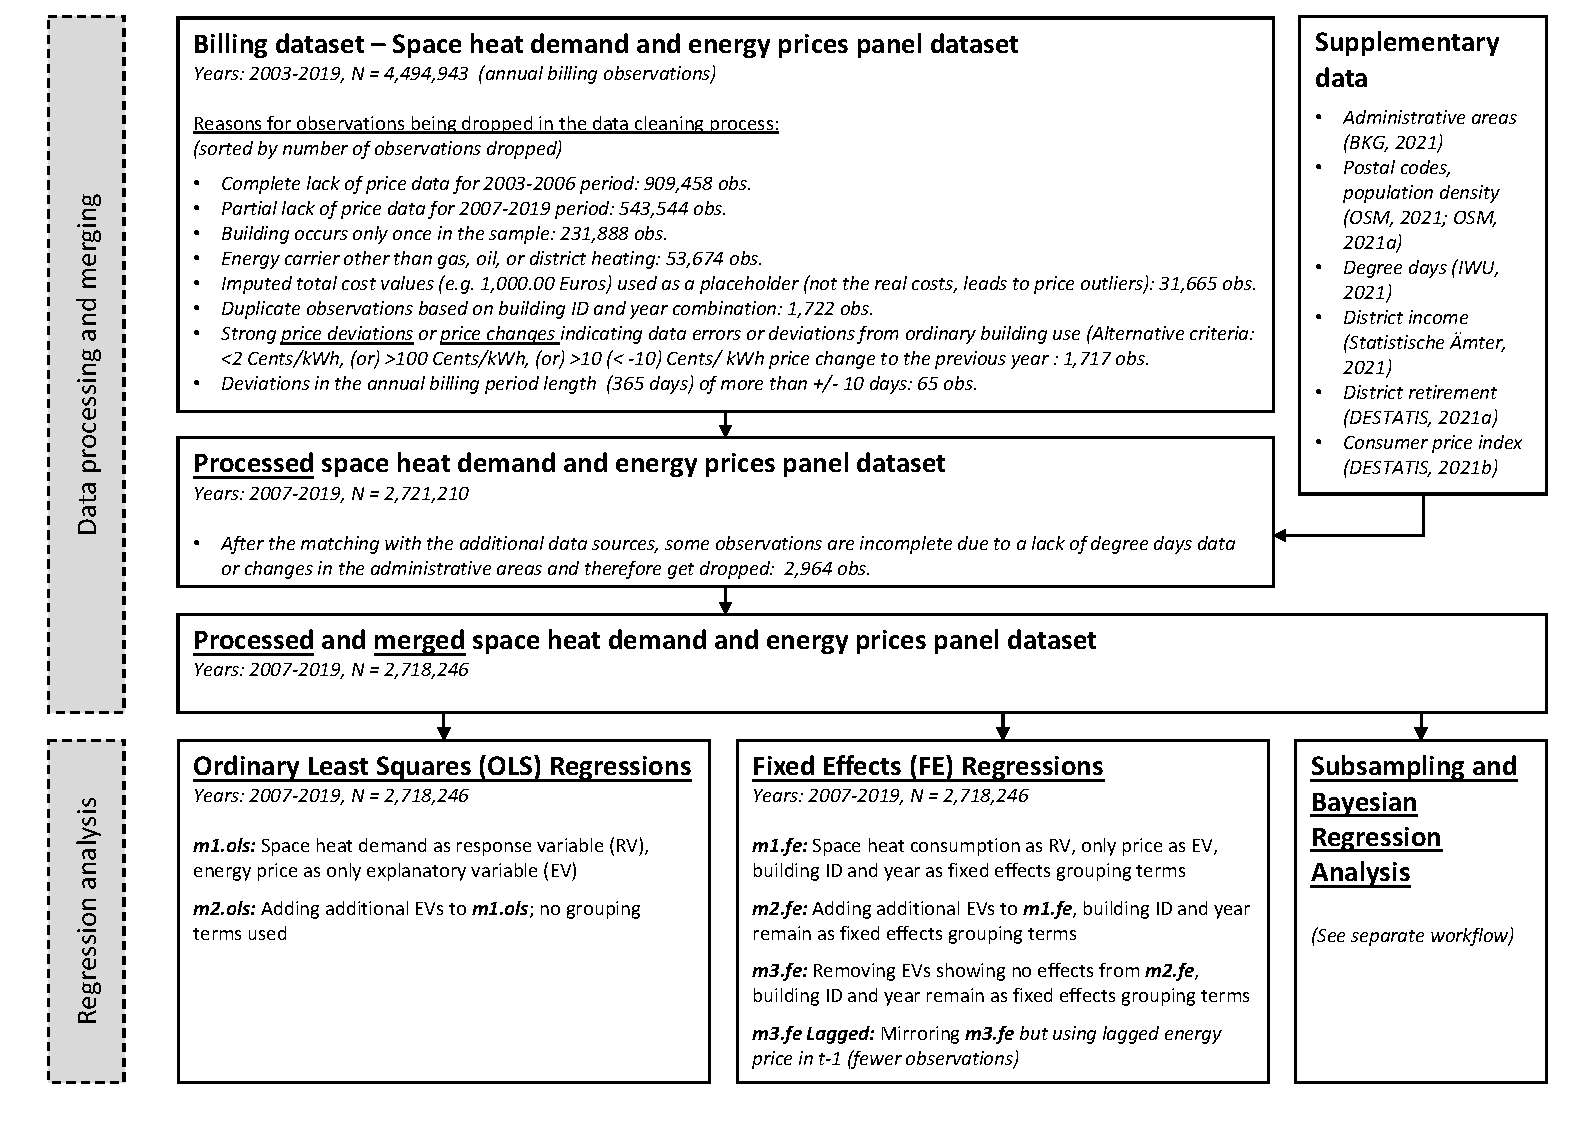
\includegraphics[width=1.03\linewidth]{figure/workflow_diagramm_part1} 

}

\caption{Workflow of data processing and regression analysis based on full sample}\label{fig:workflow1}
\end{figure}
The most important reason for exclusion from the sample is the absence of price data. In the period 2003-2006, price data are not available for any of the observations. This leads to the exclusion of 909,458 observations. In addition, price data are also missing for a part of the observations in the period 2009-2019. Due to these gaps in the price data, a further 543,544 observations are excluded from the dataset. A further 233,888 observations are removed from the sample because they are associated with buildings that occur only once in the sample. The decision to apply this criterion was mainly due to the fact that singular building IDs occurred mainly in the period 2007-2008, suggesting that IDs from this period are not linked with observations in later periods. Furthermore, observing a building at least twice during the analysed period allowed for cross-validation of matching building attributes and therefore better reliability of the data. Another 53,674 observations were removed from the sample because the buildings are heated with an energy carrier other than gas, oil, or district heating. Due to the small number of buildings compared to the total sample size and due to the heterogeneity of the group (both very modern buildings with heat pumps and un-renovated buildings with coal heating), it was decided to exclude all other energy carriers from the sample. In addition, another 1,722 observations were excluded as duplicates (matching building ID and year) and 65 observations due to a deviating length of the billing period (deviation of more than +/- 10 days).

In addition to the factors described above, there are two other reasons for excluding observations from the sample. Both reasons are related to outliers in the energy price data. Compared to the other cleaning steps described above, performing the analysis with and without these two steps in place has shown that they can have a strong effect on the results of the analysis and are therefore particularly important.

First, it was determined through exploratory testing and confirmed by ista that the price data contains fictitious cost values (e.g., 1,000.00 Euros for the entire building) that are used as placeholders and do not reflect actual costs. These fictitious cost values arise because ista, as a billing service provider, does not always have information about the costs incurred by the building owners and therefore uses the placeholders for internal technical reasons. The actual costs are only entered later by the building owners and therefore do not appear in the sample.\footnote{The internal practice of ista was reconstructed on the basis of an email exchange for the Wärmemonitor 2019, in which it was confirmed that the price data contain fictitious cost values.} This practice leads to the formation of outliers in the energy price data, as the fictitious cost values do not necessarily reflect the size and characteristics of a building. A total of 31,665 observations are removed due to fictitious cost values identified by searching for round cost rates without cent amounts that occur unusually often in the sample.

Second, despite the removal of the fictitious cost values, some spurious outliers remained in the price data. An exploratory review of individual cases revealed that the remaining price outliers were likely due to data errors (e.g., unrealistic heating areas), which is not unusual given the very large number of observations in the sample. Although a relatively small number, the price outliers can significantly interfere with the results of the analysis. Therefore, it was decided to also exclude the remaining observations that showed unrealistic deviations from the reasonable price level expected during the observation period (real prices: \textless2 cents/kWh or \textgreater100 cents/kWh) or large price changes from one period to another (real prices: \textgreater10 or \textless-10 cents/kWh compared to the previous year). The exclusion thresholds were based on expert judgments and were chosen to exclude only highly of implausible observations. Use of the thresholds resulted in the exclusion of an additional 1,717 observations from the sample.

The processed billing data are then matched with the external data sources (see figure \ref{fig:workflow1}). Due to missing degree days data or changes in the administrative areas, a further 1,940 observations are removed from the sample here, which ultimately leads to 2,719,270 remaining observations. After the processing, these observations are both complete and systematically checked for data errors that may have affected the outcome of the analysis.

\textbf{Regression analysis based on full sample}

{[}STILL MISSING{]}

\textbf{Stratified subsampling and Bayesian regression analysis}

{[}STILL MISSING{]}
\begin{figure}

{\centering 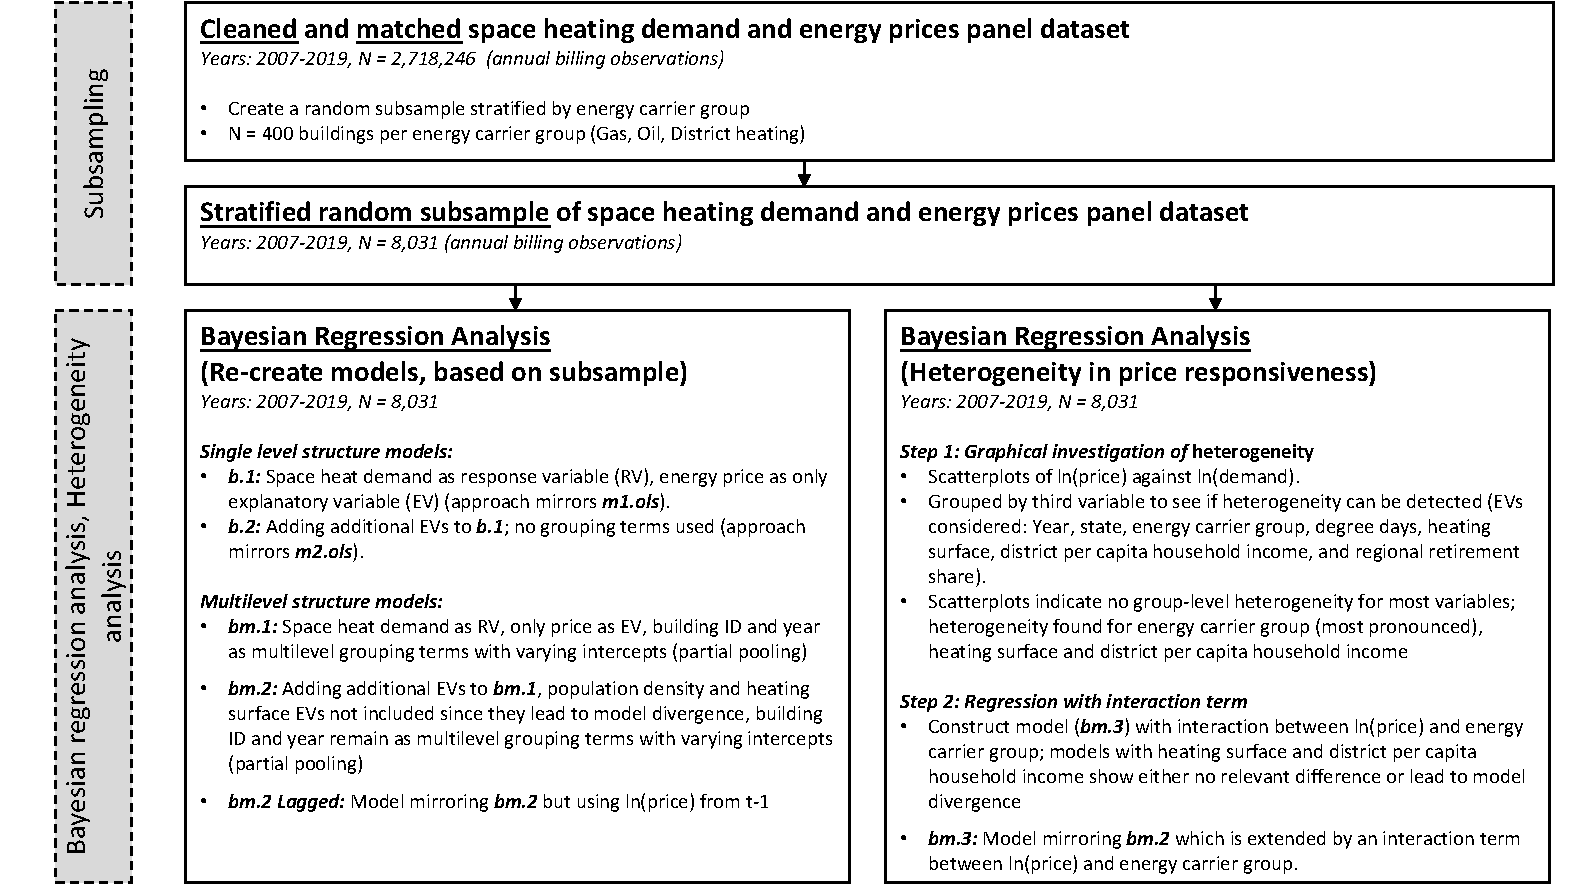
\includegraphics[width=1.03\linewidth]{figure/workflow_diagramm_part2} 

}

\caption{Workflow of stratified subsampling and Bayesian regression analysis based on subsample}\label{fig:workflow2}
\end{figure}
\hypertarget{descriptives}{%
\section{Descriptive statistics}\label{descriptives}}

\textbf{Unbalanced occurrence of buildings}

How often an individual building is observed in the processed and matched billing sample (full sample) is shown graphically in Figure \ref{fig:occurrence-buildings}. After excluding buildings that appeared only once in the sample (see Section \ref{workflow}), buildings are observed on average 6.77 times during the observation period. The histogram shows that not all buildings are observed throughout the whole observation period, leading to the panel being unbalanced. While a relatively large number of buildings are observed only twice, the distribution exhibits a second peak at nine and ten times observed. This means that information on a relevant proportion of the buildings in the sample is available almost throughout the entire observation period.
\begin{figure}

{\centering 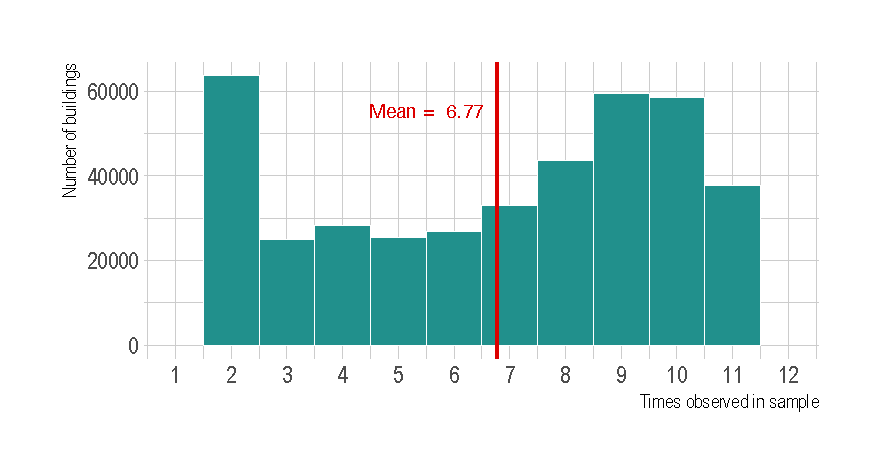
\includegraphics[width=0.75\linewidth]{figure/occurance_buildings} 

}

\caption{Number of occurrences of buildings in the full sample}\label{fig:occurrence-buildings}
\end{figure}
\textbf{Spatial and temporal coverage of sample}

In addition to how often an individual building is observed in the sample, also the spatial and temporal distribution of observations is of relevance. Figure \ref{fig:buildings-distribution} graphically depicts the spatial and temporal coverage of the full sample on the district-level.\footnote{Please note the use of the logarithmic scale in Figure \ref{fig:buildings-distribution}.} On the spatial dimension, the maps show that the coverage is good. There are very few districts without any building observed (transparent) and only a few districts with less than 10 buildings observed per year (dark blue). For most district-year combinations, more than 100 buildings are observed. In some large cities and metropolitan areas, numbers of more than 10,000 buildings annually are reached. The good spatial coverage of the data implies that results drawn from the sample have validity for Germany as a whole and are in their explanatory power not limited to certain regions or clusters.

On the temporal dimension, fewer observations are available in 2007 (43,696 observations) and 2008 (43,536 observations), as the energy price data was first included in these years. For the years between 2009 and 2019, an annual minimum of 201,856 and an average of 239,183 buildings are observed. Which means that the explanatory power of the results applies in particular to the period between 2009 and 2019. At the same time, exploratory testing of the data with and without consideration of the years 2007 and 2008 did not lead to a relevant change in the results meaning that the results are applicable to the whole time period under investigation.
\begin{figure}

{\centering 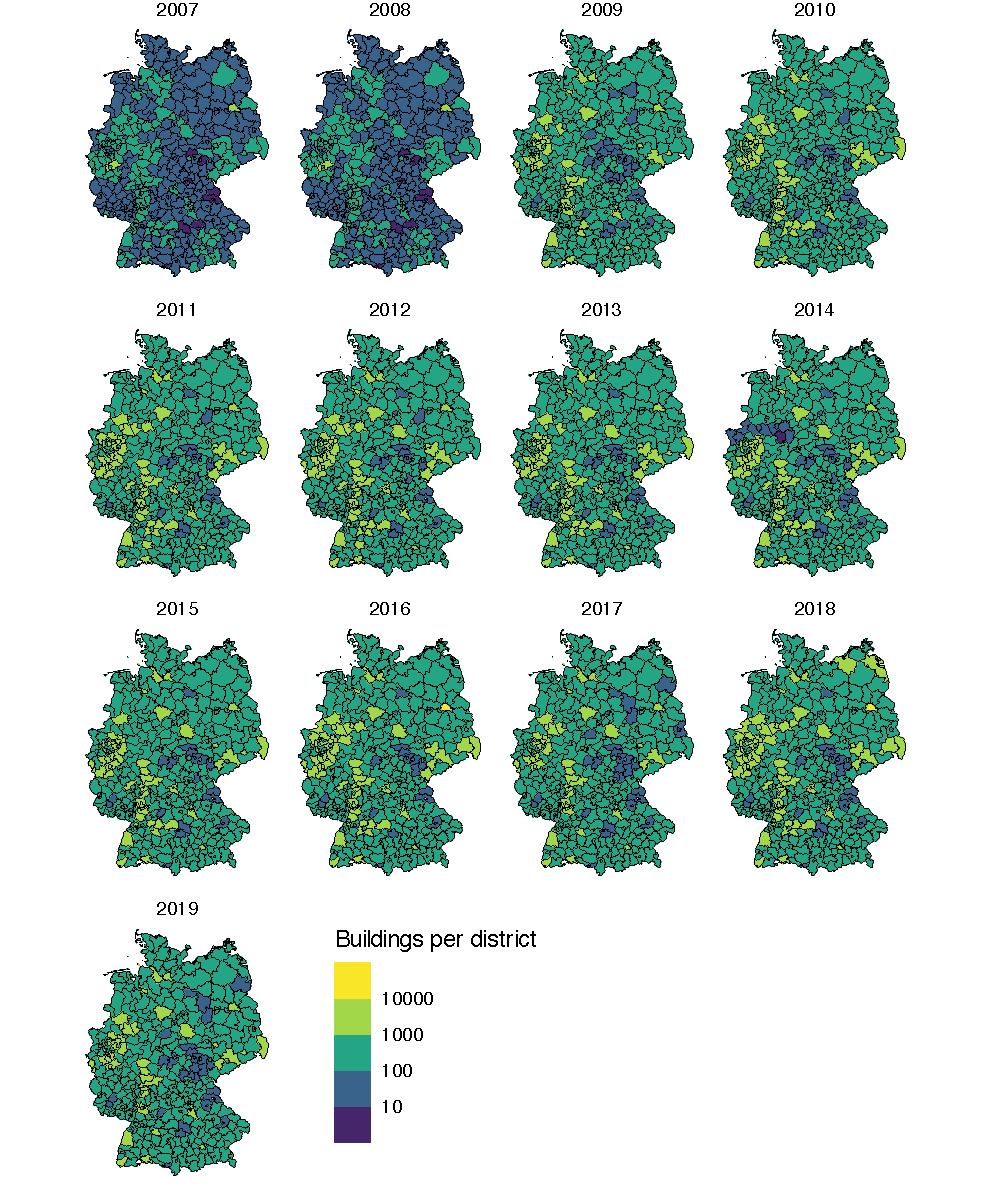
\includegraphics[width=0.77\linewidth]{figure/buildings_distribution} 

}

\caption{Spatial and temporal coverage by the buildings observed}\label{fig:buildings-distribution}
\end{figure}
\textbf{Summary statistics}

Table \ref{tab:summary-statistics} provides summary statistics for the full sample reporting the median values and the interquartile range (IQR). Besides the overall sample, also separate statistics for the three carrier types gas, oil, and district heating are included. About 60.6\% of the observations in the sample are associated with gas as the energy carrier. A further 29.5\% with oil and 9.9\% with district heating. For space heat demand, as the response variable, the median value (IQR) for the sample overall is 113 (86, 145) kWh/sqm/a and for energy price as the main explanatory variable the median (IQR) of the sample is 6.49 (5.77, 7.69) Cents/kWh.
\begin{table}[]
\centering
\caption{Summary statistics}
\label{tab:summary-statistics}
\resizebox{\textwidth}{!}{%
\begin{tabular}{@{}llllll@{}}
\toprule
Variable {[}Median (IQR){]} &
  Unit &
  \begin{tabular}[c]{@{}l@{}}Overall\\ N = 2,718,246\end{tabular} &
  \begin{tabular}[c]{@{}l@{}}Gas\\ N = 1,647,563 (60.6\%)\end{tabular} &
  \begin{tabular}[c]{@{}l@{}}Oil\\ N = 802,451 (29.5\%)\end{tabular} &
  \begin{tabular}[c]{@{}l@{}}District heating\\ N = 268,232 (9.9\%)\end{tabular} \\ \midrule
                                         &                 &                      &                      &                      &                      \\
Space heat demand, eff.                  & {[}kWh/sqm{]}   & 113 (86, 145)        & 116 (89, 149)        & 117 (91, 148)        & 83 (63, 109)         \\
Energy price, real                       & {[}Cents/kWh{]} & 6.49 (5.77, 7.69)    & 6.18 (5.56, 6.79)    & 7.06 (6.08, 8.25)    & 10.12 (8.71, 11.84)  \\
                                         &                 &                      &                      &                      &                      \\
Degree days                              &                 & 3,446 (3,214, 3,733) & 3,418 (3,192, 3,697) & 3,536 (3,273, 3,826) & 3,397 (3,191, 3,642) \\
Heating surface                          & {[}sqm{]}       & 404 (260, 707)       & 424 (271, 701)       & 305 (226, 466)       & 1,118 (556, 2,118)   \\
Housing units                            &                 & 6 (3, 10)            & 6 (3, 10)            & 4 (3, 6)             & 16 (8, 32)           \\
                                         &                 &                      &                      &                      &                      \\
\begin{tabular}[c]{@{}l@{}}District household income,\\ per capita\end{tabular} &
  {[}€/a{]} &
  20,695 (18,786, 22,568) &
  20,658 (18,731, 22,563) &
  21,098 (19,388, 22,861) &
  19,217 (17,667, 21,327) \\
District retirement share                & {[}\%{]}        & 0.207 (0.193, 0.220) & 0.209 (0.194, 0.222) & 0.205 (0.193, 0.216) & 0.210 (0.192, 0.230) \\
Postal code population density &
  \begin{tabular}[c]{@{}l@{}}{[}inhabitants/\\ sq. km{]}\end{tabular} &
  572 (217, 1,960) &
  662 (255, 2,121) &
  320 (149, 839) &
  2,053 (505, 4,821) \\ \midrule
\textit{Note: Median (IQR), No missings} &                 &                      &                      &                      &                      \\ \bottomrule
\end{tabular}%
}
\end{table}
In terms of energy demand and price, there are pronounced and relevant differences between the three types of energy carrier groups. The demand for gas and oil as energy carriers is higher than for district heating. The prices for gas are the lowest with relatively small fluctuations. Prices for oil are slightly higher, but show greater variation. Prices for district heating are by far the highest and also show the greatest variations. Additionally, buildings with a district heating system installed are three to four times the size of buildings with gas or oil heating installed (cf.~heating surface and housing units in Table \ref{tab:summary-statistics}).

\textbf{Focus on energy demand and prices}

Figure \ref{fig:demand-descriptive-graph} provides a more detailed visual summary of the demand variable. The aggregated demand distribution of the three carrier types and years tapers off towards the upper end. The lowest annual demands are around 25 kWh/sqm/a. The distribution peaks at just over 100 kWh/sqm/a and then tapers off to very high demand values of up to 350 kWh/sqm/a (Panel A). With a differentiated display by energy carrier (Panel B), the graph confirms the findings from Table \ref{tab:summary-statistics}. While the demands for gas and oil are on an almost similar higher level, demand in buildings with district heating is considerably lower. The major share of this difference in demand is most likely attributable to the difference in building size. Because buildings heated with district heating are on average three to four times larger than buildings with oil or gas heating, they have a better ratio of heating area to building exterior area, resulting in lower heat losses per square meter heated. Given the significance of the difference in demand, it was further scrutinized if the age of the building and the age of the heating system may deviate between gas and oil buildings on the one side and buildings with district heating on the other side. Newer buildings and newer heating systems would be expected to go along with lower energy demand. Appendix \ref{tab:age-building-heating-system} provides this comparison, which finds no differences between energy carriers of a magnitude that would suggest a strong impact on demand.
\begin{figure}

{\centering 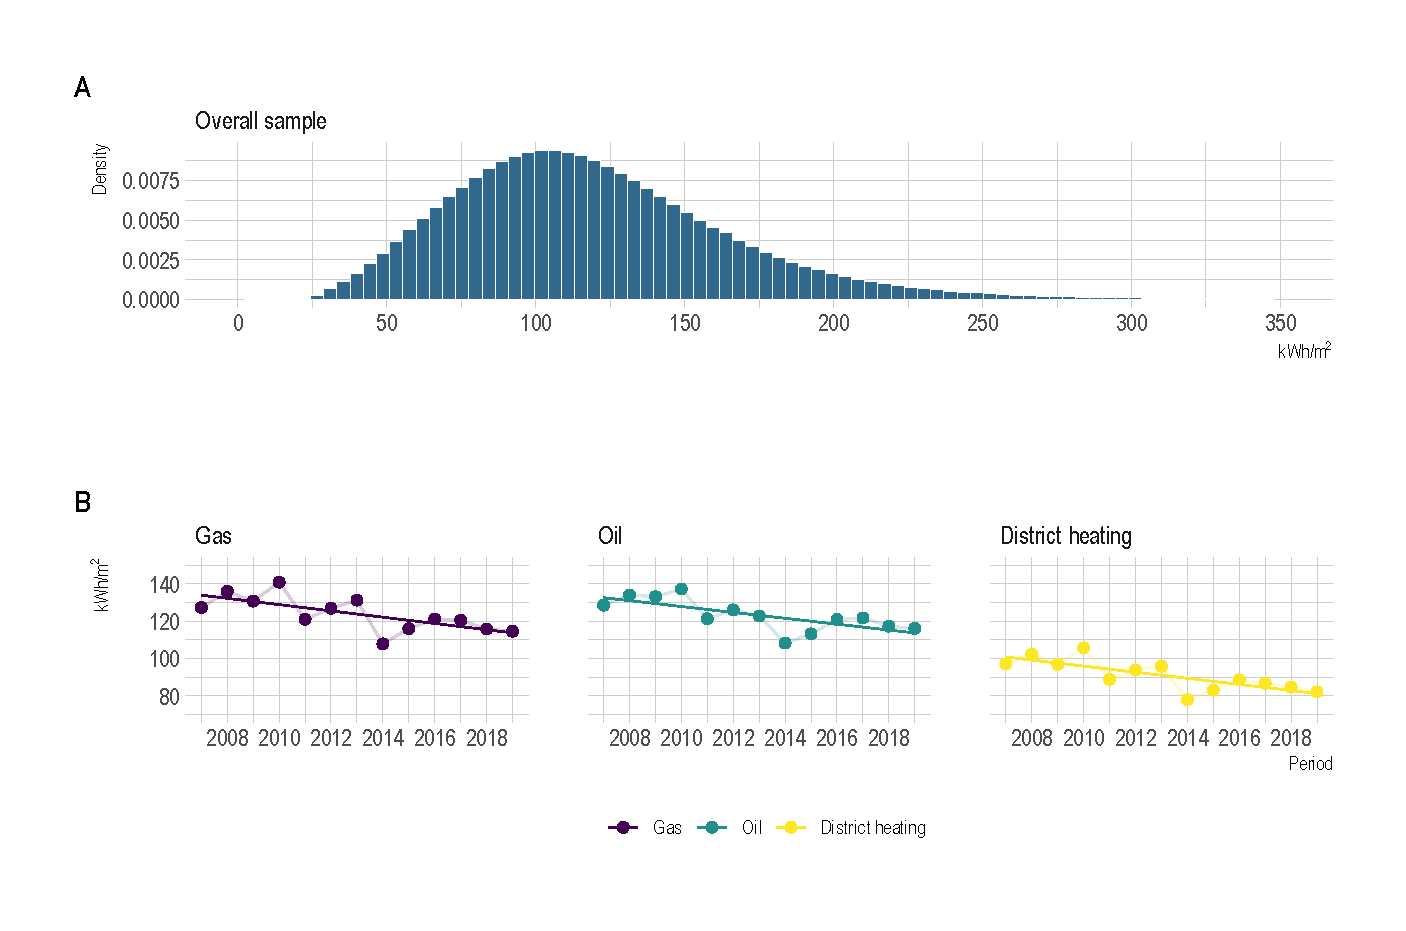
\includegraphics[width=1\linewidth]{figure/demand_descriptive} 

}

\caption{Distribution of energy demand}\label{fig:demand-descriptive-graph}
\end{figure}
In addition, Panel B of Figure \ref{fig:demand-descriptive-graph} provides two additional relevant pieces of information regarding the energy demand variable. First, for all three carrier types the effective demand decreases over time. This is most likely due to multiple factors one of which would be the demand response investigated in this thesis. Additionally, over time, newer more energy efficient buildings are added to the sample, while old and more inefficient building stock likely drops from the sample. Furthermore, the building stock remaining in the sample may undergo renovation measures leading to lower energy demand. Lastly, increasing outside temperatures due to climate change may also lead to the decline in effective demand observed. Linked to the role of climatic conditions is also a second aspect which can also be derived from the graph: Effective demand follows a similar pattern for all carriers, which can, however, also turn out to be higher or lower from year to year and only declines in the overall trend. Fluctuations in effective energy demand are linked to the variations in climatic conditions. In Appendix \ref{fig:degree-days-distribution} the distribution of degree days is depicted on a spatial and temporal scale. There is a consistent trend between degree days and energy demand that corroborates the intuition that higher degree days (lower outside temperatures) leads to higher energy demand. This illustrates the relevance of considering climatic conditions as an additional determinant of space heating demand.

Figure \ref{fig:price-descriptive-graph} depicts the distribution of nominal (Panel A) and real (Panel B) energy prices also by energy carrier. The points represent the average price in one year. The vertical bars represent the standard deviation. While the energy prices for gas are relatively stable over the period under observation, prices for oil show stronger volatility. As already established previously, prices for district heating are higher than those for gas and oil (cf.~Table \ref{tab:summary-statistics}). Furthermore, the prices for district heating are not as volatile, but show a huge range of variation, which is reflected in the much larger standard deviations.
\begin{figure}

{\centering 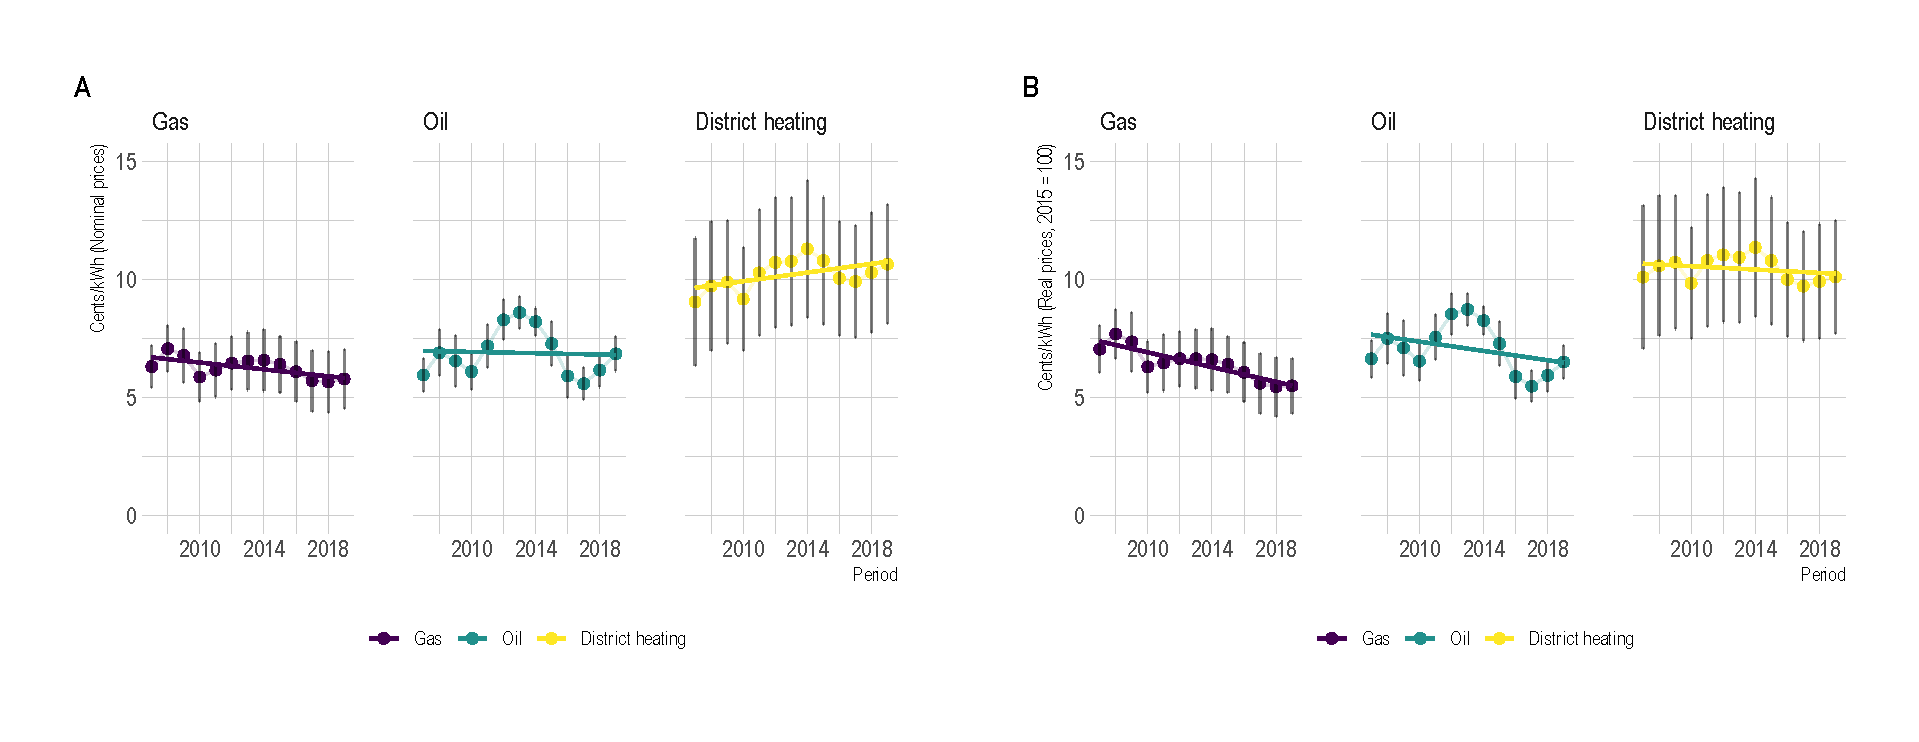
\includegraphics[width=1\linewidth]{figure/prices_descriptive} 

}

\caption{Distribution of nominal and real energy prices}\label{fig:price-descriptive-graph}
\end{figure}
While nominal prices are relatively stable in the overall trend for all three energy carrier groups, the trend changes after adjusting for inflation. The deflated real prices show an overall declining trend, with the trend being more pronounced for gas and oil. For the intuition about the price elasticity of space heating demand, this means that one would expect an overall increase in demand from the price effect alone. However, the graph also shows that effects into both directions can be observed when looking not at the overall trend but at year-to-year movements.

After having described the data and energy demand and energy prices as the two main variables in detail, the following section will present the results of the regression analysis.

\hypertarget{results}{%
\chapter{Results}\label{results}}

The results section is structured in two subsections. First, the results from the analysis of the full sample are presented (reflects first part of workflow, see Figure \ref{fig:workflow1}). And subsequently the results of the deepened analysis based on the stratified subsample are reported (reflects the second part of the workflow, see Figure \ref{fig:workflow2}).

\hypertarget{full_results}{%
\section{Full sample results}\label{full_results}}

In the
\begin{table}[]
\centering
\caption{Regression table for full sample analysis}
\label{tab:reg-table-full-sample}
\resizebox{\textwidth}{!}{%
\begin{tabular}{llrrrrrr}
\cline{3-8}
 &  & \multicolumn{6}{c}{Response variable in all model specifications: Ln of space heat demand} \\
 &  & \multicolumn{2}{c}{OLS regression} & \multicolumn{1}{c}{} & \multicolumn{3}{c}{Fixed Effects (FE) regression} \\
\multicolumn{1}{c}{} & \multicolumn{1}{c}{} & \multicolumn{1}{c}{(1)} & \multicolumn{1}{c}{(2)} & \multicolumn{1}{c}{} & \multicolumn{1}{c}{(3)} & \multicolumn{1}{c}{(4)} & \multicolumn{1}{c}{(5)} \\ \cline{1-1} \cline{3-4} \cline{6-8} 
(Intercept) &  & 5.399 *** & 3.593 *** &  &  &  &  \\
 &  & (0.002) & (0.028) &  &  &  &  \\
\begin{tabular}[c]{@{}l@{}}Ln of\\ energy price\end{tabular} &  & -0.365 *** & -0.365 *** &  & -0.251 *** & -0.243 *** & -0.243 *** \\
 &  & (0.001) & (0.001) &  & (0.001) & (0.001) & (0.001) \\
\begin{tabular}[c]{@{}l@{}}Ln of\\ degree days\end{tabular} &  &  & 0.626 *** &  &  & 0.779 *** & 0.779 *** \\
 &  &  & (0.002) &  &  & (0.003) & (0.003) \\
\begin{tabular}[c]{@{}l@{}}Ln of\\ heating surface\end{tabular} &  &  & -0.133 *** &  &  & -0.405 *** & -0.405 *** \\
 &  &  & (0.000) &  &  & (0.003) & (0.003) \\
\begin{tabular}[c]{@{}l@{}}Energy carrier:\\ Oil\end{tabular} &  &  & 0.031 *** &  &  & 0.097 *** & 0.097 *** \\
 &  &  & (0.001) &  &  & (0.002) & (0.002) \\
\begin{tabular}[c]{@{}l@{}}Energy carrier:\\ District heating\end{tabular} &  &  & -0.061 *** &  &  & -0.020 *** & -0.020 *** \\
 &  &  & (0.001) &  &  & (0.002) & (0.002) \\
\begin{tabular}[c]{@{}l@{}}Ln of\\ district income\end{tabular} &  &  & -0.277 *** &  &  & 0.022 ** & 0.022 ** \\
 &  &  & (0.002) &  &  & (0.008) & (0.008) \\
\begin{tabular}[c]{@{}l@{}}Ln of district\\ population density\end{tabular} &  &  & 0.043 *** &  &  & 0,000 &  \\
 &  &  & (0.000) &  &  & (0.005) &  \\
\begin{tabular}[c]{@{}l@{}}Ln of\\ retirement share\end{tabular} &  &  & -0.084 *** &  &  & 0.435 *** & 0.435 *** \\
 &  &  & (0.010) &  &  & (0.030) & (0.030) \\ \cline{1-1} \cline{3-4} \cline{6-8} 
N &  & 2718246 & 2718246 &  & 2718246 & 2718246 & 2718246 \\
R2 &  & 0,049 & 0,156 &  & 0,822 & 0,829 & 0,829 \\
logLik &  & -1322263,852 & -1159565,133 &  &  &  &  \\
AIC &  & 2644533,703 & 2319150,267 &  &  &  &  \\ \cline{1-1} \cline{3-4} \cline{6-8} 
\multicolumn{8}{l}{*** p \textless 0.001;  ** p \textless 0.01;  * p \textless 0.05.}
\end{tabular}%
}
\end{table}
\hypertarget{full_results}{%
\section{Subsample analysis}\label{full_results}}
\begin{figure}

{\centering 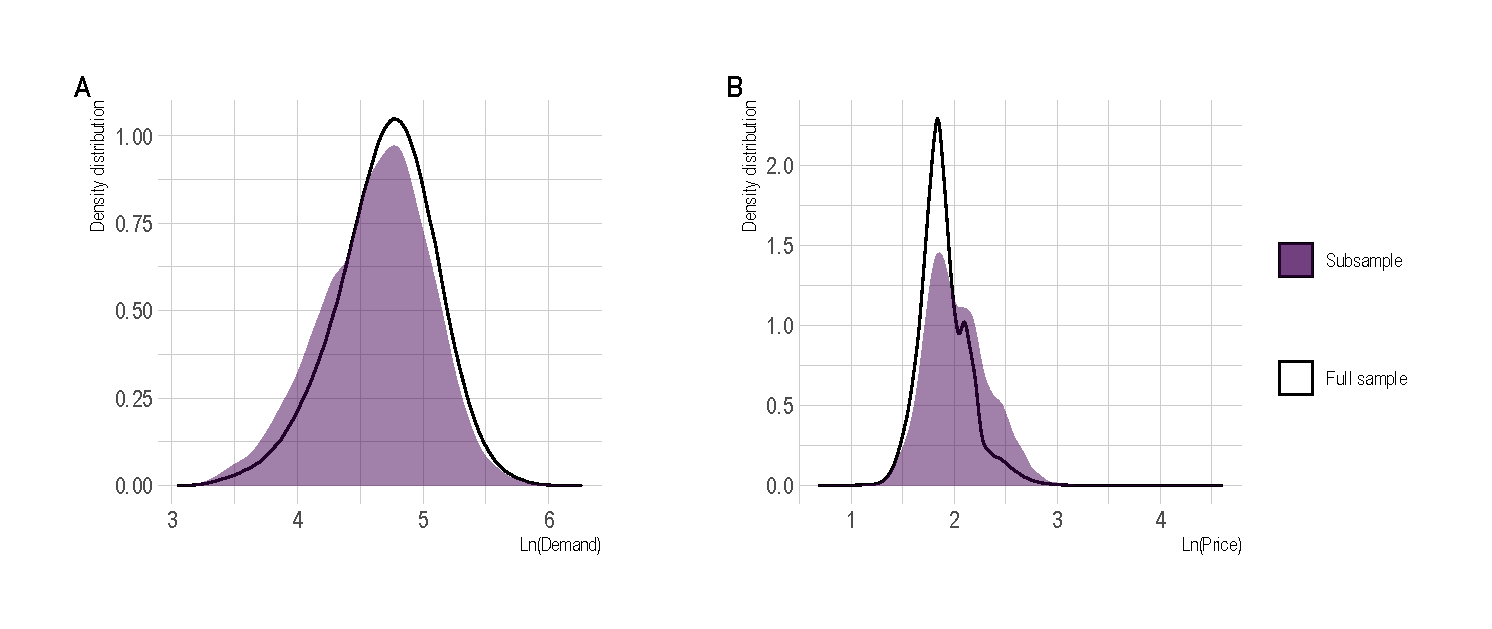
\includegraphics[width=1\linewidth]{figure/density-distribution-comparison-samples} 

}

\caption{Comparison of density distribution for energy demand and price between full sample and subsample}\label{fig:density-distribution-comparison-samples}
\end{figure}
\begin{figure}

{\centering 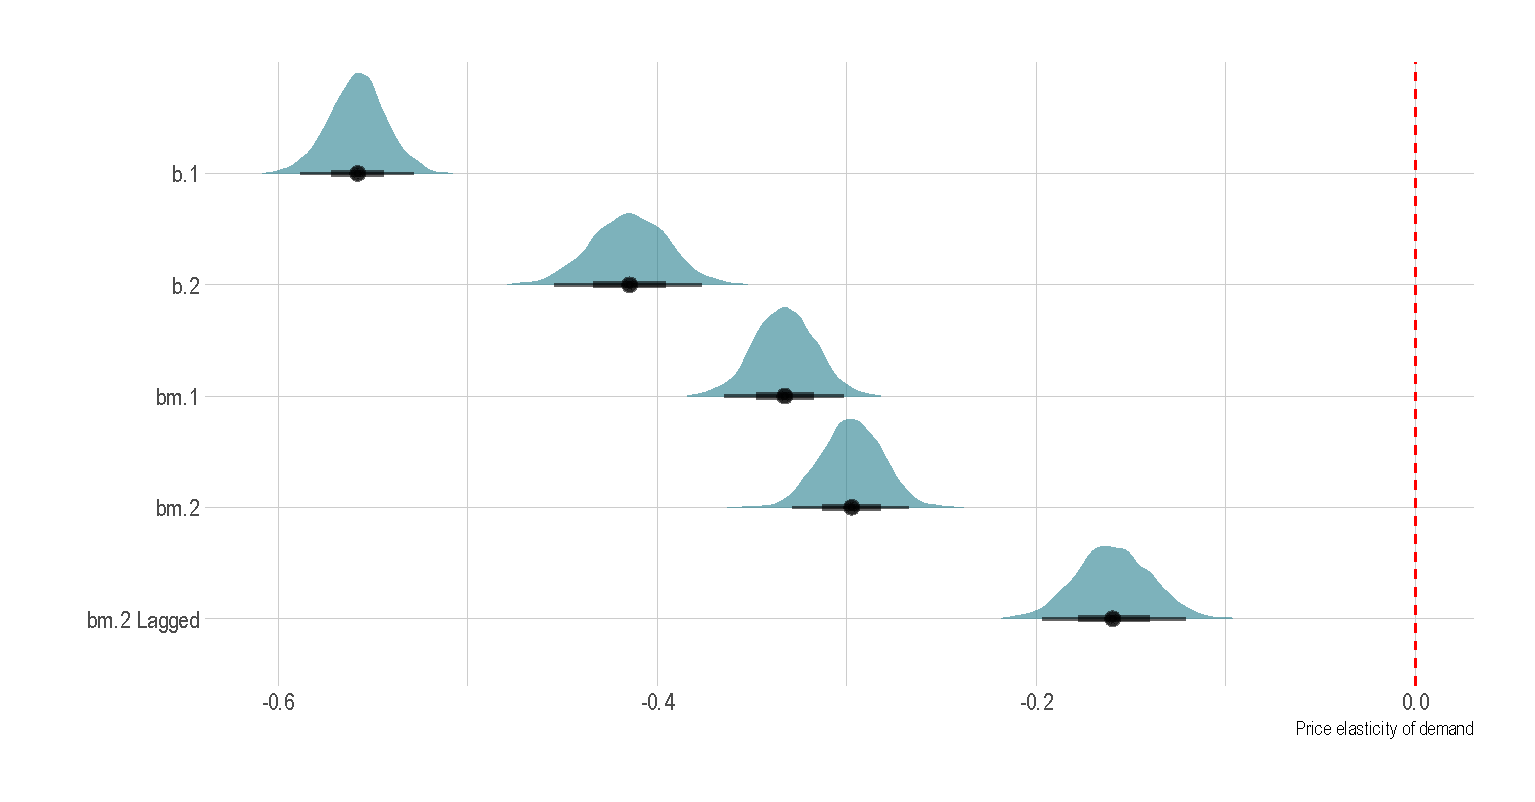
\includegraphics[width=1\linewidth]{figure/posterior-distributions} 

}

\caption{Posterior distributions for the price elasticities of space heating demand based on the subsample}\label{fig:posterior-distributions}
\end{figure}
\begin{figure}

{\centering 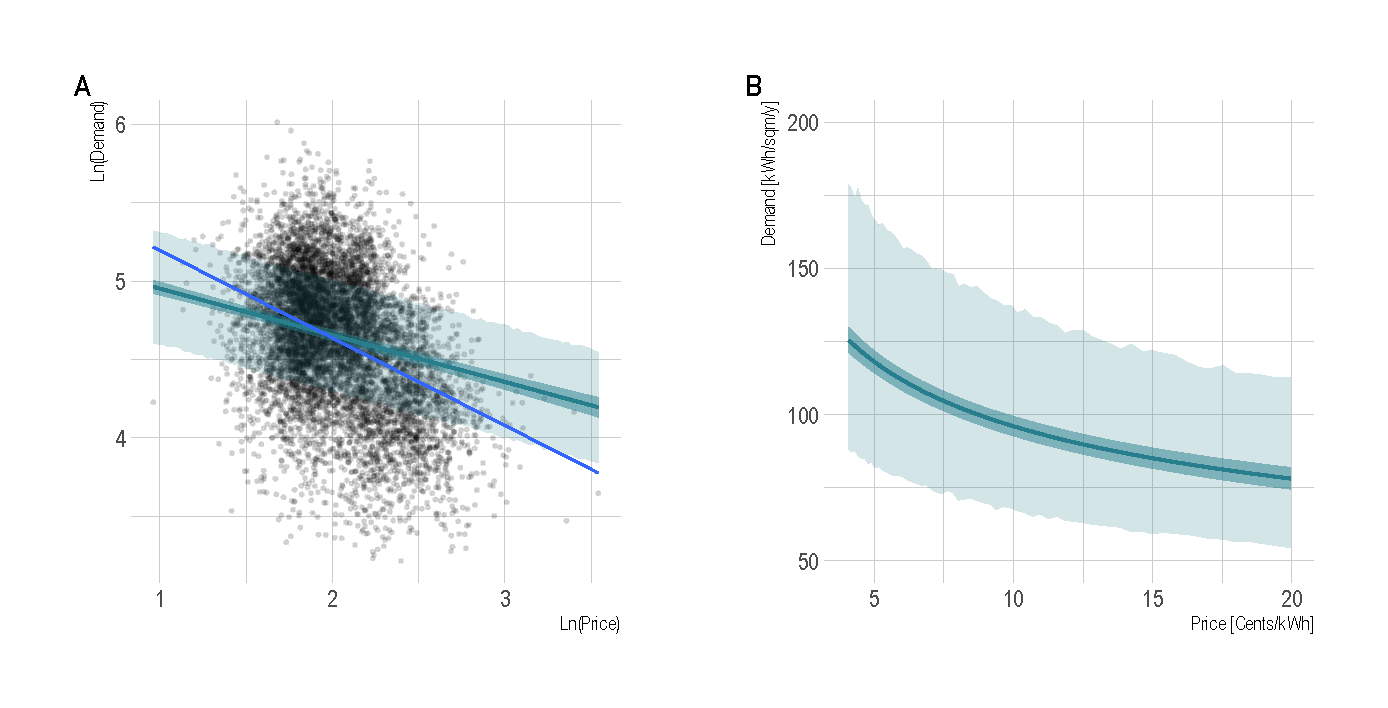
\includegraphics[width=1.04\linewidth]{figure/bm2_prediction} 

}

\caption{Predicted price elasticities of demand based on multilevel model}\label{fig:elasticity-predictions-bm2}
\end{figure}
\begin{figure}

{\centering 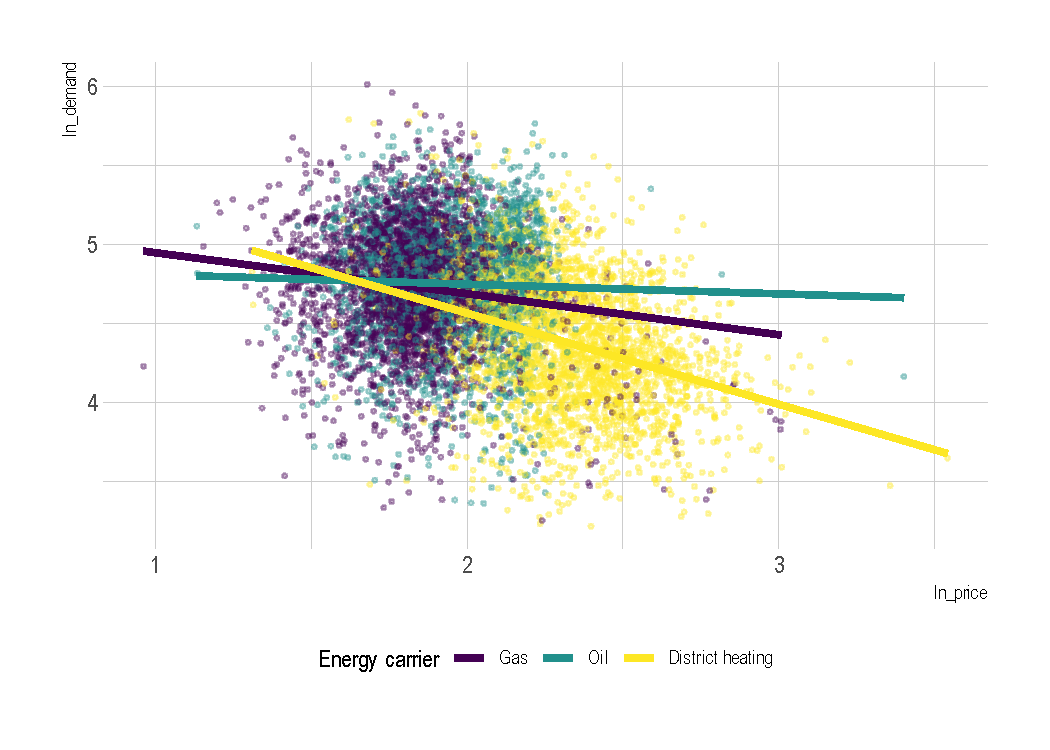
\includegraphics[width=1\linewidth]{figure/carrier_heterogeneity_plot} 

}

\caption{Investigation of heterogeneity between energy carrier groups}\label{fig:heterogeneity-energy-carrier-plot}
\end{figure}
\begin{figure}

{\centering 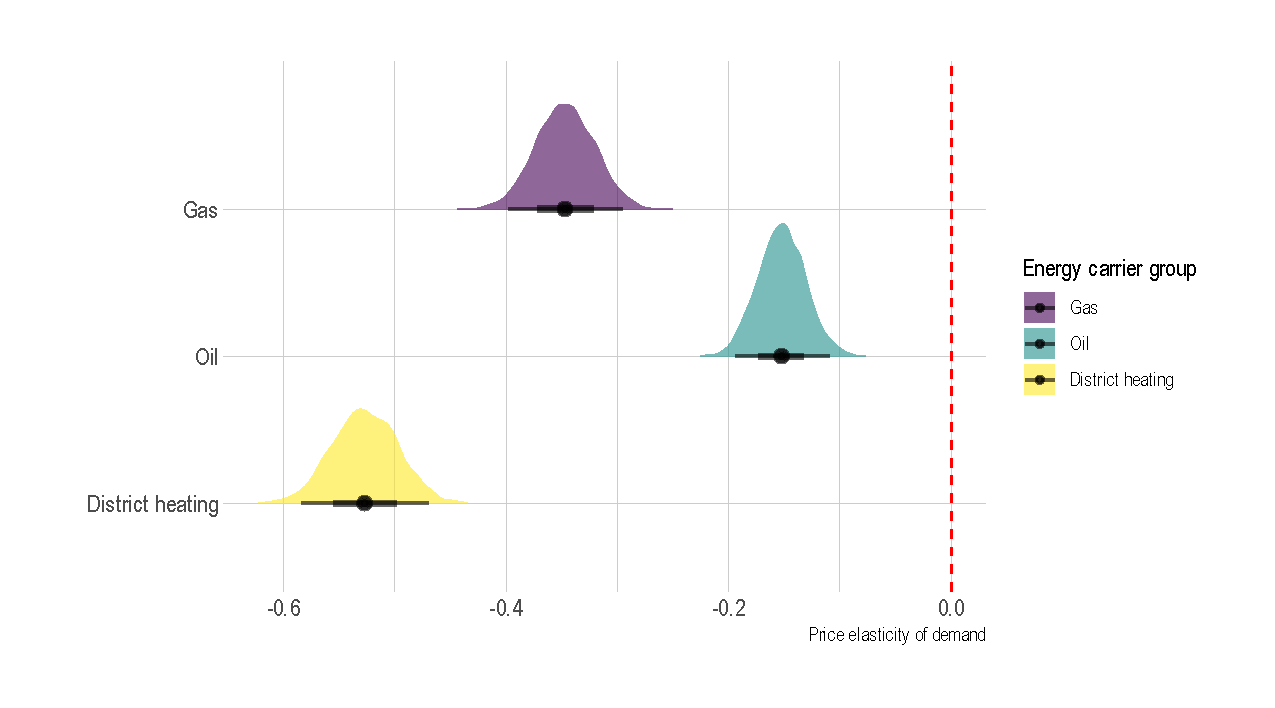
\includegraphics[width=1\linewidth]{figure/posterior-distribution-interaction} 

}

\caption{Posterior distributions for the price elasticities of space heating demand by energy carrier group based on the subsample}\label{fig:posterior-distribution-interaction}
\end{figure}
!!! Die nachfolgenden Tabellen müssen noch an neu durchgelaufenen Modelle angepasst werden
\begin{table}[]
\caption{Summary of coefficients for energy price in Bayesian models}
\label{tab:price-coefs-brms}
\resizebox{\textwidth}{!}{%
\begin{tabular}{@{}lllllllll@{}}
\toprule
Coef.                               & Model             & Estimate & Est.Error & l-95\% CI & u-95\% CI & Rhat & Bulk ESS & Tail ESS \\ \midrule
\multirow{5}{*}{Ln of energy price} & b.1               & -0.56    & 0.02      & -0.59     & -0.52     & 1    & 3165     & 2380     \\
                                    & b.2               & -0.50    & 0.02      & -0.54     & -0.46     & 1    & 3502     & 2521     \\
                                    & bm.1              & -0.30    & 0.02      & -0.34     & -0.25     & 1    & 1286     & 2114     \\
                                    & bm.2              & -0.25    & 0.02      & -0.29     & -0.20     & 1    & 2240     & 2742     \\
                                    & bm.2 - Renovation & -0.25    & 0.02      & -0.29     & -0.20     & 1    & 2184     & 2920     \\
Ln of energy price in t-1           & bm.2 - Price t-1  & -0.14    & 0.03      & -0.19     & -0.09     & 1    & 2326     & 2920     \\ \bottomrule
\end{tabular}%
}
\end{table}
\begin{table}[]
\centering
\caption{Model comparison based on PSIS-LOO}
\label{tab:model-comparison}
\begin{tabular}{@{}lrr@{}}
\toprule
     & \multicolumn{1}{l}{elpd\_diff} & \multicolumn{1}{l}{se\_diff} \\ \midrule
bm.3 & 0.0                            & 0.0                          \\
bm.2 & -14.7                          & 7.5                          \\
bm.1 & -90.3                          & 14.0                         \\
b.2  & -2856.7                        & 80.4                         \\
b.1  & -3100.5                        & 81.6                         \\ \bottomrule
\end{tabular}
\end{table}
\begin{figure}

{\centering 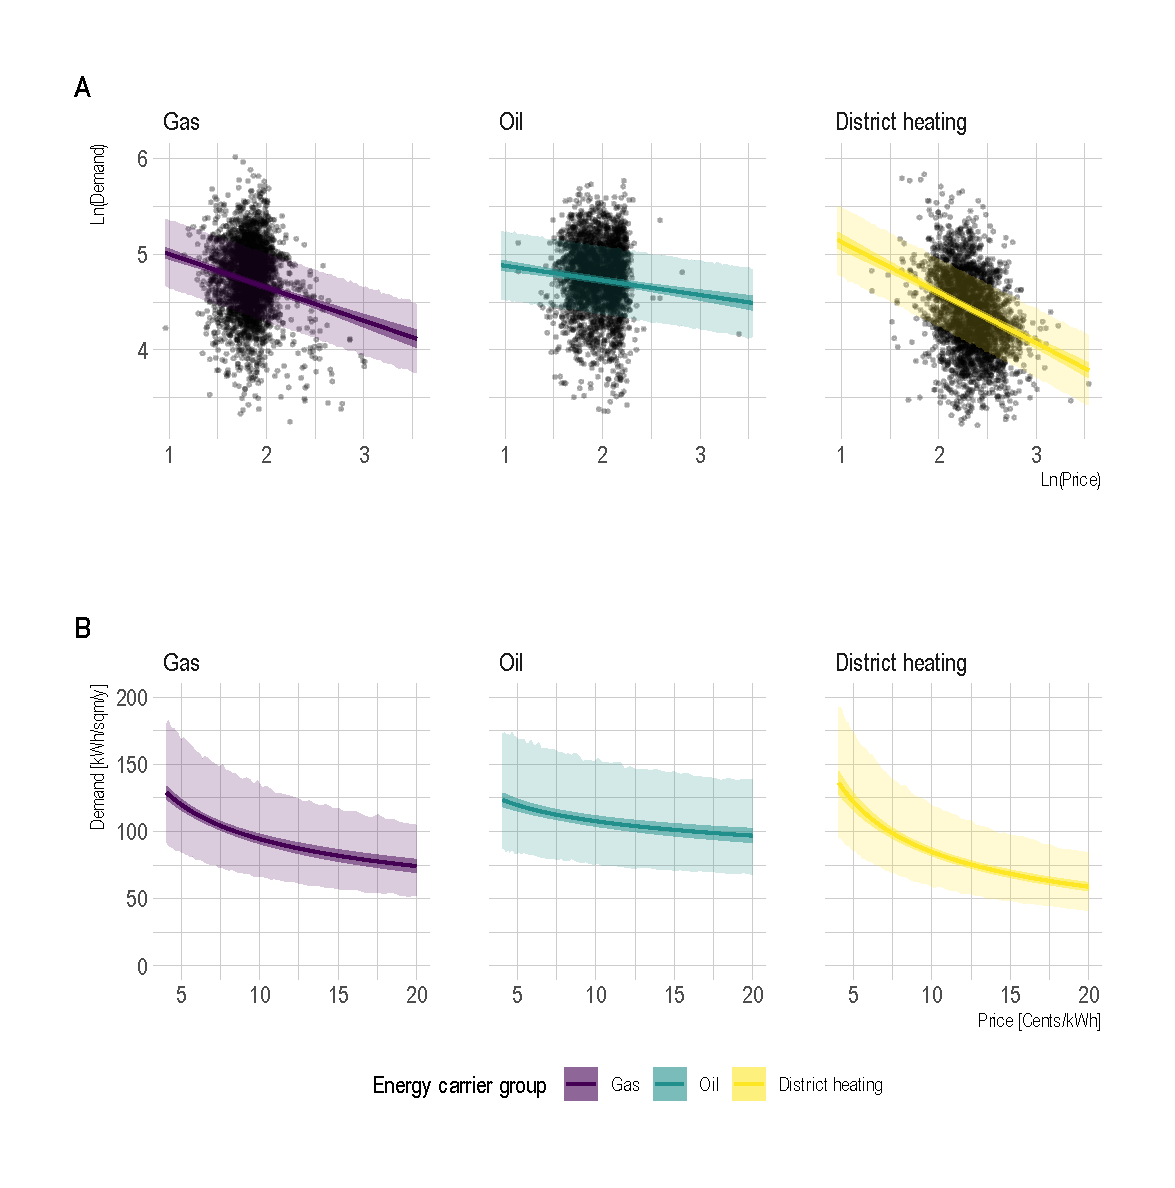
\includegraphics[width=1.04\linewidth]{figure/elasticity_predictions_subsample} 

}

\caption{Predicted price elasticities of demand by energy carrier group}\label{fig:elasticity-predictions-energy-carrier}
\end{figure}
Notes (copied from other papers):

-Accounting for unobserved heterogeneity reduces the elasticities by 15\% to 32\% relative to a model that does not include any effects at all, where the own price elasticity of electricity demand is −1.).

\hypertarget{discussion}{%
\chapter{Discussion}\label{discussion}}

NOTES - Energy taxation and climate change:
- Fuel consumption demand is determined by demand functions that depend primarily on income and prices
- Those who disfavor fuel taxes often claim they are strongly regressive. Earlier studies have shown that this depends on the country studied and on the details of the methods used, for instance if lifetime or temporary income is used, if substitution or other reactions are allowed for in the analysis. There is a tendency to progressivity in low income countries but regressivity in high income countries.
- Indirect channel of long-term price change and anticipation of those changes leading to investments in low-carbon UBA: Remediation measures drawn by lot through the BEHG are partly subsidized through the BEG or the tax incentive and are accounted for there (CO2 price as door opener for subsidy)

\hypertarget{discussion-of-elasticity-results}{%
\section{Discussion of elasticity results}\label{discussion-of-elasticity-results}}

\hypertarget{the-role-of-energy-prices-and-interaction-with-complementary-measures-policy-mix}{%
\section{The role of energy prices and interaction with complementary measures (policy-mix)}\label{the-role-of-energy-prices-and-interaction-with-complementary-measures-policy-mix}}
\begin{itemize}
\item
  For district heating larger share of costs are fixed; may drive the effect of larger price elasticities as data does not differentiate between fixed and variable cost components and with lower energy demand the per-unit cost rate increses due to the larger
\item
  Prices not the only option for action, potential overestimation of price relevance
\item
  Warmmietenmodell (Now only the renters are effected which will mainly trigger short-term price reactions; for decarbonisation need to tap the long-term channel; Lessors must be incentivized to initialize efficiency measures; one option: split prices but then long-term price signal is still partly muted; Warmmietmodell as an alternative where both parties renters and lessors have full economic incentive of pricing measures)
\end{itemize}
Relevance of Policy Mix - UBA (2022) study:
\begin{itemize}
\item
  Simulate the effect of various price paths for the BEHG until 2030 and simulate for the buildings sector (also consider the transportation and industry sector) how those varying price paths affect the level of sectoral emissions.
\item
  Shortcoming: They do not consider demand effects from price changes --\textgreater{} short-term effects that this theses argues for; prices are only endogenous effects on the long-term investment desicions.
\item
  Additional Shortcoming: Simulate choice of heat supply system, but not additional renovations, for example of the building envelope
\item
  With the findings from this thesis it must therefore be assumed that actual emissions would be lower than simulated in the model not considering demand adjustments from higher energy prices
\item
  Three scenarios: 1. BaU CO2 price of 125€/t in 2030; 2. Foresight, anticipation of energy prices for coming 5/10 yrs; 3. Foresight AND shorter lifetimes of heating systems (75\% of usual life-time) for increased replacement.
\item
  BaU: 86 Mt CO2e in 2030, KSG 2021 sector goal for buildings: 67 Mt CO2e in 2030; 28.4\% above the target
\item
  Only the scenarios with adjusted replacement rates + foresight meet or fall below the KSG (2021) targets (amended 2021 version).
\item
  Anticipation of higher CO2 prices over long time span has high impact; but effect about three times as large when combined with shorter lifetimes of heating systems
\item
  In scenarios with the assumption that heat supply systems are replaced more quickly due to the rising CO2 price, the heating replacement rate increases to around 5\%. In sensitivities in which no shorter lifetimes of the heat supply systems are assumed, the heating replacement rate is significantly lower.
\item
  Investitionsentscheidungen sind bedarfsgetrieben --\textgreater{} Policy Mix kann hier abhilfe Schaffen (bonus-malus system)
\item
  Another key finding is that significantly greater savings can be achieved if the capital good is replaced before the end of its respective service life. Due to the long-term capital stocks, the effects are greatest in the buildings and industry sectors, while in the transport sector the additional effect of early replacement is limited due to the comparatively short holding periods of vehicles.
\item
  Zusammenspiel: nur wenn fossile Investitionsgüter wirtschaftlich unattraktiv sind, wird durch die Austauschratenerhöhung die gewünschte Wirkung erzielt. Zusätzloiche Maßnahmen könnten sein: Verbesserung von Informationsverfügbarkeit, Ordnungsrecht oder finanzielle Förderungen. Besondere Bedeutung ist dabei einem verlässlich kommunizierten Preispfad des BEHG zuzumessen.
\item
  Das im Rahmen der aktuellen Beratungen zum Fit-for-55-Paket der EU zu erwartende verschärfte, neue ESR-Ziel wie auch die daraus abgeleitete neue BEHG-Höchstmenge wird in keiner CO2-Preissensitivität eingehalten.--\textgreater{} Einhaltung der ambitionierteren BEHG-Ziele höhere CO2-Preise als hier analysiert zu erwarten sind bzw. darüberhinausgehende klimapolitische Instrumente erforderlich sind
\item
  Damit bestätigt sich mit dieser Modellierungsarbeit auch die wirtschaftstheoretische Herleitung (vgl. Kemfert et al.~(2021)), dass zur Erreichung der Klimaschutzziele ein Politik-Mix zielführend ist, welcher die CO2-Bepreisung mit ordnungsrechtlichen Instrumenten, Förderprogrammen und weiteren Instrumenten (z.B. dem Abbau klimaschädlicher Subventionen) kombiniert.
\end{itemize}
\hypertarget{conclusion}{%
\chapter{Conclusion}\label{conclusion}}

\eqref{eq:ep}

\appendix

\hypertarget{supplementary-materials}{%
\chapter{Supplementary materials}\label{supplementary-materials}}

\singlespacing
\newpage
\begin{figure}

{\centering 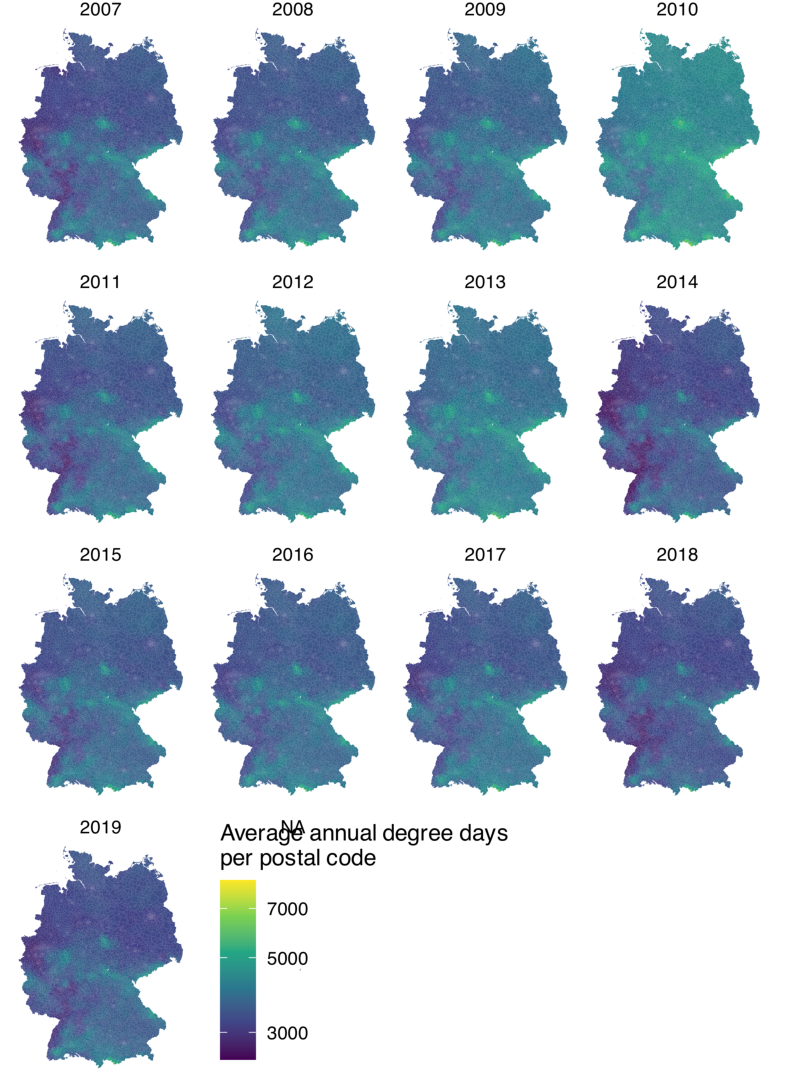
\includegraphics[width=0.77\linewidth]{figure/distribution_degree_days} 

}

\caption{Spatial and temporal variation in degree days}\label{fig:degree-days-distribution}
\end{figure}
\noindent
Figure \ref{fig:degree-days-distribution} show the spatial and temporal variation of outside temperature measured in degree days. Degree days data was taken from \protect\hyperlink{ref-iwu21}{IWU} (\protect\hyperlink{ref-iwu21}{2021}) and are used as an additional determinant of space heat demand in the regression analysis. Data is shown on the postal code level. Higher annual degree days are associated with lower temperatures and vice versa. In terms of spatial variation, the maps show cooler temperatures (higher degree days) mainly in the higher altitude regions, but also in eastern Germany, which is further inland from the European continent. In terms of temporal variation, 2010 in particular, but also 2012 and 2013 were cooler years than the average year in the sample. 2014, 2018 and 2019, on the other hand, were significantly warmer years.

\newpage
\begin{figure}

{\centering 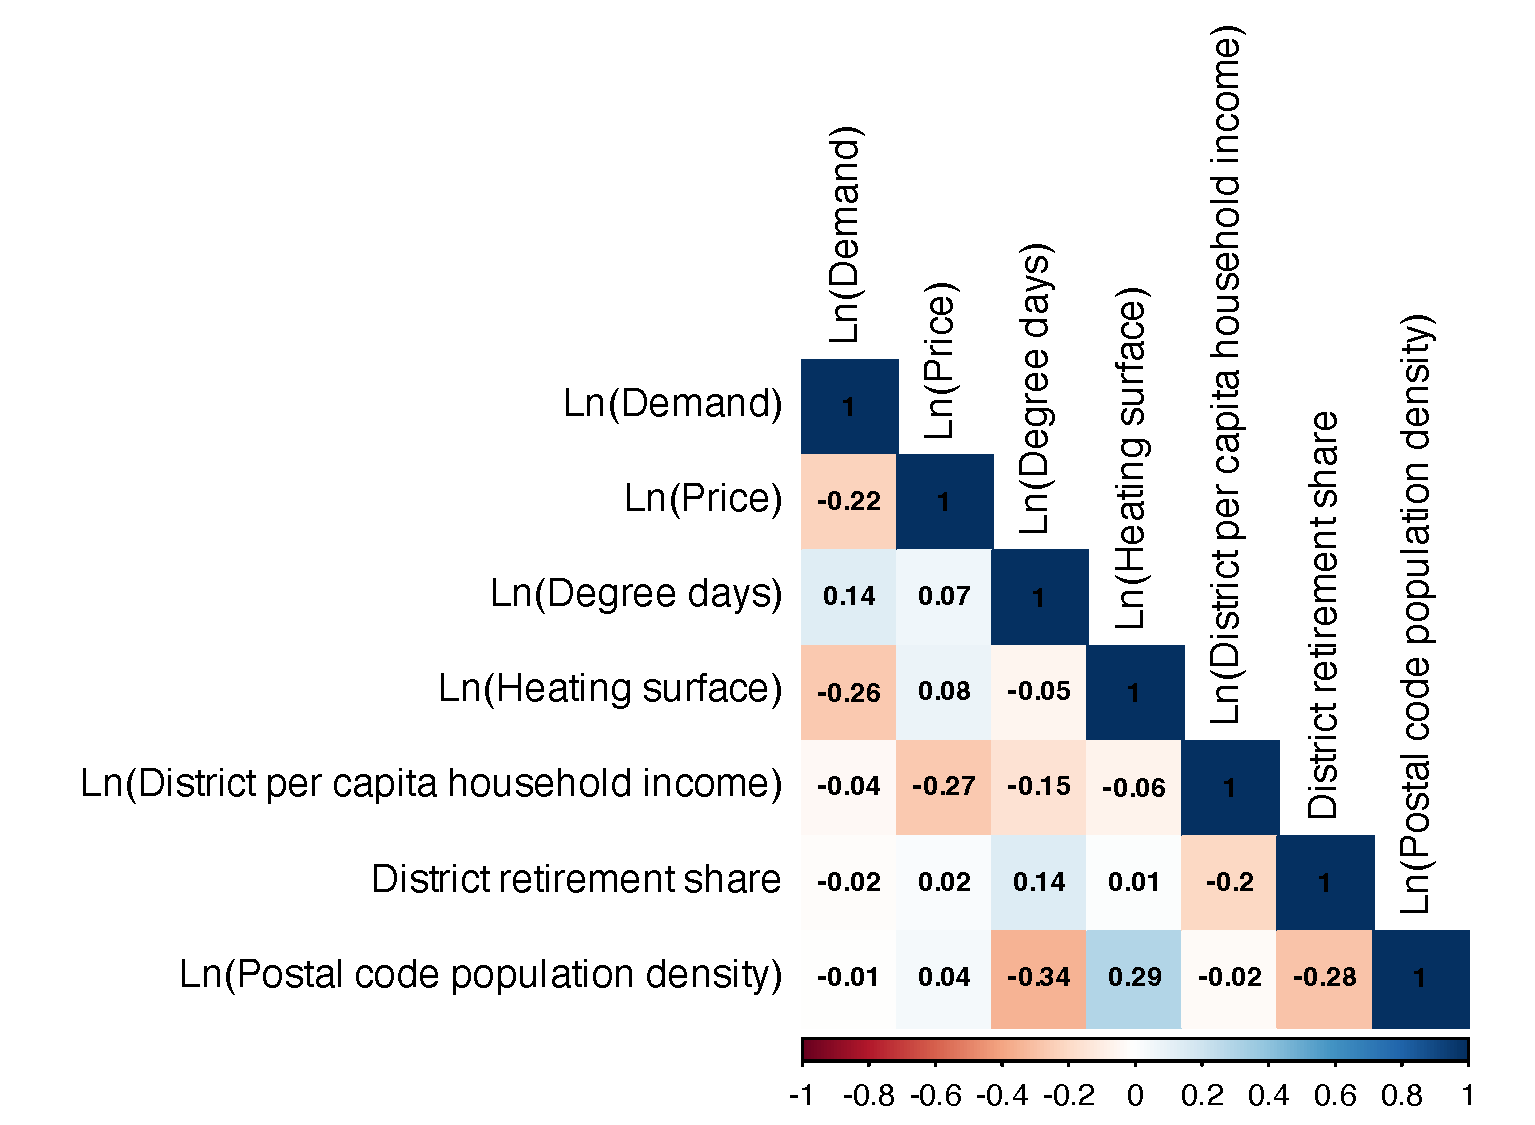
\includegraphics[width=0.9\linewidth]{figure/correlation_matrix} 

}

\caption{Pearson’s correlation matrix}\label{fig:correlation-plot}
\end{figure}
\noindent
The values in Figure \ref{fig:correlation-plot} represent Pearson's correlation coefficients. Values closer to 1 indicate a stronger positive relationship, values closer to -1 indicate a stronger negative relationship. Values close to zero indicate no relationship. None of the correlations observed between the variables exceed moderate values, ruling out possible multicollinearity issues. Energy price is negatively correlated with energy demand, indicating that the expected negative effect of price on demand indeed exists. Note that tall variables are ln-transformed.

\newpage
\begin{table}[]
\centering
\caption{Descriptive statistics for age of buildings and heating systems}
\label{tab:age-building-heating-system}
\resizebox{\textwidth}{!}{%
\begin{tabular}{@{}lllll@{}}
\toprule
Variable &
  \begin{tabular}[c]{@{}l@{}}Overall\\ N = 2,718,246\end{tabular} &
  \begin{tabular}[c]{@{}l@{}}Gas\\ N = 1,647,563\end{tabular} &
  \begin{tabular}[c]{@{}l@{}}Oil\\ N = 802,451\end{tabular} &
  \begin{tabular}[c]{@{}l@{}}District heating\\ N = 268,232\end{tabular} \\ \midrule
                                      &                    &                 &               &               \\
{\ul Building construction year}      &                    &                 &               &               \\
Until 1918                            & 34,536 (9.5\%)     & 22,004 (10.0\%) & 6,622 (6.1\%) & 5,910 (17\%)  \\
1919-1948                             & 22,652 (6.2\%)     & 14,494 (6.6\%)  & 4,742 (4.3\%) & 3,416 (9.7\%) \\
1949-1978                             & 121,949 (33\%)     & 68,253 (31\%)   & 42,973 (39\%) & 10,723 (30\%) \\
1979-1995                             & 126,299 (35\%)     & 76,869 (35\%)   & 40,072 (37\%) & 9,358 (26\%)  \\
1996-2009                             & 58,582 (16\%)      & 38,409 (17\%)   & 14,411 (13\%) & 5,762 (16\%)  \\
After 2010                            & 1,172 (0.3\%)      & 738 (0.3\%)     & 288 (0.3\%)   & 146 (0.4\%)   \\
(Missing)                             & 2,353,056          & 1,426,796       & 693,343       & 232,917       \\
                                      &                    &                 &               &               \\
\multicolumn{2}{l}{{\ul Heating system installation year}} &                 &               &               \\
Until 1978                            & 11,486 (3.5\%)     & 6,360 (3.2\%)   & 4,296 (4.5\%) & 830 (2.6\%)   \\
1979-1995                             & 118,401 (36\%)     & 71,848 (36\%)   & 36,359 (38\%) & 10,194 (32\%) \\
1996-2009                             & 151,172 (46\%)     & 93,734 (47\%)   & 41,161 (43\%) & 16,277 (51\%) \\
After 2010                            & 46,556 (14\%)      & 27,564 (14\%)   & 14,532 (15\%) & 4,460 (14\%)  \\
(Missing)                             & 2,390,631          & 1,448,057       & 706,103       & 236,471       \\
                                      &                    &                 &               &               \\ \midrule
\textit{Note: n (\%)}                 &                    &                 &               &               \\ \bottomrule
\end{tabular}%
}
\end{table}
\noindent
Table \ref{tab:age-building-heating-system} provides descriptive statistics for the age of buildings and heating systems grouped by the type of energy carrier. For those buildings, where information is available, a relatively larger share of district heating systems are installed in older buildings but at a more recent date. Overall, however, the differences are moderate and cannot explain the difference in energy demand between buildings with gas and oil heating on the one side (relatively higher consumption) and district heating on the other side (relatively lower consumption). Instead, it is presumably the size of the buildings that induces to the lower demand levels for buildings with district heating (cf.~Table \ref{tab:summary-statistics}. At the same time, it should be noted that the validity of the age classification of buildings and heating system installation year presented here is limited, as the information is available only for 15.5\% and 13.7\% of the total number of observations, respectively.

\newpage
\begin{table}[]
\centering
\caption{Comparison between full sample and sub-sample}
\label{tab:sample-comparison}
\resizebox{\textwidth}{!}{%
\begin{tabular}{@{}lllll@{}}
\toprule
Variable                                                                                       & Energy carrier group & \begin{tabular}[c]{@{}l@{}}Full sample\\ (N = 2.719.270)\end{tabular} & \begin{tabular}[c]{@{}l@{}}Sub-sample\\ (N = 4.410)\end{tabular} & Difference {[}\%{]}       \\ \midrule
\multirow{3}{*}{\begin{tabular}[c]{@{}l@{}}Energy demand\\ {[}kWh/m2{]}\end{tabular}}          & Gas                  & 122.5 {[}56.4; 209.33{]}                                              & 121.39 {[}55.4; 211.32{]}                                        & -0.91 {[}-1.81; 0.94{]}   \\
                                                                                               & Oil                  & 122.36 {[}58.67; 204{]}                                               & 116.97 {[}53.57; 198.17{]}                                       & -4.61 {[}-9.52; -2.94{]}  \\
                                                                                               & District heating     & 89.38 {[}43.23; 156.88{]}                                             & 83.98 {[}41.92; 141.01{]}                                        & -6.43 {[}-3.12; -11.25{]} \\
\multicolumn{5}{l}{} \\                                                                                                 
\multirow{3}{*}{\begin{tabular}[c]{@{}l@{}}Energy price, real \\ {[}Cents/kWh{]}\end{tabular}}        & Gas                  & 6.28 {[}4.56; 8.14{]}                                                 & 6.22 {[}4.59; 8.04{]}                                            & -0.96 {[}0.65; -1.24{]}   \\
                                                                                               & Oil                  & 7.14 {[}5.1; 9.18{]}                                                  & 7.21 {[}5.2; 9.23{]}                                             & 0.97 {[}1.92; 0.54{]}     \\
                                                                                               & District heating     & 10.45 {[}6.86; 15.07{]}                                               & 10.76 {[}7.17; 16.15{]}                                          & 2.88 {[}4.32; 6.69{]}     \\
\multicolumn{5}{l}{} \\   
\multirow{3}{*}{Degree days}                                                                   & Gas                  & 3467.6 {[}2921.14; 4180.42{]}                                         & 3461.14 {[}2914.56; 4180.4{]}                                    & -0.19 {[}-0.23; 0{]}      \\
                                                                                               & Oil                  & 3568.13 {[}2971.7; 4269.19{]}                                         & 3582.48 {[}2946.19; 4318.42{]}                                   & 0.4 {[}-0.87; 1.14{]}     \\
                                                                                               & District heating     & 3441.1 {[}2924.64; 4137.61{]}                                         & 3447.97 {[}2948.92; 4180.11{]}                                   & 0.2 {[}0.82; 1.02{]}      \\
\multicolumn{5}{l}{} \\   
\multirow{3}{*}{\begin{tabular}[c]{@{}l@{}}Building heating \\ surface {[}sqm{]}\end{tabular}} & Gas                  & 648.84 {[}163; 1849.4{]}                                              & 727.47 {[}168.04; 1817{]}                                        & 10.81 {[}3; -1.78{]}      \\
                                                                                               & Oil                  & 452.82 {[}160; 1195.6{]}                                              & 489.55 {[}167.1; 1362.8{]}                                       & 7.5 {[}4.25; 12.27{]}     \\
                                                                                               & District heating     & 1714.09 {[}255; 5030.18{]}                                            & 2034.55 {[}297.52; 6968.98{]}                                    & 15.75 {[}14.29; 27.82{]}  \\ \midrule
\multicolumn{5}{l}{\textit{*) Mean {[}90\% CI{]}}}                                                                                                                                                                                                                                          
\end{tabular}%
}
\end{table}
\noindent
Table \ref{tab:sample-comparison} compares the total sample and the sub-sample with respect to key variables. It contains the mean values for the two samples and the lower and upper limits of a 90\% interval divided by the energy carrier. It also gives the relative difference between the total sample and the sub-sample in percent. The statistics show that in the sub-sample with the available epc information, the buildings are on average 7.5 \% to 15.8 \% larger, depending on the energy carrier. This deviation is presumably due to the fact that larger buildings are more often managed by larger property managers who decide to systematically exchange their information with ista and also obtain their energy performance certificates through this standardised channel. The larger building heating area is likely also the reason for the deviations between the total sample and the sub-sample in energy demand for oil (-4.6\%) and district heating (-6.4\%). However, the deviations are within reasonable limits. Energy price and degree days from both samples are in good agreement.

\newpage
\begin{figure}

{\centering 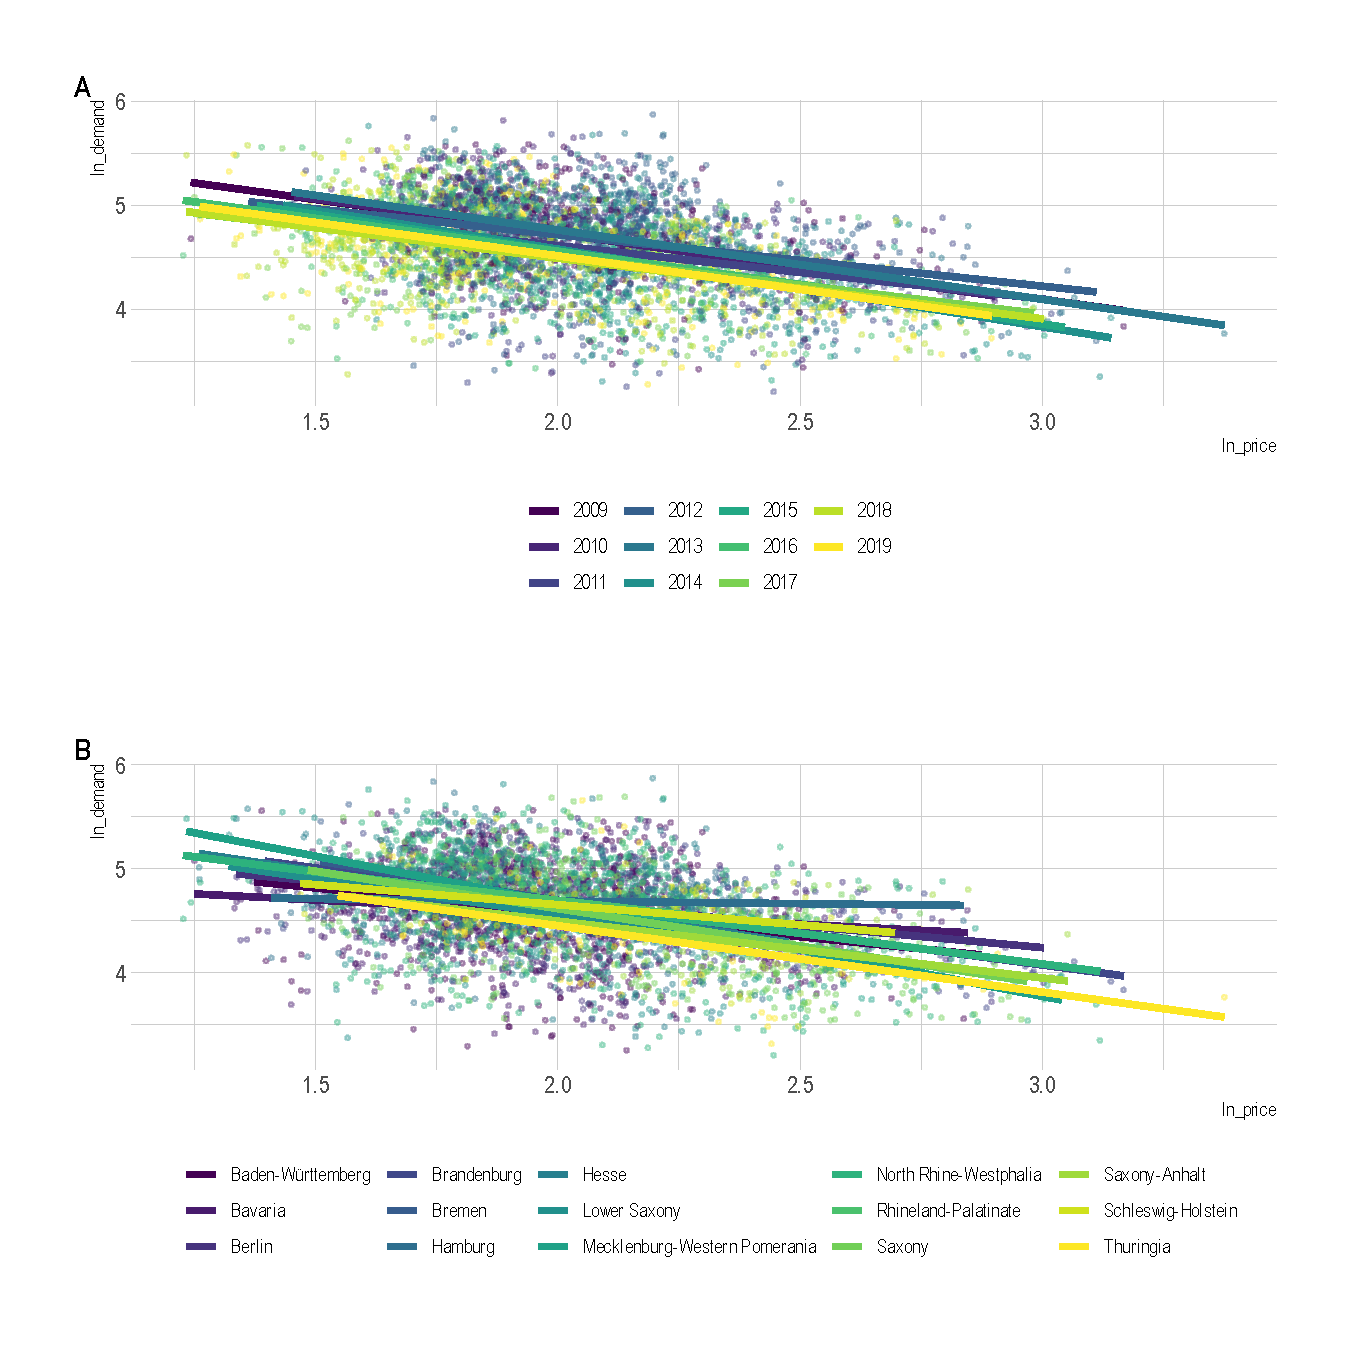
\includegraphics[width=1\linewidth]{figure/year_state_heterogeneity_plot} 

}

\caption{Investigation of heterogeneity for years and federal states}\label{fig:heterogeneity-year-state-plot}
\end{figure}
\noindent
Figure \ref{fig:heterogeneity-year-state-plot} presents a visual examination of the heterogeneity of price elasticity between years (Panel A) and federal states (Panel B). For this purpose, the observations in the sub-sample are grouped by year/federal state and presented in a scatter plot. The lines in the diagrams reflect simple linear models for the years/federal states as groups. Between years, all lines are almost parallel, indicating that there is no relevant difference in price elasticity between years. For the federal states, the lines scatter a little. At the same time, however, no strong pattern can be discerned through clusters such as differences between formerly eastern and western federal states or through other regional clusters.

\newpage
\begin{figure}

{\centering 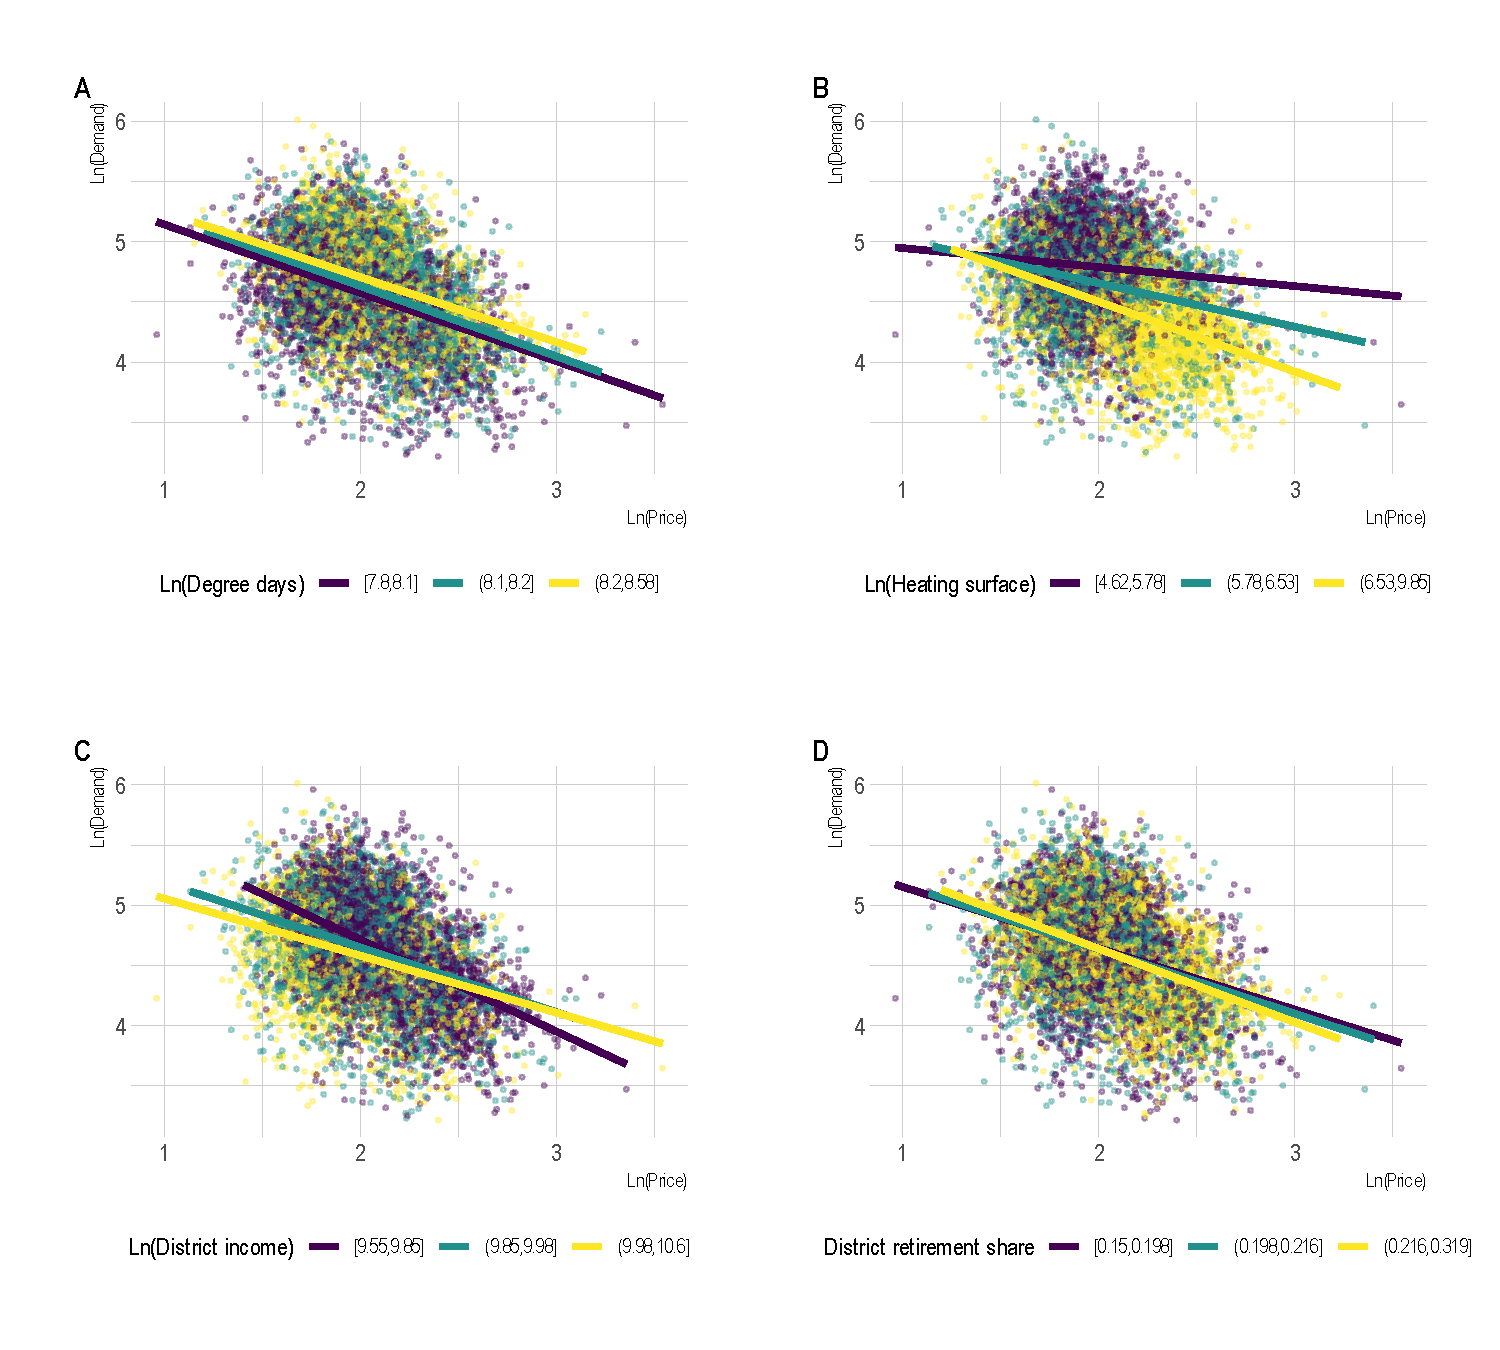
\includegraphics[width=0.95\linewidth]{figure/other_variables_heterogeneity_plot} 

}

\caption{Investigation of heterogeneity for degree days, heating surface, district income, and district retirement share}\label{fig:other-variables-heterogeneity-plot}
\end{figure}
\noindent
Figure \ref{fig:other-variables-heterogeneity-plot} presents a visual examination of the heterogeneity of price elasticity for the four variables degree days (Panel A), building heating surface (Panel B), average district income (Panel C), and district retirement share (Panel D). Since all four variables represent continuous variables, observations in the sub-sample are ln-transformed, grouped into three equally sized groups,\footnote{E.g., one third of observations with lowest number of degree days (between 7.85 and 8.1), one third of observations medium number of degree days (between 8.1 and 8.2), and one third of observations highest number of degree days (between 8.2 and 8.63).} and presented in a scatter plot. The lines in the diagrams reflect simple linear models for the respective three groups of equal size. For degree days, the lines are almost parallel and show no difference in price elasticity. For the other three variables, a slight dispersion of the grouped lines can be observed. But again, there are no pronounced differences that would prompt a more detailed investigation.

\newpage
\begin{figure}

{\centering 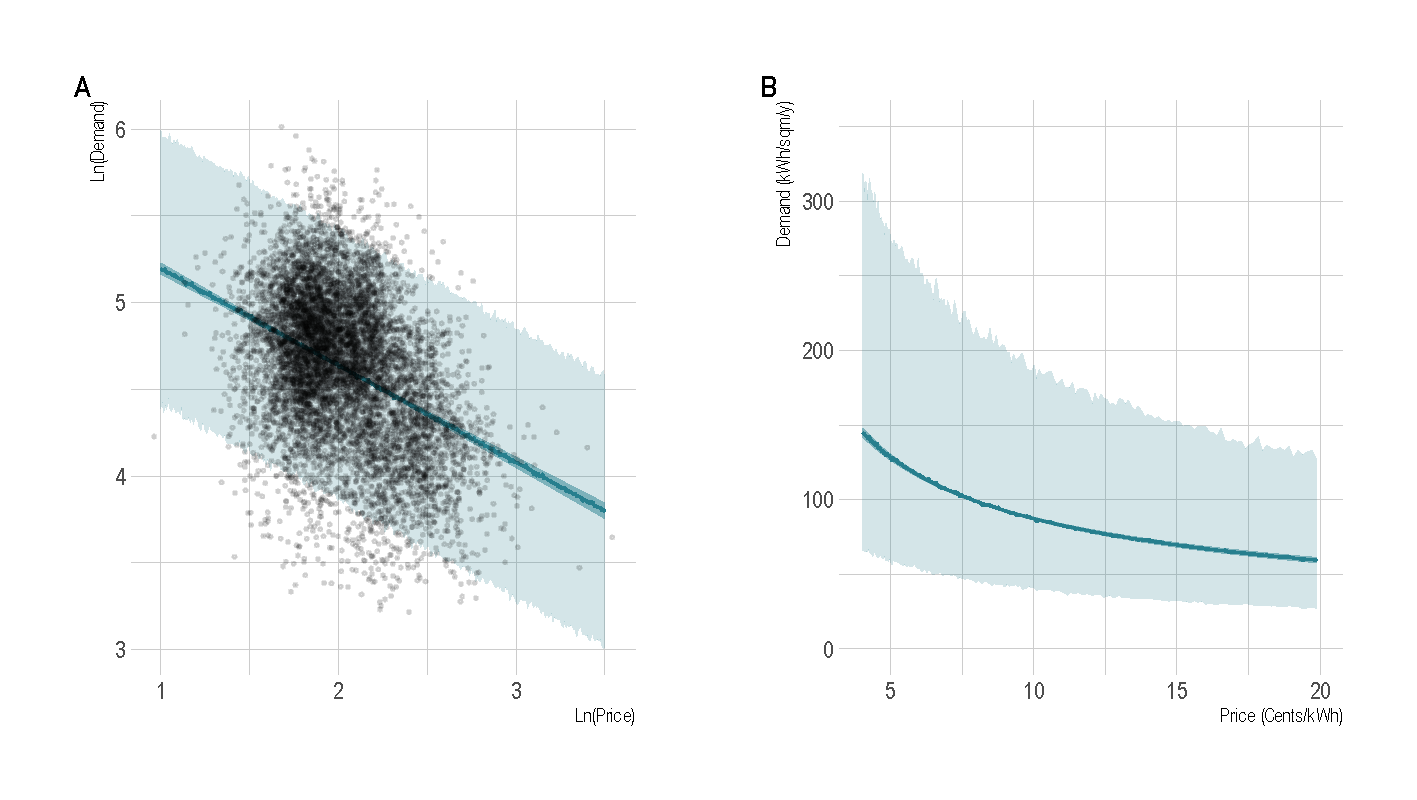
\includegraphics[width=1\linewidth]{figure/b1_prediction} 

}

\caption{Predicted price elasticities of demand based on price as only predictor}\label{fig:elasticity-predictions-b1}
\end{figure}
\noindent
Figure \ref{fig:elasticity-predictions-b1} presents (\ldots)

\newpage
\begin{figure}

{\centering 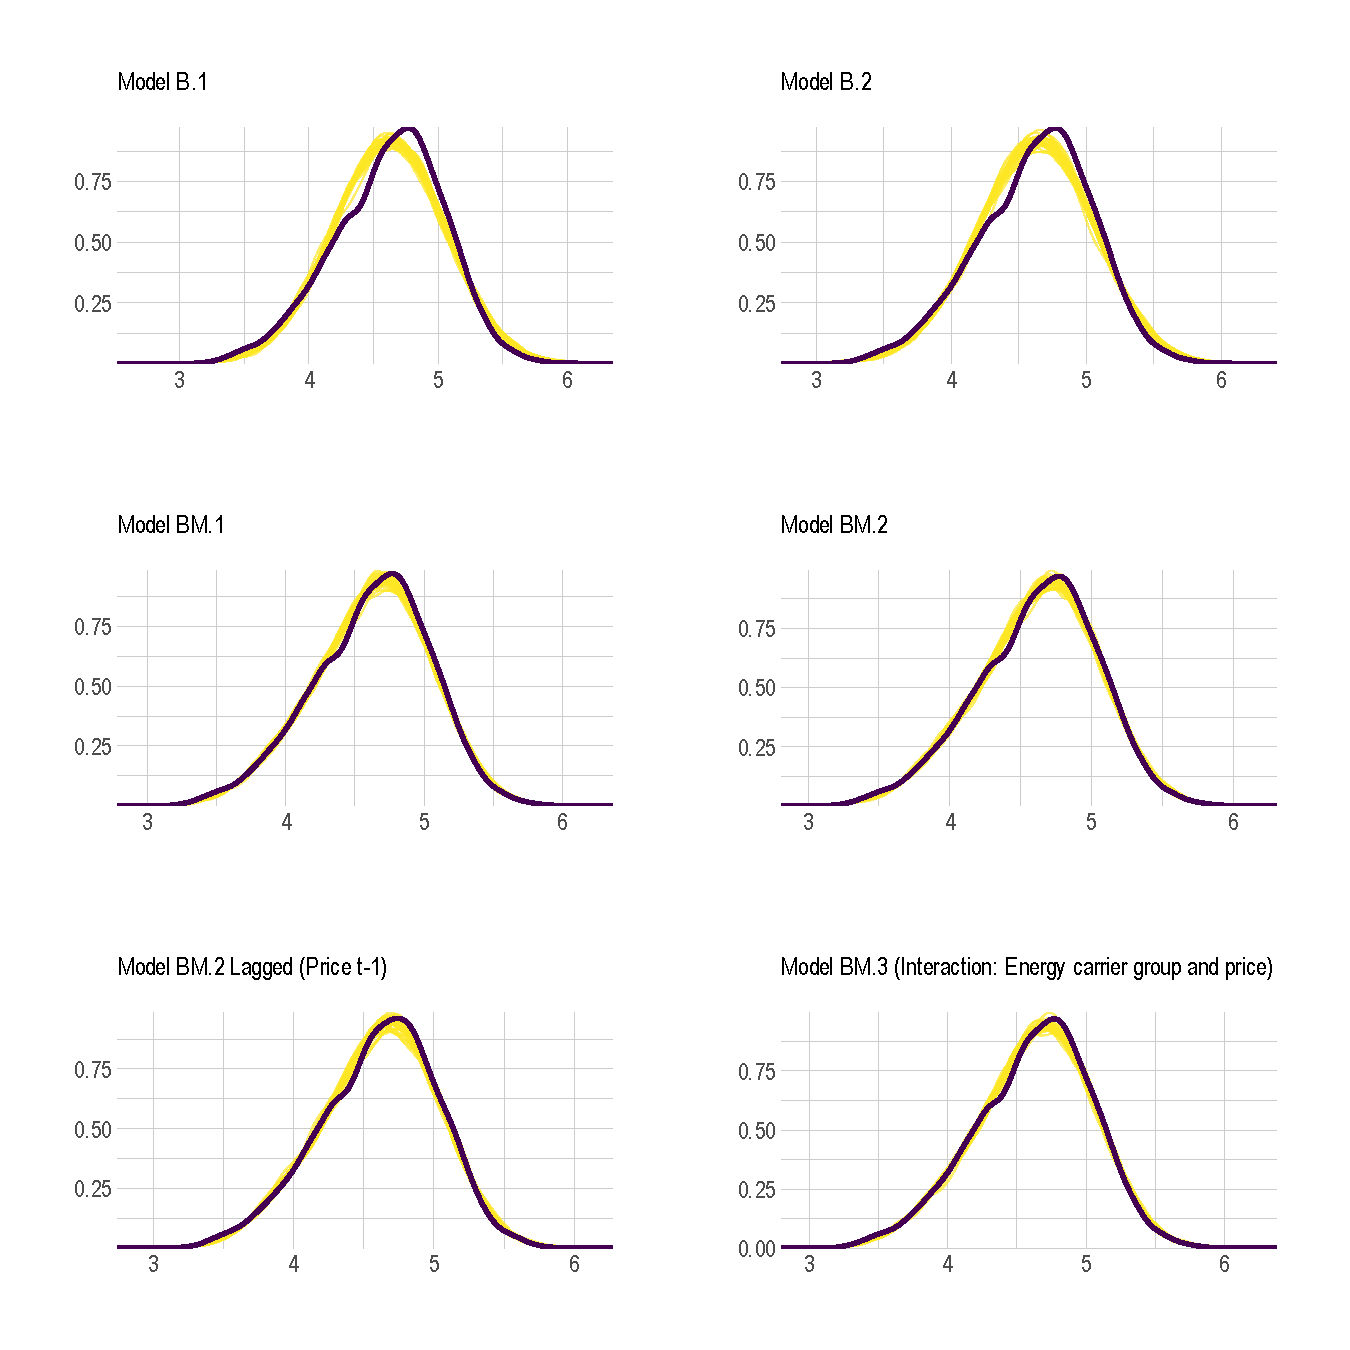
\includegraphics[width=1\linewidth]{figure/plot-model-comparison} 

}

\caption{Graphical model comparison for subsample analysis}\label{fig:plot-model-comparison}
\end{figure}
\noindent
Figure \ref{fig:plot-model-comparison} presents a visual examination of the model fit for all models used on the subsample.

\newpage

\onehalfspacing

\hypertarget{declaration-of-authorship-eigenstuxe4ndigkeitserkluxe4rung}{%
\chapter*{Declaration of Authorship (Eigenständigkeitserklärung)}\label{declaration-of-authorship-eigenstuxe4ndigkeitserkluxe4rung}}
\addcontentsline{toc}{chapter}{Declaration of Authorship (Eigenständigkeitserklärung)}

Hiermit erkläre ich, dass ich die vorliegende Arbeit selbständig verfasst habe und sämtliche Quellen, einschließlich Internetquellen, die unverändert oder abgewandelt wiedergegeben werden, insbesondere Quellen für Texte, Grafiken, Tabellen und Bilder, als solche kenntlich gemacht habe.

Ich versichere, dass ich die vorliegende Abschlussarbeit noch nicht für andere Prüfungen eingereicht habe.

Mir ist bekannt, dass bei Verstößen gegen diese Grundsätze ein Verfahren wegen Täuschungsversuchs bzw. Täuschung gemäß der fachspezifischen Prüfungsordnung und/oder der Fächerübergreifenden Satzung zur Regelung von Zulassung, Studium und Prüfung der Humboldt-Universität zu Berlin (ZSP-HU) eingeleitet wird.

\hfill\break
~

\hfill\break
~

\hfill\break
~
\begin{tabular}{m{6cm}m{2cm}m{6cm}}
Berlin, den 28.02.2022 &  &              \\ \cline{1-1} \cline{3-3} 
\textit{Ort, Datum}            &  & \textit{Unterschrift} \\
                       &  &              \\
                       &  &             
\end{tabular}
\backmatter

\hypertarget{references}{%
\chapter*{References}\label{references}}
\addcontentsline{toc}{chapter}{References}

\markboth{References}{References}

\noindent

\setlength{\parindent}{-0.20in}

\hypertarget{refs}{}
\begin{CSLReferences}{1}{0}
\leavevmode\vadjust pre{\hypertarget{ref-ageb21}{}}%
AGEB. (2021). \emph{Auswertungstabellen zur Energiebilanz 1990 bis 2020}. Berlin. Retrieved from \url{https://ag-energiebilanzen.de/daten-und-fakten/auswertungstabellen/}

\leavevmode\vadjust pre{\hypertarget{ref-alberini_etal11}{}}%
Alberini, A., Gans, W., \& Velez-Lopez, D. (2011). Residential consumption of gas and electricity in the U.S.: The role of prices and income. \emph{Energy Economics}, \emph{33}(5), 870--881. http://doi.org/\href{https://doi.org/10.1016/j.eneco.2011.01.015}{10.1016/j.eneco.2011.01.015}

\leavevmode\vadjust pre{\hypertarget{ref-aldy_etal10}{}}%
Aldy, J. E., Krupnick, A. J., Newell, R. G., Parry, I. W. H., \& Pizer, W. A. (2010). Designing Climate Mitigation Policy. \emph{Journal of Economic Literature}, \emph{48}(4), 903--934. http://doi.org/\href{https://doi.org/10.1257/jel.48.4.903}{10.1257/jel.48.4.903}

\leavevmode\vadjust pre{\hypertarget{ref-auffhammer_rubin18}{}}%
Auffhammer, M., \& Rubin, E. (2018). \emph{Natural Gas Price Elasticities and Optimal Cost Recovery Under Consumer Heterogeneity: Evidence from 300 million natural gas bills} (No. w24295) (p. w24295). Cambridge, MA: National Bureau of Economic Research. Retrieved from \url{http://www.nber.org/papers/w24295.pdf}

\leavevmode\vadjust pre{\hypertarget{ref-bailey17}{}}%
Bailey, M. A. (2017). \emph{Real econometrics: The right tools to answer important questions}. New York: Oxford University Press.

\leavevmode\vadjust pre{\hypertarget{ref-bmwi21}{}}%
BMWi. (2021). \emph{Gesamtausgabe der Energiedaten}. BMWi. Retrieved from \url{https://www.bmwi.de/Redaktion/DE/Binaer/Energiedaten/energiedaten-gesamt-xls.xlsx?__blob=publicationFile\&v=133}

\leavevmode\vadjust pre{\hypertarget{ref-burger_etal19}{}}%
Bürger, V., Hesse, T., Köhler, B., Palzer, A., \& Engelmann, P. (2019). German Energiewende---different visions for a (nearly) climate neutral building sector in 2050. \emph{Energy Efficiency}, \emph{12}(1), 73--87. http://doi.org/\href{https://doi.org/10.1007/s12053-018-9660-6}{10.1007/s12053-018-9660-6}

\leavevmode\vadjust pre{\hypertarget{ref-csereklyei20}{}}%
Csereklyei, Z. (2020). Price and income elasticities of residential and industrial electricity demand in the European Union. \emph{Energy Policy}, \emph{137}, 111079. http://doi.org/\href{https://doi.org/10.1016/j.enpol.2019.111079}{10.1016/j.enpol.2019.111079}

\leavevmode\vadjust pre{\hypertarget{ref-cutler41}{}}%
Cutler, H. A. (1941). The Elasticity of the Residential Demand for Electricity. \emph{The Journal of Land \& Public Utility Economics}, \emph{17}(2), 242--245. http://doi.org/\href{https://doi.org/10.2307/3158428}{10.2307/3158428}

\leavevmode\vadjust pre{\hypertarget{ref-destatis18}{}}%
DESTATIS. (2018). Fernwärmeversorgung 2017: Abgegebene Wärmemenge leicht gesunken. Retrieved January 19, 2022, from \url{https://www.destatis.de/DE/Presse/Pressemitteilungen/2018/11/PD18_434_434.html}

\leavevmode\vadjust pre{\hypertarget{ref-destatis21c}{}}%
DESTATIS. (2021a). Bevölkerung: Kreise, Stichtag, Altersgruppen (12411-0017) {[}Text{]}. Retrieved January 22, 2022, from \url{https://www-genesis.destatis.de/genesis/online?operation=previous\&levelindex=0\&step=0\&titel=Tabellenaufbau\&levelid=1642855066461\&acceptscookies=false\#abreadcrumb}

\leavevmode\vadjust pre{\hypertarget{ref-destatis21}{}}%
DESTATIS. (2021b, November 12). Verbraucherpreisindex: Deutschland, Jahre (61111-0001). Retrieved November 12, 2021, from \url{https://www-genesis.destatis.de/genesis//online?operation=table\&code=61111-0001\&bypass=true\&levelindex=1\&levelid=1636748679996\#abreadcrumb}

\leavevmode\vadjust pre{\hypertarget{ref-erk20}{}}%
ERK. (2020). \emph{Bericht zur Vorjahresschätzung der deutschen Treibhausgasemissionen für das Jahr 2020}. Retrieved from \url{https://expertenrat-klima.de/content/uploads/2021/04/210415_Bericht_Expertenrat_Klimafragen_2021-2.pdf}

\leavevmode\vadjust pre{\hypertarget{ref-europeancomission19}{}}%
European Comission. (2019). \emph{The European Green Deal} (No. COM(2019) 640 final). Brussels. Retrieved from \url{https://eur-lex.europa.eu/legal-content/EN/TXT/HTML/?uri=CELEX:52019DC0640\&from=EN}

\leavevmode\vadjust pre{\hypertarget{ref-gwartney76}{}}%
Gwartney, J. D. (1976). Demand and Consumer Choice. In \emph{Economics Private and Public Choice} (pp. 289--309). Elsevier. http://doi.org/\href{https://doi.org/10.1016/B978-0-12-311050-3.50021-8}{10.1016/B978-0-12-311050-3.50021-8}

\leavevmode\vadjust pre{\hypertarget{ref-halbig_namyslo14}{}}%
Halbig, G., \& Namyslo, J. (2014). Neue Witterungsbereinigung für Energieausweise auf der Basis des Referenzklimas Potsdam. \emph{EneV aktuell}, (4), 11--13.

\leavevmode\vadjust pre{\hypertarget{ref-hennes_etal21}{}}%
Hennes, O., Jeddi, S., Madlener, R., Schmitz, H., Wagner, J., Wolff, S., \& Zinke, J. (2021). Auswirkungen von CO2-Preisen auf den Gebäude‑, Verkehrs- und Energiesektor. \emph{Zeitschrift für Energiewirtschaft}, \emph{45}(2), 91--107. http://doi.org/\href{https://doi.org/10.1007/s12398-021-00305-0}{10.1007/s12398-021-00305-0}

\leavevmode\vadjust pre{\hypertarget{ref-hesse20}{}}%
Heße, W. (2020). \emph{Energieeffiziente Wärmeversorgung von Gebäuden: Tatsächliche Versorgungsverhältnisse und Maßnahmen zur Effizienzsteigerung}. Wiesbaden: Springer Fachmedien Wiesbaden. http://doi.org/\href{https://doi.org/10.1007/978-3-658-27571-6}{10.1007/978-3-658-27571-6}

\leavevmode\vadjust pre{\hypertarget{ref-holland86}{}}%
Holland, P. W. (1986). Statistics and Causal Inference. \emph{Journal of the American Statistical Association}, \emph{81}(396), 945--960. http://doi.org/\href{https://doi.org/10.1080/01621459.1986.10478354}{10.1080/01621459.1986.10478354}

\leavevmode\vadjust pre{\hypertarget{ref-houthakker51}{}}%
Houthakker, H. S. (1951). Some Calculations on Electricity Consumption in Great Britain. \emph{Journal of the Royal Statistical Society. Series A (General)}, \emph{114}(3), 359--371. http://doi.org/\href{https://doi.org/10.2307/2980781}{10.2307/2980781}

\leavevmode\vadjust pre{\hypertarget{ref-iwu21}{}}%
IWU. (2021, October 7). IWU-Tool „Gradtagzahlen-Deutschland.xlsx``. Retrieved January 22, 2022, from \url{https://www.iwu.de/publikationen/fachinformationen/energiebilanzen/}

\leavevmode\vadjust pre{\hypertarget{ref-labandeira_etal17}{}}%
Labandeira, X., Labeaga, J. M., \& López-Otero, X. (2017). A meta-analysis on the price elasticity of energy demand. \emph{Energy Policy}, \emph{102}, 549--568. http://doi.org/\href{https://doi.org/10.1016/j.enpol.2017.01.002}{10.1016/j.enpol.2017.01.002}

\leavevmode\vadjust pre{\hypertarget{ref-lange_etal14}{}}%
Lange, I., Moro, M., \& Traynor, L. (2014). Green hypocrisy?: Environmental attitudes and residential space heating expenditure. \emph{Ecological Economics}, \emph{107}, 76--83. http://doi.org/\href{https://doi.org/10.1016/j.ecolecon.2014.07.021}{10.1016/j.ecolecon.2014.07.021}

\leavevmode\vadjust pre{\hypertarget{ref-leth-petersen_togeby01}{}}%
Leth-Petersen, S., \& Togeby, M. (2001). Demand for space heating in apartment blocks: measuring effects of policy measures aiming at reducing energy consumption. \emph{Energy Economics}, \emph{23}(4), 387--403. http://doi.org/\href{https://doi.org/10.1016/S0140-9883(00)00078-5}{10.1016/S0140-9883(00)00078-5}

\leavevmode\vadjust pre{\hypertarget{ref-levesque_etal21}{}}%
Levesque, A., Pietzcker, R. C., Baumstark, L., \& Luderer, G. (2021). Deep decarbonisation of buildings energy services through demand and supply transformations in a 1.5°C scenario. \emph{Environmental Research Letters}, \emph{16}(5), 054071. http://doi.org/\href{https://doi.org/10.1088/1748-9326/abdf07}{10.1088/1748-9326/abdf07}

\leavevmode\vadjust pre{\hypertarget{ref-loulou_labriet08}{}}%
Loulou, R., \& Labriet, M. (2008). ETSAP-TIAM: the TIMES integrated assessment model Part I: Model structure. \emph{Computational Management Science}, \emph{5}(1-2), 7--40. http://doi.org/\href{https://doi.org/10.1007/s10287-007-0046-z}{10.1007/s10287-007-0046-z}

\leavevmode\vadjust pre{\hypertarget{ref-mcelreath20}{}}%
McElreath, R. (2020). \emph{Statistical Rethinking: A Bayesian Course with Examples in R and Stan} (2nd ed.). Chapman and Hall/CRC. http://doi.org/\href{https://doi.org/10.1201/9780429029608}{10.1201/9780429029608}

\leavevmode\vadjust pre{\hypertarget{ref-meier_rehdanz10}{}}%
Meier, H., \& Rehdanz, K. (2010). Determinants of residential space heating expenditures in Great Britain. \emph{Energy Economics}, \emph{32}(5), 949--959. http://doi.org/\href{https://doi.org/10.1016/j.eneco.2009.11.008}{10.1016/j.eneco.2009.11.008}

\leavevmode\vadjust pre{\hypertarget{ref-metcalf_hassett99}{}}%
Metcalf, G. E., \& Hassett, K. A. (1999). Measuring the Energy Savings from Home Improvement Investments: Evidence from Monthly Billing Data. \emph{Review of Economics and Statistics}, \emph{81}(3), 516--528. http://doi.org/\href{https://doi.org/10.1162/003465399558274}{10.1162/003465399558274}

\leavevmode\vadjust pre{\hypertarget{ref-miller_alberini16}{}}%
Miller, M., \& Alberini, A. (2016). Sensitivity of price elasticity of demand to aggregation, unobserved heterogeneity, price trends, and price endogeneity: Evidence from U.S. Data. \emph{Energy Policy}, \emph{97}, 235--249. http://doi.org/\href{https://doi.org/10.1016/j.enpol.2016.07.031}{10.1016/j.enpol.2016.07.031}

\leavevmode\vadjust pre{\hypertarget{ref-nichols07}{}}%
Nichols, A. (2007). Causal Inference with Observational Data. \emph{The Stata Journal: Promoting Communications on Statistics and Stata}, \emph{7}(4), 507--541. http://doi.org/\href{https://doi.org/10.1177/1536867X0800700403}{10.1177/1536867X0800700403}

\leavevmode\vadjust pre{\hypertarget{ref-osm21a}{}}%
OSM. (2021a). Einwohnerzahl auf PLZ-Gebiete abbilden. Retrieved from \url{https://blog.suche-postleitzahl.org/post/132153774751/einwohnerzahl-auf-plz-gebiete-abbilden}

\leavevmode\vadjust pre{\hypertarget{ref-osm21}{}}%
OSM. (2021b). Postleitzahlen Deutschland. Retrieved from \url{https://www.suche-postleitzahl.org/downloads}

\leavevmode\vadjust pre{\hypertarget{ref-pindyck_rubinfeld18}{}}%
Pindyck, R. S., \& Rubinfeld, D. L. (2018). \emph{Microeconomics} (9th Edition). New York, NY: Pearson.

\leavevmode\vadjust pre{\hypertarget{ref-rehdanz07}{}}%
Rehdanz, K. (2007). Determinants of residential space heating expenditures in Germany. \emph{Energy Economics}, \emph{29}(2), 167--182. http://doi.org/\href{https://doi.org/10.1016/j.eneco.2006.04.002}{10.1016/j.eneco.2006.04.002}

\leavevmode\vadjust pre{\hypertarget{ref-rwi21}{}}%
RWI. (2021). \emph{Anwendungsbilanzen 2020 für den Sektor der privaten Haushalte und den Verkehrssektor in Deutschland}. Retrieved from \url{https://ag-energiebilanzen.de/wp-content/uploads/2020/10/rwi_anwendungsbilanz_2020__priv._hh_und_verkehr__vorl._eb.pdf}

\leavevmode\vadjust pre{\hypertarget{ref-schmitz_madlener20}{}}%
Schmitz, H., \& Madlener, R. (2020). Heterogeneity in price responsiveness for residential space heating in Germany. \emph{Empirical Economics}, \emph{59}(5), 2255--2281. http://doi.org/\href{https://doi.org/10.1007/s00181-019-01760-y}{10.1007/s00181-019-01760-y}

\leavevmode\vadjust pre{\hypertarget{ref-schulte_heindl17}{}}%
Schulte, I., \& Heindl, P. (2017). Price and income elasticities of residential energy demand in Germany. \emph{Energy Policy}, \emph{102}, 512--528. http://doi.org/\href{https://doi.org/10.1016/j.enpol.2016.12.055}{10.1016/j.enpol.2016.12.055}

\leavevmode\vadjust pre{\hypertarget{ref-statistischeamter21}{}}%
Statistische Ämter. (2021). Einkommen der privaten Haushalte in den kreisfreien Städten und Landkreisen der Bundesrepublik Deutschland 1995 bis 2019. Retrieved November 12, 2021, from \url{http://www.statistikportal.de/de/vgrdl/ergebnisse-kreisebene/einkommen-kreise}

\leavevmode\vadjust pre{\hypertarget{ref-stede_etal20}{}}%
Stede, J., Schütze, F., \& Wietschel, J. (2020). Wärmemonitor 2019: Klimaziele bei Wohngebäuden trotz sinkender CO2-Emissionen derzeit außer Reichweite (Version 2.0). \emph{DIW Wochenbericht}. http://doi.org/\href{https://doi.org/10.18723/DIW_WB:2020-40-1}{10.18723/DIW\_WB:2020-40-1}

\leavevmode\vadjust pre{\hypertarget{ref-stiglitz19}{}}%
Stiglitz, J. (2019). \emph{Addressing Climate Change through Price and Non-Price Interventions} (No. w25939) (p. w25939). Cambridge, MA: National Bureau of Economic Research. Retrieved from \url{http://www.nber.org/papers/w25939.pdf}

\leavevmode\vadjust pre{\hypertarget{ref-techem19}{}}%
Techem. (2019). \emph{Energiekennwerte 2019}. Eschborn: Techem. Retrieved from \url{https://www.techem.com/content/dam/techem/newsroom/studien/Techem-Energiekennwerte-Studie-2019.pdf}

\leavevmode\vadjust pre{\hypertarget{ref-uba16}{}}%
UBA. (2016). \emph{CO2-Emissionsfaktoren für fossile Brennstoffe}. Retrieved from \url{https://www.umweltbundesamt.de/sites/default/files/medien/1968/publikationen/co2-emissionsfaktoren_fur_fossile_brennstoffe_korrektur.pdf}

\leavevmode\vadjust pre{\hypertarget{ref-varian10}{}}%
Varian, H. R. (2010). \emph{Intermediate microeconomics: a modern approach} (8th Edition). New York, NY: Norton.

\leavevmode\vadjust pre{\hypertarget{ref-vdi13}{}}%
VDI. (2013). \emph{Richtlinie 3807 Blatt 1: Verbrauchskennwerte für Gebäude}. Retrieved from \url{https://www.vdi.de/richtlinien/details/vdi-3807-blatt-1-verbrauchskennwerte-fuer-gebaeude-grundlagen-1}

\leavevmode\vadjust pre{\hypertarget{ref-wooldridge13}{}}%
Wooldridge, J. M. (2013). \emph{Introductory econometrics: a modern approach} (5th edn). Mason: South-Western Cengage Learning.

\end{CSLReferences}

% Index?

\end{document}
